\documentclass[magyar,]{book}
\usepackage{lmodern}
\usepackage{amssymb,amsmath}
\usepackage{ifxetex,ifluatex}
\usepackage{fixltx2e} % provides \textsubscript
\ifnum 0\ifxetex 1\fi\ifluatex 1\fi=0 % if pdftex
  \usepackage[T1]{fontenc}
  \usepackage[utf8]{inputenc}
\else % if luatex or xelatex
  \ifxetex
    %\usepackage{mathspec}
	\usepackage{fontspec}
	\usepackage{unicode-math}
  \else
    \usepackage{fontspec}
	\usepackage{unicode-math}
  \fi
  \defaultfontfeatures{Ligatures=TeX,Scale=MatchLowercase}
    \setmainfont[]{XITS}
    \setmathfont[]{XITS Math}
\fi
% use upquote if available, for straight quotes in verbatim environments
\IfFileExists{upquote.sty}{\usepackage{upquote}}{}
% use microtype if available
\IfFileExists{microtype.sty}{%
\usepackage{microtype}
\UseMicrotypeSet[protrusion]{basicmath} % disable protrusion for tt fonts
}{}
\usepackage{hyperref}
\hypersetup{unicode=true,
            pdftitle={A valószínűségszámítás és a statisztika alapvonalai},
            pdfauthor={Ferenci Tamás},
            pdfborder={0 0 0},
            breaklinks=true}
\urlstyle{same}  % don't use monospace font for urls
%\ifnum 0\ifxetex 1\fi\ifluatex 1\fi=0 % if pdftex
  \usepackage[shorthands=off,main=magyar]{babel}
%\else
%  \usepackage{polyglossia}
%  \setmainlanguage[]{magyar}
%%\fi
\usepackage{longtable,booktabs}
\usepackage{graphicx,grffile}
\makeatletter
\def\maxwidth{\ifdim\Gin@nat@width>\linewidth\linewidth\else\Gin@nat@width\fi}
\def\maxheight{\ifdim\Gin@nat@height>\textheight\textheight\else\Gin@nat@height\fi}
\makeatother
% Scale images if necessary, so that they will not overflow the page
% margins by default, and it is still possible to overwrite the defaults
% using explicit options in \includegraphics[width, height, ...]{}
\setkeys{Gin}{width=\maxwidth,height=\maxheight,keepaspectratio}
\IfFileExists{parskip.sty}{%
\usepackage{parskip}
}{% else
\setlength{\parindent}{0pt}
\setlength{\parskip}{6pt plus 2pt minus 1pt}
}
\setlength{\emergencystretch}{3em}  % prevent overfull lines
\providecommand{\tightlist}{%
  \setlength{\itemsep}{0pt}\setlength{\parskip}{0pt}}
\setcounter{secnumdepth}{5}
% Redefines (sub)paragraphs to behave more like sections
\ifx\paragraph\undefined\else
\let\oldparagraph\paragraph
\renewcommand{\paragraph}[1]{\oldparagraph{#1}\mbox{}}
\fi
\ifx\subparagraph\undefined\else
\let\oldsubparagraph\subparagraph
\renewcommand{\subparagraph}[1]{\oldsubparagraph{#1}\mbox{}}
\fi

%%% Use protect on footnotes to avoid problems with footnotes in titles
\let\rmarkdownfootnote\footnote%
\def\footnote{\protect\rmarkdownfootnote}

%%% Change title format to be more compact
\usepackage{titling}

% Create subtitle command for use in maketitle
\providecommand{\subtitle}[1]{
  \posttitle{
    \begin{center}\large#1\end{center}
    }
}

\setlength{\droptitle}{-2em}

  \title{A valószínűségszámítás és a statisztika alapvonalai}
    \pretitle{\vspace{\droptitle}\centering\huge}
  \posttitle{\par}
    \author{Ferenci Tamás}
    \preauthor{\centering\large\emph}
  \postauthor{\par}
      \predate{\centering\large\emph}
  \postdate{\par}
    \date{2019. november 9.}

\usepackage{booktabs}
\usepackage{csquotes}
\usepackage{epigraph}
\renewcommand{\textflush}{flushright}
\usepackage{tikz}

\begin{document}
\maketitle

{
\setcounter{tocdepth}{1}
\tableofcontents
}
\hypertarget{elux151szuxf3}{%
\chapter*{Előszó}\label{elux151szuxf3}}
\addcontentsline{toc}{chapter}{Előszó}

\epigraph{Ez a visszavezetés a lényege a [...] megoldásnak, nem a képlet.}{\textit{Péter Rózsa}}

Ez a jegyzet egy kísérlet. Kísérlet arra, hogy a valószínűségszámítás és a statisztika alapjait elmagyarázza, de a nélkül, hogy ehhez matematikai formalizmust használna. Nem lesznek benne tételek, levezetések, bizonyítások, sőt, még a szimbolikus jelölések bevezetését is igyekeztem a lehető legszükségesebbre korlátozni.

Mi motiválja ezt a kísérletet? A valószínűségszámítás és a statisztika szokásos egyetemi tárgyalása matematikailag formalizált. Hol mélyebb apparátust használ, hol világosabbat, de mindenesetre végig matematizált. Ami, félreértés ne essék, teljesen érthető, hiszen mind a valószínűségszámításnak, mind a statisztikának a korszerű felépítése csakugyan jól formalizált, és ez elengedhetetlenül szükséges is a bonyolultabb koncepciók bevezetésével és tárgyalásához.

A tapasztalatom azonban az, hogy rengeteg olyan hallgató van, orvostanhallgatók, szociológusok, biológusok, akik abba a furcsa helyzetbe kerülnek, hogy egyfelől a matematikai formalizmusra sem szükségük nincsen, sem kézbentartani nem tudják, de másfelől borzasztó fontos lenne, hogy az alapgondolatokat jól megértsék. Úgy érzem, hogy a matematizált tárgyalás az esetükben egy rossz kompromisszumot köt: azért, hogy a bonyolultabb dolgok is elmondhatóak legyenek (mert ahhoz tényleg kell a matematikai formalizmus, nem kérdés!), az egyszerűbbeket is úgy mondja el, hogy nem értik meg azok, akiknek a bonyolultabbakra nincs szükségük. De miért ne mondjuk inkább ez az egyszerűbbeket formalizáltság nélkül? Igen, így a bonyolultabbakat nem lehet elmondani, de ha egyszer ezekre úgysem lesz szükségük (illetve az érdeklődők úgyis el tudják sajátítani)\ldots? Nem lenne jobb kompromisszum feláldozni a bonyolultabb dolgokat cserében azért, hogy az egyszerűek jobban érthetőek legyenek? Hiszek ugyanis abban, hogy a valószínűségszámítás és a statisztika alapjait -- amik sok szakmában az igazán fontosak! -- igenis el lehet mondani matematikai formalizmus nélkül is érthetően, világosan.

A cél elérése érdekében igyekszem sokkal nagyobb figyelmet szentelni annak, hogy az alapgondolatok jól követhetőek legyenek, több oldalról körüljárni őket, megmutatni az alkalmazásaikat, példát hozni, ahol lehet szimulációkat végezni, sőt, a jegyzet webes változatában interaktív vizualizációkat is mutatni.

Az olvasó a kísérlet eredményét a jegyzet végére megítélheti. Én mindenesetre -- különösen azért, mert ez egy kísérlet -- minden visszajelzést, véleményt, kritikát a lehető legnagyobb örömmel veszek a \url{tamas.ferenci@medstat.hu} email-címen!

\hypertarget{a-valuxf3szuxednux171suxe9gszuxe1muxedtuxe1s-ruxf6viden}{%
\chapter{A valószínűségszámítás röviden}\label{a-valuxf3szuxednux171suxe9gszuxe1muxedtuxe1s-ruxf6viden}}

\epigraph{A valószínűségszámítás nem más, mint számokra átváltott józan ész.}{\textit{Pierre-Simon de Laplace}}

A statisztikusok számára a valószínűség-számítás vagy -- rosszabb esetben -- gonosz nagytestvér, akire titokban irigykedik mindenki, mert az \enquote{igazi} matematika, cserében a felét nem érti az ember, vagy -- jobb esetben -- az a segédtudomány, de jobb lenne azt mondani: alaptudomány, amihez egy halom esetben vissza lehet nyúlni a statisztikai problémák kezelése során. A valószínűségszámítás megértése tehát megkerülhetetlen (pontosabban szólva: nem érdemes megkerülni!) ahhoz, hogy az ember jól megértse a statiszikát. Nem kell valószínűségszámítási szaktudósnak lenni, ellenkezőleg, pár alapfogalom lesz csak igazán fontos -- de azokat tényleg jól kell érteni.

Ez a fejezet ezt a célt szolgálja. Összhangban az Előszóval mondottakal, kerülni fogok minden matematikai formalizmust, képletet, levezetést, szépen kimondott tételt, ami tudom, hogy elkerülhetetlenül trehányságokhoz fog vezetni, ezért előre valszámos barátaink elnézését kérem, de cserében igyekszem hangsúlyozni azokat a koncepciókat, amiket fontos átlátni a későbbiekhez. (A statisztika és a valószínűségszámítás viszonyára pedig még visszatérek később, amikor mindkettő megfelelő fogalmai és problémái ismertek lesznek.)

\hypertarget{mi-az-hogy-vuxe9letlen}{%
\section{Mi az, hogy véletlen?}\label{mi-az-hogy-vuxe9letlen}}

\epigraph{Mert töredékes az ismeretünk, és töredékes a prófétálásunk.}{\textit{Szent Pál}}

Szokták mondani, hogy a valószínűségszámítás alapfogalma a \textbf{véletlen kísérlet} és hogy ennek definíciója: valami, ami adott körülmények között akárhányszor végrehajtható vagy megfigyelhető, de a kimenete nem mondható meg biztosan (csak az ismert, hogy milyen kimenetei lehetségesek egyáltalán), például mert az ismereteink hiányosak, hogy pontosan meg tudjuk előre mondani a kimenetet.

Az elnevezés második szava jó szerencsétlen, mert a valószínűségszámítás egy halom olyan dolgot vizsgál, ami nem kísérlet a szó szokásos tudományos értelmében, azaz nem mi hajtjuk végre, de még csak az sem világos első látásra, hogy milyen értelemben ismételhető meg akárhányszor. Az orvostudományban vizsgálhatjuk például azt, hogy egy beteg meggyógyul-e. Hogy ez nagyon sokszor tényleg olyan, ami nem mondható meg biztosan, az vitathatatlan, na de hogy kísérlet? És akárhányszor megfigyelhető?! A pszichológiából, szociológiából stb. nem csak hogy milliónyi hasonló példát lehetne hozni, de ezeken a területeken pont hogy \emph{nem} tipikus, hogy kísérletet végzünk. Fogjuk fel ezt hagyományos elnevezésként, ami az olyan hétköznapi példákból jött mint a kockadobás, amit tényleg napestig ismételgethetünk azonos körülmények között, kísérletként.

A \enquote{véletlen} szó viszont látszólag teljesen rendben van, ez tényleg jól megfelel nyelvileg annak, hogy \enquote{a kimenete nem mondható meg biztosan}. Valójában ezen is érdemes kicsit elmorfondírozni. A Mi a véletlen? kérdés nagy részét átutalom a filozófia tárgykörébe, itt most egy aspektust szeretnék érinteni: azt, hogy a válasz nagyon gyakran igazából azon is múlik, hogy mi milyen közelítési pontosságot választunk, mit hanyagolunk el és mit nem. Vegyük a kockadobást! Az előző bekezdésben is szerepelt, mint valami \enquote{nyilvánvalóan} jó példa a véletlenre, de ha jobban meggondoljuk, akkor \emph{igazából} a kockadobás kimenete -- az előbbi értelemben -- \emph{nem} véletlen, mert nagyon is megmondható: ha ismerjük az eldobás pillanatában a kocka sebességét, gyorsulását, a légellenálással kapcsolatos adatait, az ütközési tényezőjét az asztallal találozáskor stb. akkor \emph{elvileg} tökéletesen pontosan, \emph{determinisztikusan} megmondható, hogy hányast fog mutatni, ehhez csak a fizikát kell tudni. Ha valaki azt gondolná, hogy ez csak ilyen elvi jelentőségű, akadémikus akadékoskodás, akkor gondoljon arra, hogy pár évvel ezelőtt a laikus sajtóban is hír volt az az okostelefonra fejlesztett alkalmazás, amivel ha az ember levideóz egy rulettkereket, akkor még pörgés \emph{közben} meg tudja jó eséllyel mondani, hogy hová fog érkezni a golyó! (Ezen képesség szerény kezdőtőke birtokában nagyon is gyakorlati jelentőségű és kevéssé akadémikus előnyökre átváltható.) Pedig hát a rulettkerék pörgetésénél ideáltipikusabb példát aligha lehet találni arra, hogy mi \enquote{véletlen}\ldots{} És tessék -- ugyanazon múlt a dolog, hogy a kameraképen megkeressük a golyót, meghatározzuk a gyorsulását, ezt bedobjuk a mozgására vonatkozó fizikai egyenletekbe stb., és így egy sztochasztikus dolgot determinisztikussá teszünk.

Úgyhogy fogalmazzunk úgy: a továbbiakban olyan jelenségekkel foglalkozunk, amik az \emph{aktuális közelítési szintünkön} véletlenek. Persze jobb, ha ezek véletlenségét ki tudjuk küszöbölni, de akkor is kell valamit tennünk, ha erre nincs mód (mint ahogy sok esetben nincs, és a belátható jövőben nem is lesz). Ekkor fog jól jönni a valószínűségszámítás.

\hypertarget{a-valuxf3szuxednux171suxe9gszuxe1muxedtuxe1s-alapfogalmai}{%
\section{A valószínűségszámítás alapfogalmai}\label{a-valuxf3szuxednux171suxe9gszuxe1muxedtuxe1s-alapfogalmai}}

Most hogy tisztáztuk a véletlen kísérlet tartalmát, menjünk tovább az alapfogalmak bevezetésében. Mindenekelőtt szükségünk van a véletlen kísérlet lehetséges kimeneteleire, ezeket, roppant kreatív módon, hivatalosan \textbf{kimenetelnek} nevezzük\footnote{Némelyik magyar irodalom a kimenetel helyett az elemi esemény terminológiát használja. Ez azonban nem egységes, az angol irodalom egységesen \emph{nem} ezt hívja elemi eseménynek, ráadásul a kimenetel szó némileg logikusabb is, úgyhogy a továbbiakban ezt fogom használni.}, kockadobásnál ilyen a ⚀ vagy a ⚂ (szándékosan nem számot írtam!). A kimenetelekből mindig \emph{pontosan} egy következik be: nem lehet az, hogy kettő (nem dobhatok egyszerre ⚀-et és ⚂-at), és nem lehet az sem, hogy egy sem (nem lehet, hogy amit dobok az nem ⚀, nem ⚁, nem ⚂, nem ⚃, nem ⚄ és nem ⚅). A lehetséges kimenetelek összességét, tehát mindent ami kijöhet a kísérletből, \textbf{eseménytérnek} szokás nevezni. Valamilyen dolgokat akarok összefogni\ldots{} erre a jó matematikai objektum a halmaz lesz! Tehát az eseménytér egy halmaz, ami minden lehetséges kimenetelt tartalmaz. A kockadobásnál: \(\left\{⚀,⚁,⚂,⚃,⚄,⚅\right\}\).

Ez egy meglehetősen egyszerű helyzet, hiszen az eseménytér véges sok kimenetelből áll. Bonyolultabb a szituáció akkor, ha mondjuk azt vizsgáljuk, hogy egy véletlenszerűen kiválasztott magyar lakos hányszor járt külföldön életében. Ez lehet 0, 1, 2, 3, 4,\ldots{} de hol a vége? A válasz az, hogy \emph{sehol}! Semmilyen számra nem mondhatjuk azt, hogy na, legfeljebb ennyiszer lehetett külföldön járni\ldots! (Az rossz érvelés, hogy nézzük meg, hogy mennyi az eddigi magyar rekorder. Mondjuk azt találjuk, hogy 123-szor járt külföldön\ldots{} és? Akkor mondhatjuk, hogy legfeljebb 123-szor lehet külföldön járni? Nyilván nem, a világon semmi akadálya nincs, hogy valaki 124-szer járjon. De akkor 124 a maximum? Nem, miért ne lehetne utána még egyet utazni.) Összességében tehát világos, hogy az \emph{nem korlátos}, hogy valaki hányszor járhatott külföldön, így az eseménytér a \(\left\{\text{,,0-szor járt''},\text{,,1-szer járt''}, \text{,,2-szer járt''},\dots{}\right\}\) halmaz. Ez tehát már végtelen halmaz! De a matematikusok úgy mondják: megszámlálhatóan végtelen, ami azt jelenti, hogy végtelen ugyan, de az elemeit fel lehet sorolni egymás után (hát persze, az előbb ezt meg is tettük). Még durvább a helyzet akkor, ha mondjuk azt kérdezzük, hogy mekkora egy véletlenszerűen kiválasztott ember testtömege. Lehet mondjuk 70 kg, de lehet 70,5 is. Vagy 70,48. Vagy 70,477. Vagy 70,4779. Azaz ez is végtelen sok értéket vehet fel! (Valaki azt mondhatja, hogy de hát a mérlegen csak az egész kilogrammokat lehet leolvasni. Persze, így tényleg véges sok érték lehetséges csak, de vegyünk jobb mérleget, amin tizedek is vannak. Még jobbat, amin századok is, és így tovább. A lényeg, hogy \emph{elvileg} a testtömeg bármilyen valós szám lehet, most függetlenítsük magunkat attól, hogy a mérőeszközünk ezt csak korlátozott pontossággal tudja lemérni, vegyük úgy, hogy a vizsgált jellemző az \emph{igazi} testtömeg, mintha lenne korlátlan pontosságú mérlegünk.) Ez tehát végtelen sok lehetséges kimenet, de az előzőnél is jobban végtelen, abban az értelemben, hogy ezeknek az elemeit már fel sem lehet sorolni! (Azaz nem lehet megmondani, hogy egy adott értékre mi a rákövetkező. Mert egész számok körében világos, hogy 70 után 71 jön. De a valós számok között mi jön a 70 után? 70,1? Nem, mert a 70,01 közelebb van. Akkor 70,01? Nem, mert a 70,001 közelebb van. Akkor 70,001? És így tovább, szóval a valós számok \enquote{jobban végtelenen} vannak mint az egészek, hiszen fel sem lehet őket sorolni; ezt szokták nem megszámlálható végtelennek nevezni.) Az érdekes az, hogy az ember azt gondolná, hogy a három eset között a nagy különbség ott van, hogy az eseménytér véges vagy végtelen, az már részletkérdés, hogy mennyire -- megszámlálhatóan vagy nem megszámlálhatóan -- végtelen. Ez nem így van! A helyzet az, hogy a véges és a megszámlálhatóan végtelen eset kezelése nagyon hasonló, ami igazán eltér, az a megszámlálhatatlanul végtelen eseménytér. A véges, vagy legfeljebb megszámlálhatóan végtelen eseményteret \textbf{diszkrét} eseménytérnek, a nem megszámlálhatóan végtelen eseményteret \textbf{folytonos} eseménytérnek szokták nevezni.

Most, hogy ezeken túl vagyunk, jöhetnek végre a valószínűségek! Ha már kimeneteleink vannak, akkor azt gondolhatnánk, hogy azokhoz szeretnénk valószínűséget rendelni, például megmondani, hogy mekkora valószínűséggel dobunk ⚀-et. Nem ezt fogjuk tenni! Szeretnénk ugyanis valószínűséget rendelni bonyolultabb dolgokhoz is, például ahhoz, hogy \enquote{páros számot dobunk}. Ennek megragadásához ismét a halmazokhoz fordulunk: a kimenetelekből egyet vagy többet bepakolunk egy halmazba, mondjuk így: \(\left\{⚁,⚃,⚅\right\}\) ,elnevezzük ezt \textbf{eseménynek} és azt mondjuk, hogy egy esemény akkor következik be, ha olyan kimenetel áll elő, ami az eseménynek -- mint halmaznak -- az eleme. Világos tehát, hogy az előbbi esemény tényleg azt jelenti, hogy \enquote{páros számot dobtunk}. Hasonlóképp definiálhatunk tetszőleges további eseményt. Például a \(\left\{⚀,⚁,⚂,⚃\right\}\) esemény akkor következik be, ha ⚀-et dobunk, ⚁-t dobunk, ⚂-t dobunk vagy ⚃-et dobunk, hiszen egy esemény akkor következik be, ha olyan kimenetel jön ki, ami benne, mint halmazban benne van -- magyarul elmondva ez lesz az, hogy \enquote{4-nél nem nagyobb számot dobtunk}. Az eseményeket általában az \(A\), \(B\), \(C\), \ldots{} betűkkel jelöljük, például \(A=\left\{⚁,⚃,⚅\right\}\).(De akkor azt nem is tudjuk megmondani, hogy mekkora valószínűséggel dobunk ⚀-et?! Dehogynem! Vegyük azt az -- \emph{egyelemű!} -- halmazt, hogy \(\left\{⚀\right\}\), és meg is vagyunk! A világon semmi nem tiltja, hogy egy eseménybe csak egyetlen kimenetelt pakoljunk be. Világos tehát, hogy ez a megközelítés csak általánosítja, kiterjeszti azt, mintha a kimentelekhez rendelnénk valószínűségeket.) Természetesen az is egy esemény, ami az összes kimenetelt tartalmazza (vagyis az esemény maga az eseménytér), ezt szokták biztos eseménynek nevezni, és az üres halmaz is egy esemény, ezt pedig lehetetlen eseménynek hívjuk. Az elnevezések teljesen logikusak: a biztos esemény biztosan bekövetkezik, hiszen mindenképp olyan kimenetel jön ki, ami benne van (lévén, hogy az összes benne van), a lehetetlen pedig soha, hiszen egyetlen kimenetel sincsen benne (mivel üres halmaz), azaz bármelyik kimenetel is következik be, soha nem lesz igaz, hogy a bekövetkező kimenetel benne van.

Ennek a megközelítésnek van még egy előnye. Mondjuk, hogy szeretnénk arról az eseményről beszélni, hogy \enquote{4-nél nem nagyobb páros számot dobunk}. Mi lesz ennek a halmaza? \(\left\{⚁,⚃\right\}\). De vegyük észre, hogy ez nem más, mint a két előző halmaz metszete! Persze, mert annak, hogy \enquote{4-nél nem nagyobb \emph{és} páros} azok a kimenetelek felelnek meg (azok kijövetele esetén következik be ez az esemény), amik \emph{egyszerre} benne vannak abban, hogy \enquote{4-nél nem nagyobb} \emph{és} abban, hogy \enquote{páros}. Az események \enquote{és}-sel történő összekapcsolásának tehát megfelel az, hogy a halmazaik metszetét képezzük. Kitérő megjegyzés: ha két esemény metszete üres halmaz, az magyarul azt jelenti, hogy nem következhetnek be egyszerre (például \enquote{2-nél nem nagyobbat dobunk} és \enquote{4-nél nem kisebbet dobunk}); ezeket szokás kizáró eseménynek nevezni. Továbbmenve, annak az eseménynek, hogy \enquote{4-nél nem nagyobb vagy páros számot dobunk} a két halmaz uniója fog megfelelni, gondoljuk végig. Tehát a \enquote{vagy}-gyal történő összekapcsolásnál sem kell semmin gondolkoznunk, a \enquote{vagy} használatával kapott esemény(nek megfelelő halmaz) a két esemény, mint halmaz uniója lesz. Egy szó mint száz, azt látjuk, hogy az események ilyen \enquote{verbális} képzésének megfeleltethetünk szokásos halmazelméleti műveleteket.

A végére még egy, de fontos megjegyzés. Valaki ezen a ponton esetleg azt mondhatja, hogy ne is gondolkozzunk azon, hogy mely eseményekhez rendelünk valószínűséget, egyszerűen vegyük a kimenetelekből képezett \emph{összes lehetséges} halmazt (az üres halmazt, az összes kimenetelt mint egyelemű halmazt, az összes két kimenetelből álló eseményt, és így tovább, egészen az összes öt kimenetelből álló halmazig, és végül az egész eseménytérig). És akkor nem kell semmin gondolkoznunk, bárkinek bármilyen esemény jut is az eszébe, mindegyikhez lesz valószínűség. Ez nagyon csábítóan hangzik -- de sajnos nem fog működni. Hogy egész pontos legyek, diszkrét eseménytereknél működik, ott nyugodtan csinálhatjuk ezt, de folytonos esetekben nagyon csúnya dolgok történnének, ha megpróbálnánk szó szerint minden elképzelhető eseményhez valószínűséget rendelni. Éppen ezért be kell vezetnünk még egy fogalmat: azon események halmazát, amihez szeretnénk egyáltalán valószínűséget rendelni. Diszkrét esetben ez lehet az összes lehetséges esemény, de folytonos esetben szűkebb lesz nála. A dolgot nem tehetjük meg akárhogy, bizonyos követelményeket ki kell elégítenünk (csak példának okáért: ha két eseményhez rendelünk valószínűséget, akkor kötelező az uniójukhoz, tehát a \enquote{vagy}-gyal összekapcsoltjukhoz is rendelni valószínűséget, de igaz lesz az is, hogy az \enquote{és}-sel összekapcsoltjukhoz is kell legyen valószínűség rendelve), de ez most számunkra nem annyira fontos, a lényeg, hogy lesz egy halmazunk, amikben azok az események vannak, amikhez valószínűséget rendelünk. Hívjuk ezt a \textbf{megfigyelhető események} halmazának. (Ez inkább csak terminológia, ne akarjunk szükségképp a \enquote{megfigyelés} hétköznapi szavával kapcsolatba hozni. Fogjuk fel úgy, hogy ez egy elnevezés, egyszerűen így hívjuk azokat az eseményeket, amikhez valószínűséget fogunk rendelni.)

\hypertarget{a-valuxf3szuxednux171suxe9g-bevezetuxe9se}{%
\section{A valószínűség bevezetése}\label{a-valuxf3szuxednux171suxe9g-bevezetuxe9se}}

És akkor végre: jöhet a valószínűség! A fentiek után a dologban nem lesz sok meglepetés: a \textbf{valószínűség} egy függvény, amely a megfigyelhető események mindegyikéhez hozzárendel egy valós számot. Például lehet egy ilyen hozzárendelés egyik eleme az, hogy \(\left\{⚁,⚃,⚅\right\}\mapsto0,\!3\). Azaz a \enquote{párosat dobunk} eseményhez 0,3 valószínűséget rendelünk. (Hétköznapi szóhasználatban azt mondanánk: 30\%. A kettő ugyanaz, hiszen a százalékjel egyszerűen egy \enquote{szorozva 0,01-gyel}-t helyettesít. A valószínűségszámításban, matematikában egyszerűbb az élet, ha 0,3-at mondunk.) A valószínűség jele\footnote{A könyvek egy része \(\mathbf{P}\)-t használ, tehát vastagon szedi a betűt. Kézírásban persze senki nem fog nekiállni satírozgatni minden betűnél, ezért gyakran \enquote{duplaszárú} betűt használnak, ami viszont nagyon menőn néz ki, ezért érdekes módon visszaszivárgott a gépi szedésbe; én is ezt fogom használni.} \(\mathbb{P}\), tehát \(A\) esemény valószínűséget \(\mathbb{P}\left(A\right)\)-val jelöljük, előbbi példánkban: \(\mathbb{P}\left(A\right)=\mathbb{P}\left(\left\{⚁,⚃,⚅\right\}\right)=0,\!3\).

És meg is vagyunk, ez a valószínűség!

Ez eddig igazán nem agysebészet, de az érdekes rész most jön. 1933-ban Kolmogorov szovjet matematikus azt mondta, hogy három dolgot \emph{követeljünk meg} ettől a függvénytől. Tehát ne \emph{akárhogy} rendeljünk valószínűségeket a megfigyelhető eseményekhez, hanem csak az lesz elfogadható hozzárendelés, ami a következő három dolgot tudja:

\begin{enumerate}
\def\labelenumi{\arabic{enumi}.}
\tightlist
\item
  A valószínűségek nemnegatívak (nem lehet olyan, hogy például \(\left\{⚁,⚃,⚅\right\}\mapsto- 0,\!2\)).
\item
  A biztos esemény valószínűsége 1 (nem lehet olyan, hogy például \(\left\{⚀,⚁,⚂,⚃,⚄,⚅\right\}\mapsto 1,\!1\) vagy \(\left\{⚀,⚁,⚂,⚃, ⚄ ,⚅ \right\}\mapsto 0,\!7\)).
\item
  Kizáró események uniójának, tehát \enquote{vagy}-gyal összekapcsoltjának a valószínűsége a valószínűségeik összege (nem lehet olyan, hogy például \(\left\{⚀,⚁\right\}\mapsto 0,\!1\) és \(\left\{⚄,⚅\right\}\mapsto 0,\!2\), de közben \(\left\{⚀,⚁,⚄,⚅\right\}\mapsto 0,\!4\)).
\end{enumerate}

Magyarázatot igazából csak a legutolsó követelmény érdemel, a másik kettő megfelel annak, amit a \enquote{valószínűség} fogalomról hétköznapilag is mondanánk. A harmadik követelmény megértéséhez a legjobb, ha úgy gondolunk az eseményekre mint pacákra egy festővásznon. Még jobb, ha úgy vesszük, hogy a kimenetelek pontok, és az események, a pacák, úgy készültek, hogy egy vagy több pontot lefestettünk adott színnel. Egy jó elképzelés, és nem csak a szemléletesség kedvéért, hanem mélyebb értelemben is, ha a valószínűségre úgy gondolunk, mint a pacák \emph{területére}. (Ez az első két axiómát is szépen hozza: az első azt mondja, hogy egy festékpaca területe nem lehet negatív, a második pedig azt, hogy a festővászon teljes területét nevezzük 1-nek.) A \enquote{kizáró esemény} ebben az analógiában azt jelenti, hogy két paca nem fed át egymással, az \enquote{események uniója} pedig az a paca, melyben színvak módon nézzük a pacákat; így a 3. követelmény azt mondja, hogy két paca együttesének a területe a külön-külön vett területeik összege -- ha nem fednek át. (Világos, hogy átfedő pacáknál ez nem teljesül, hiszen ilyenkor, ha egyszerűen összeadjuk a két paca külön-külön vett területét, akkor az átfedő részt kétszer is beszámoltuk.)

Nagyon fontos volt az a kifejezés, hogy \enquote{Kolmogorov azt mondta}: ezek a követelmények nem vezethetőek le semmiből, nem következményei valamilyen megfontolásnak, nem lehet matematikai úton előállítani őket. Azért használjuk őket, mert ha nem ezt tennénk, akkor maga Andrej Nyikolajevics Kolmogorov nézne ránk szúrós szemmel a felhő széléről amin most lógatja a lábát, ezt pedig igazán nem akarhatjuk. Az ilyen, bizonyítás nélkül elfogadott állításokat szokás axiómának nevezni; amiről tehát most szó van, az a valószínűségszámítás \textbf{Kolmogorov-féle axiómákon} alapuló felépítése\footnote{Mint azt ez a megfogalmazás is sejteti, lehetséges más axiómákból is felépíteni valószínűségszámítást (akár egészen meglepő módokon is, például megengedhetünk negatív valószínűséget is), de az elsöprően legnépszerűbb a Kolmogorov-féle axiomatizálás.}. Létjogosultságát az adja, hogy ezt a jegyzetet az ember elolvashatja egy mobiltelefonon, ami mobilneten keresztül hozta be, miközben zenét hallgat rajta, és azért tudja, hogy merre kell sétálnia, mert egy Föld körül keringő műholdakról sugárzott jelből a mobilja néhány méteres pontossággal meg tudta határozni, hogy hol van. Nem kell magyarázni, hogy ezek mindegyike elképesztően mély sztochasztikát (is) igényel\ldots{} és a mellékelt ábra szerint meglehetősen jól működik.

Semmi másra nincs tehát szükségünk, ebből a háromból axiómából létrehozható a valószínűségszámítás egész építménye.

\hypertarget{valinterpretacio}{%
\section{A valószínűség interpretációi}\label{valinterpretacio}}

\epigraph{A valószínű az, ami legtöbbször megtörténik.}{\textit{Arisztotelész}}

Nagyon fontos látni, hogy ez eddig egy tisztán matematikai konstrukció volt, nem kellett, hogy bármi köze legyen a valósághoz. Mondhatom azt, hogy egy szabályos kockával dobva \(\left\{⚀\right\}\mapsto 0,\!9\), és tessék, nem történt semmi. Nem robbant fel a számítógép, fel lehet erre is építeni egy valószínűségi modellt (mindaddig természetesen, amíg a három axiómát betartjuk!).

\ldots persze azért mi szeretnénk, hogy a modelljeinknek netán valami köze is legyen a valóságos jelenségekhez. Azt szeretnénk, hogy vonatkoztatható legyen a valóságra, az elméleti konstrukciónkat tudjuk valamilyen kézzelfogható dologként értelmezni. Ezt szokás a valószínűség intrepretációjának nevezni.

Ezzel megint részint a filozófia tárgykörébe kerülünk, amit ismét alapvetően el fogok kerülni, e helyütt talán elég egy ilyen interpretációt megemlíteni -- részben, hogy érthető legyen, hogy fogalmilag mit jelent az, hogy \enquote{a valószínűség interpretációja}, részben mert ez az egyik legérthetőbb, és részben mert a gyakorlatban is ezt használják a legtöbbször (beleértve a statisztikai alkalmazásokat is).

Ez a valószínűség \textbf{frekventista interpretációja}, aminek az alapgondolata borzasztóan egyszerűen elmondható. Fogjunk egy dobókockát és kezdjük el dobálgatni, feljegyezve, hogy hányszor dobtunk -- mondjuk -- 2-est. Nevezzük ezt a 2-es dobás gyakoriságának\footnote{Innen jön ennek az interpretációnak az elnevezése. Csak sajnálni lehet, hogy a mai értelemben vett valószínűségszámítás még nem létezett a nyelvújítás korában, különben egész biztosan beszélhetnénk gyakoriságista értelmezésről. Úgyhogy folytassuk is kalandozásunkat a \emph{viszonyatlan hihetőség}-számítás terén!} a kísérletsorozatunkban. Ez önmagában nem túl izgalmas: nyilván annál nagyobb lesz, minél hosszabb a kísérletsorozat, tehát minél többször dobtunk. Nézzük inkább azt, hogy az esetek mekkora \emph{hányadában} dobtunk 2-est, tehát a gyakoriságot összuk el a dobások számával; ezt szokás relatív gyakoriságnak nevezni. Ha ezt ábrázoljuk grafikusan a dobások számának függvényében, akkor valami ilyesmit kapunk:

\begin{center}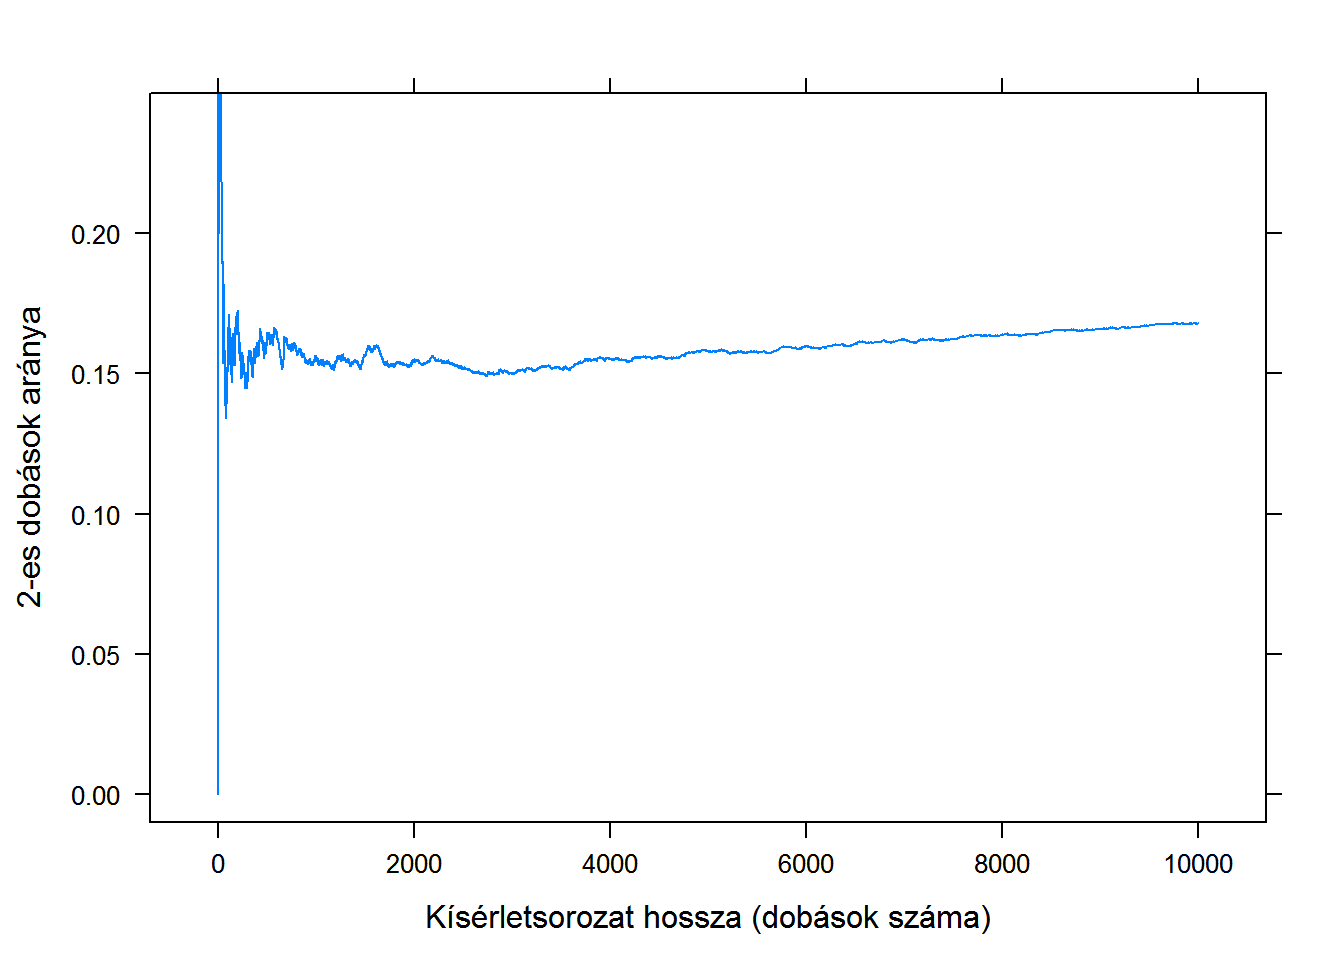
\includegraphics{FerenciTamas_ValszamEsStatAlapvonalai_files/figure-latex/unnamed-chunk-6-1} \end{center}

(Én ezt persze most számítógépen szimuláltam, azonban bármilyen elképesztő, de a hőskorban, a 18. században \emph{tényleg} végrehajtottak ilyen és ehhez hasonló kísérletsorozatokat kézzel, majd ábrázolták az eredményt mint itt!)

Azt látjuk tehát, hogy a relatív gyakoriság, szemben a sima gyakorisággal, nagyon is izgalmasan viselkedik: úgy tűnik, hogy az értéke konvergál valamihez! Ha ezt sokszor megismételjük, akkor mind hasonló képet kapunk, a relatív gyakoriság -- ebben a példában -- \(1/6\)-hoz tart. Fordítva megfogalmazva azt is mondhatjuk: a relatív gyakoriság értéke ingadozik valamilyen érték, mint itt az \(1/6\) körül -- és a frekventista interpretáció azt mondja, hogy ez az érték épp a valószínűség lesz.

Nagyon egyszerűen szólva tehát a frekventista interpretáció a következő: a valószínűség az, amihez a relatív gyakoriság tart! Ennek az interpretációnak később még sok egyéb vetülete is lesz, de számunkra most ennyi elég: a valószínűség absztrakt, matematikai fogalmát hozzáhorgonyoztuk valamilyen tényleges valóságban tapasztalható, fizikai jelenséghez. Hiszen a frekventista interpretáció így azt mondja: ha tudni akarjuk egy esemény valószínűségét, akkor végezzünk egy jó hosszú kísérletsorozatot, számoljuk az esemény relatív gyakoriságát, és nézzük meg, hogy ez mihez tart.

Szabályos kockánál azt fogjuk tapasztalni, hogy minden kimenet azonosan \(1/6\) valószínűségű, és hogy bármely esemény valószínűsége a benne lévő kimenetek darabszáma szorozva \(1/6\)-dal. (Tehát például a páros dobás valószínűsége \(3 \cdot\frac{1}{6}=3/6=1/2\), annak valószínűsége, hogy a dobott szám 5 vagy annál nagyobb \(2 \cdot\frac{1}{6}=2/6=1/3\).)

Ahogy mondtam, a további interpretációkról nem akarok itt beszélni, de talán azért arra érdemes felhívni a figyelmet, hogy miért vannak egyáltalán további interpretációk, milyen problémáig vannak a frekventista iskolának. Egyetlen illusztráció, csak gondolatébresztés gyanánt: teljesen természetesnek vesszük, ha a híradó végén az időjárásjelentés azt mondja, hogy \enquote{30\% a valószínűsége annak, hogy holnap esni fog az eső}. De gondoljuk csak jobban végig, milyen értelemben beszélünk itt valószínűségről? Frekventista értelemben? Azaz ha nagyon sokszor kipróbálnánk, hogy holnap esik-e az eső, akkor a próbák nagyjából 30\%-ában találnánk azt, hogy esik az eső\ldots?

\hypertarget{a-feltuxe9teles-valuxf3szuxednux171suxe9g}{%
\section{A feltételes valószínűség}\label{a-feltuxe9teles-valuxf3szuxednux171suxe9g}}

Bár ez a fogalom csak valamilyen technikai apróságnak tűnhet, valójában egy borzasztó fontos koncepcióról van.

Az alapkérdés az, hogy hogyan tudunk a valószínűségbe valamilyen \emph{ismert információt beépíteni}. Más szóval, \emph{ha} tudjuk, hogy valami megtörtént, akkor ezen információ fényében hogyan módosul események valószínűsége? Hiszen ha van valamilyen részleges információnk, az nagyon is befolyásolhatja a valószínűségét egy eseménynek, például megtudjuk azt, hogy a dobott szám 3 vagy annál kisebb, az módosítja annak a valószínűségét, hogy párosat dobtunk (ahhoz képest mintha nem tudnánk semmit). Az elnevezés nagyon szerencsés, hiszen ezt úgyis kiolvashatuk: \emph{feltéve}, hogy legfeljebb 3-ast dobtunk, mennyi annak a valószínűsége, hogy párosat dobtunk? A matematikusok így szoktak beszélni, de ehhez mindig tartsuk észben, hogy a \enquote{feltéve} szót az előbbi értelmeben kell venni: ha ismerjük azt az információt, hogy legfeljebb 3-ast dobtunk, akkor ennek figyelembevételével, azaz ennek fennállása esetén mennyi a valószínűsége a páros dobásnak. Lényegében az a kérdés, hogy valamilyen állítást igaznak fogadva el (legfeljebb 3-ast dobtunk), erre szorítkozva, tehát leszűkítve a világunkat arra, ahol ez igaz, ezen \emph{belül} mekkora a páros dobás valószínűsége.

Ez a legutolsó megfogalmazás már az utat is mutatja a számításhoz. Nevezzük \(A\)-nak azt az eseményt, aminek a valószínűségére kíváncsiak vagyunk (az előző példában \(A=\left\{⚁,⚃,⚅\right\}\)), \(B\)-nek pedig a feltételét, tehát amiről tudjuk, hogy megvalósult (\(B=\left\{⚀,⚁,⚂\right\}\)). Mi a valószínűsége, hogy párosat dobtunk, feltéve, hogy legfeljebb 3-ast dobtunk? Abban a világban vagyunk, amiben igaz, hogy legfeljebb 3-ast dobtunk, és azt kérdezzük, hogy -- ezen belül! -- mekkora valószínűséggel dobtunk párosat.

A kérdés megválaszolásához legjobb a festővászonra rajzolt pacás analógia, ahol az események a pacák, és a valószínűség pedig az, hogy a paca a vászon mekkora részét teszi ki. (Hiszen a pacának a területét mérjük, mégpedig úgy, hogy 1-nek a vászon területét neveztük.) Mit mondtunk most? Azt, hogy abban a világban vagyunk, amiben a \(B\), a feltétel teljesült, erre szűkítjük magunkat. Ez tehát azt jelenti, hogy a festővászon helyett a világunkat a \(B\) pacára szűkítjük le, és azon \emph{belül} kérdezzük, hogy mekkora \(A\) területe. Mivel ez utóbbi (\(B\)-n belül \(A\) területe) nem más, mint \(A\) és \(B\) közös területe, így a kérdésünk egyszerűen annyi: \(A\) és \(B\) paca közös része \(B\) mekkora részét -- \emph{nem a vászon mekkora részét} -- teszi ki! Ami persze nem más, mint \(A\) és \(B\) közös területe osztva \(B\) teljes területével:

\begin{center}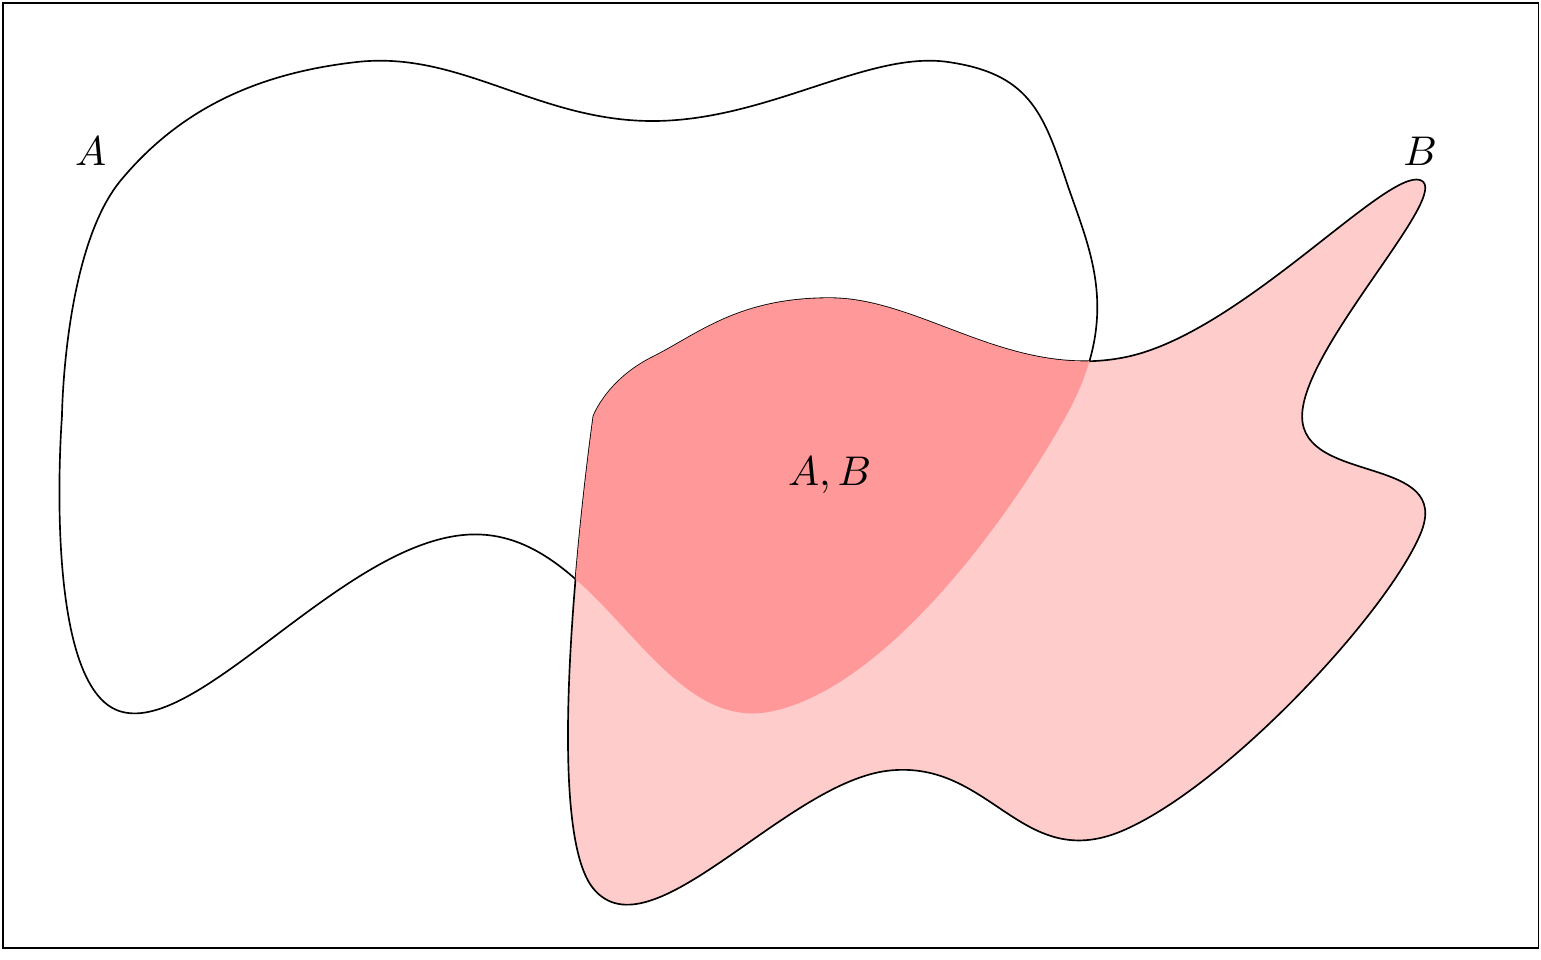
\includegraphics{FerenciTamas_ValszamEsStatAlapvonalai_files/figure-latex/unnamed-chunk-7-1} \end{center}

Így tehát kapjuk a \textbf{feltételes valószínűség} definícióját, melyet úgy jelölünk, hogy \(\mathbb{P}\left(A \mid B\right)\), ahol \(A\) valószínűségét kérdezzük és \(B\) a feltétel:
\[
\mathbb{P}\left(A \mid B\right) = \frac{\mathbb{P}\left(A,B\right)}{\mathbb{P}\left(B\right)},
\]
ahol \(A,B\)-vel jelöltük azt, hogy \enquote{\(A\) és \(B\)} (így a valószínűségüket a \(\mathbb{P}\left(A,B\right)\) jelöli).

Így lehet tehát egy ismert információ (\(B\)) beépítésével úgymond pontosítani egy valószínűséget! \(\mathbb{P}\left(A\right)\) a valószínűség \emph{mielőtt} megtudnánk bármilyen plusz-információt, szokták emiatt ezt \textbf{prior valószínűségnek} nevezni, \(\mathbb{P}\left(A \mid B\right)\) pedig a valószínűség \emph{miután} megtudtuk \(B\)-t, szokták ezt ezért \textbf{poszterior valószínűségnek} nevezni. A feltételes valószínűséggel tehát be tudjuk építeni az új ismeretet valamilyen valószínűségi kérdés megválaszolásába.

Az előbbi példánkat folytatva, szabályos kockánál annak a valószínűsége, hogy \enquote{párosat dobunk és legfeljebb 3-ast dobunk} (\(\mathbb{P}\left(A,B\right)\)) \(1/6\), hiszen az egyetlen kimenet aminél előfordul az a 2-es dobás, és emlékezzünk vissza, hogy szabályos kockánál egy esemény valószínűsége a benne lévő kimenetek darabszáma szorozva \(1/6\)-dal. Annak a valószínűsége, hogy legfeljebb 3-ast dobunk (\(\mathbb{P}\left(B\right)\)) ugyanezen logikával \(3/6=1/2\), így a keresett feltételes valószínűség: \(\frac{1/6}{3/6}=1/3\). A kérdésünket tehát most már meg tudjuk válaszolni: annak a valószínűsége, hogy párosat dobtunk, feltéve, hogy legfeljebb 3-ast dobtunk \(1/3\).

(Észrevehető, hogy az osztásnak nincs értelme, ha \(\mathbb{P}\left(B\right)=0\). De hát ez logikus is: egy 0 valószínűséggel bekövetkező eseménynél nincs sok teteje egy olyan kérdésnek, ami úgy kezdődik, hogy \enquote{feltéve, hogy ez bekövetkezik\ldots{}}.)

A fenti definíciót átrendezhetjük a következő formába: \(\mathbb{P}\left(A,B\right)=\mathbb{P}\left(A \mid B\right)\cdot \mathbb{P}\left(B\right)\). Ez kiolvasva azt mondja, hogy két esemény együttes bekövetkezésének a valószínűsége egyenlő a feltételes valószínűséggel szorozva a feltétel valószínűségével. Persze az együttes valószínűség szimmetrikus (\(A,B\) ugyanaz, mint \(B,A\), hiszen az nyilván mindegy, hogy azt mondom, hogy \enquote{\(A\) és \(B\) is bekövetkezett} vagy azt, hogy \enquote{\(B\) és \(A\) is bekövetkezett}), \(\mathbb{P}\left(A,B\right)=\mathbb{P}\left(B,A\right)\), ezért nyugodtan írhatjuk ezt is: \(\mathbb{P}\left(A,B\right)=\mathbb{P}\left(B \mid A\right)\cdot \mathbb{P}\left(A\right)\).

Külön említést érdemel, ha két eseményre teljesül, hogy \(\mathbb{P}\left(A \mid B\right)=\mathbb{P}\left(A\right)\). Ez magyarán azt jelenti, hogy \(B\) ismerete \emph{nem változtatta meg} \(A\) valószínűségét: az új információ se nem csökkentette, se nem növelte \(A\) fennállásának a valószínűségét. Ilyenkor szokták azt mondani, hogy \(A\) és \(B\) \textbf{független események}\footnote{A valószínűségi értelemben vett függetlenségnek nem feltétlenül van köze a \enquote{függetlenség} hétköznapi értelméhez, mondjuk, hogy az egyik nem okozza a másikat: egyszerűen annyit jelent, hogy \(A\) esemény \(B\)-n belüli területe \(B\)-hez viszonyítva ugyanannyi mint \(A\) egész területe a festővászonhoz viszonyítva.}. A \enquote{páros dobás} és a \enquote{legfeljebb 3-as dobás} tehát \emph{nem} független események: \(1/2\) a valószínűsége annak, hogy párosat dobunk (önmagában, semmi mást nem tudva), de \(1/3\), ha tudjuk, hogy legfeljebb 3-ast dobtunk, tehát erre feltételezünk. A páros dobás valószínűsége tehát megváltozott, a poszterior valószínűsége nem ugyanaz mint a prior valószínűsége. Azonban \enquote{párosat dobunk} és a \enquote{legfeljebb 2-t dobunk} már függetlenek: a legfeljebb 2-t dobtunk ismeretében ugyanúgy \(1/2\) a páros dobás valószínűsége, mint ezen ismeret nélkül.

Helyettesítsük be a függetlenség definícióját a feltételes valószínűség definíciójába: \(\mathbb{P}\left(A \mid B\right) =\mathbb{P}\left(A\right)= \frac{\mathbb{P}\left(A,B\right)}{\mathbb{P}\left(B\right)}\). A második egyenlőségjel két oldalát véve és \(\mathbb{P}\left(B\right)\)-vel beszorozva azt kapjuk, hogy ha két esemény független, akkor \(\mathbb{P}\left(A,B\right)=\mathbb{P}\left(A\right)\cdot \mathbb{P}\left(B\right)\). Független események együttes bekövetkezésének a valószínűsége a külön-külön vett valószínűségeik \emph{szorzata}.

Ebből az alakból még egy dolog látható rögtön. Ha a \(\mathbb{P}\left(A,B\right)=\mathbb{P}\left(A\right)\cdot \mathbb{P}\left(B\right)\) egyenlőség mindkét oldalát \(\mathbb{P}\left(B\right)\)-vel osztjuk le, akkor kapjuk azt, amivel indítottunk, hogy ti. \(\mathbb{P}\left(A \mid B\right)=\mathbb{P}\left(A\right)\). De teljes mértékben jogunkban áll \(\mathbb{P}\left(A\right)\)-val leosztani, ez esetben azt kapjuk, hogy \(\mathbb{P}\left(B \mid A\right)=\mathbb{P}\left(B\right)\). (Ne feledjük, ha egy együttes valószínűséget leosztunk az egyik tag valószínűségével, akkor feltételes valószínűséget kapunk: a másik tag feltételes valószínűségét feltéve azt, amivel leosztottunk.) Tehát a függetlenség \(\mathbb{P}\left(A \mid B\right)=\mathbb{P}\left(A\right)\) definíciója \emph{automatikusan} jelenti azt, hogy \emph{szükségképp} egyúttal \(\mathbb{P}\left(B \mid A\right)=\mathbb{P}\left(B\right)\) -- azaz a függetlenség valószínűségi fogalma \emph{szimmetrikus}, ha az egyik esemény független a másiktól, akkor a másik is független az egyiktől.

\hypertarget{bayesvalszam}{%
\section{A Bayes-tétel}\label{bayesvalszam}}

Egy nagy hírű -- és tényleg rettentő fontos -- tétel fog következni, ami azonban grandiózussága ellenére valójában pofon egyszerűen kihozható, tulajdonképpen csak a feltételes valószínűség definícióját kell kétszer alkalmazni. Egyfelől ugye azt mondtuk, hogy \(\mathbb{P}\left(A \mid B\right) = \frac{\mathbb{P}\left(A,B\right)}{\mathbb{P}\left(B\right)}\), másrészt azt is megállapítottuk -- persze ugyanebből levezetve! --, hogy \(\mathbb{P}\left(A,B\right)=\mathbb{P}\left(B \mid A\right)\cdot \mathbb{P}\left(A\right)\). Tulajdonképpen semmi másra nincs szükségünk, mint hogy összerakjuk a kettőt, a másodikból származó \(\mathbb{P}\left(A,B\right)\)-t beírjuk az első számlálójába:
\[
\mathbb{P}\left(A \mid B\right) = \frac{\mathbb{P}\left(B \mid A\right)\cdot \mathbb{P}\left(A\right)}{\mathbb{P}\left(B\right)}.
\]
És ennyi, ezzel meg is kaptuk a híres-nevezetes \textbf{Bayes-tételt}! A nevét Thomas Bayesről, egy 18. századi angol presbiteriánius lelkészről kapta, aki először alkalmazta ezt az elvet (igaz, írásban csak halál után jelent meg az erről szóló közleménye).

Miért fontos ez a tétel? Rögtön megértjük, hogy mire használható, ha a két végét nézzük: egyik oldalon \(\mathbb{P}\left(A \mid B\right)\) van, a másikon \(\mathbb{P}\left(A\right)\). Mit mondtunk? \(\mathbb{P}\left(A\right)\) az \(A\) esemény valószínűsége anélkül, hogy bármi többet tudnánk, \(\mathbb{P}\left(A \mid B\right)\) pedig a valószínűsége \(B\) ismeretében, tehát beépítve azt az információt, hogy \(B\) megtörtént. Azaz: a Bayes-tétel az, ami \emph{ténylegesen lehetővé teszi egy információ beépítését} a valószínűségbe! Használva a korábban bevezetett szép kifejezéseket: lehetővé teszi, hogy a prior valószínűségekről -- az információ felhasználásával -- áttérjünk a poszterior valószínűségekre.

Később bőven látunk még arra példát, hogy ennek miért van hatalmas jelentősége; most nézzünk illusztráció gyanánt egy nem statisztikai példát!

Legyen \(A\) az, hogy egy vizsgált személy szenved egy betegségben, \(B\) pedig az erre vonatkozó pozitív lelet. Amennyiben az orvosi diagnosztika biztos lenne (ami -- vegyük észre -- azt is jelenti, hogy nem sztochasztikus!), azaz a pozitív lelet azt jelenti, hogy \emph{biztosan} betegek vagyunk, a negatív pedig azt, hogy \emph{biztosan} nem, akkor semmi probléma nincs, és nincsen szükség valószínűségszámításra. Sajnos azonban a legtöbb esetben nem ez a helyzet: a teszt néha még egészséges embernél is pozitív lesz, és néha betegnél is negatív. (Tökéletlen ismeretek, ugyebár!) Az, ha ebben a helyzetben végiggondoljuk a Bayes-tételt, egyúttal egy gyakorlatban is sok meglepetést okozó helyzetre is felhívja a figyelmet.

Nézzünk egy konkrét esetet! A kullancs terjesztette betegségek közül kettő igazán fontos a gyakorlatban, a kullancs terjesztette agyvelőgyulladás és a Lyme-kór. Ez utóbbi lesz kis példánk alanya. A Lyme-kór diagnosztizálása sajnos nem könnyű feladat. Különféle okokból kifolyólag a kórokozó közvetlen kimutatása általában nem lehetséges, ezért ún. szerológiai vizsgálatot végeznek, mely a kórokozó jelenlétére adott immunválaszt igyekszik kimutatni. Sajnos emiatt az egészséges emberek egy részében is pozitív lesz a teszt, például mert korábban átesett fertőzésen, de az immunológiai jelei még nem múltak el, ezt fogja a teszt -- hibásan -- jelenleg is zajló betegségnek hinni. A jelenleg legjobb tesztekkel nagyjából 99\% \enquote{csak} annak a valószínűsége, hogy egy egészséges embernél tényleg negatív leletet ad, tehát az esetek 1\%-ában fordul elő az előbb leírt tévedés. Hasonlóképp, néha az is előfordul, hogy egy beteg embert tévesen egészségesnek minősít, például mert a vizsgálat időpontjában még nem alakult ki az immunválasz, így hiába beteg az alany, a teszt azt fogja hinni, hogy nincs baja. A jelenleg legjobb tesztekkel mintegy 90\% annak a valószínűsége, hogy egy beteg alanynál tényleg pozitív lesz a teszt, 10\% valószínűséggel téved, és a betegnél hibásan negatív leletet ad.

Vegyük észre, hogy ezek a számok mind feltételes valószínűségek! 99\% a valószínűsége, hogy egészséges embert egészségesnek minősít? Ez tehát azt jelenti, hogy feltéve, hogy egészséges az alany, 99\% a valószínűsége, hogy negatív lesz a lelet. Hasonlóképp: 1\% a valószínűsége -- az előbbiből adódóan --, hogy egészséges alanynál tévesen pozitív leletet ad. Ezt pedig úgy mondhattuk volna, hogy jobban látszódjon, hogy mitől feltételes valószínűségről van szó: feltéve, hogy egészséges az alany, 1\% a valószínűsége, hogy pozitív lesz a lelet. 90\%, hogy feltéve, hogy betegek vagyunk pozitív a lelet, és 10\%, hogy feltéve, hogy betegek vagyunk mégis negatív a lelet. Ez tehát mind feltételes valószínűség, ahol arra feltételezünk, hogy igazából mi az állapotunk, és annak a valószínűségét kérdezzük, hogy a lelet milyen lesz.

Ennyi előzmény után nézzük meg a következő javaslatot: \enquote{a biztonság kedvéért érdemes mindenkinek elmennie néha Lyme-kór tesztre, akkor is, ha nincsenek tünetei!}. Első ránézésre nagyon szimpatikus tanácsról van szó: mindannyian tudjuk, hogy mennyire fontos a betegségek megelőzése, ezerszer halljuk, hogy járjunk rendszeresen szűrésekre stb. Ha azonban egy nagyon kicsit utánaszámolunk a dolognak, akkor meglepő dolgokra bukkanunk.

A kérdés: ha pozitív lett a Lyme-kór tesztünk (emlékezzünk vissza, igen kitűnő tesztről van szó, 90\% és 99\% a jósága a két értelemben!), akkor mekkora valószínűséggel vagyunk tényleg Lyme-kórosak? (Borzasztó tanulságos megkérdezni ismerőseinket anélkül, hogy elmesélnénk nekik, hogy miért kérdezzük, csak megkérve őket, hogy \enquote{zsigerből} válaszoljanak.) Az emberek túlnyomó része azt fogja mondani, hogy nagyon valószínű, hogy betegek vagyunk, a legtipikusabb válaszok a 90, meg a 99\% lesznek. Hiszen hát meg is mondtuk, hogy ilyen jó a teszt, akkor most igazából mi ezen a nagy kérdés\ldots?

Számoljunk egy picit! Ahogy mondtuk, legyen \(A\) az, hogy Lyme-kórosak vagyunk, \(B\) az, hogy pozitív lett a szerológiai tesztünk. Mit kérdeztünk, hogy mekkora valószínűséggel vagyunk betegek, ha pozitív a tesztünk? Ez épp \(\mathbb{P}\left(A \mid B\right)\). Az előző okfejtés hibája e ponton azonnal látszik: a 90\% az \emph{nem} ez, hanem az, hogy ha betegek vagyunk akkor mekkora valószínűséggel lesz a teszt is pozitív, tehát \(\mathbb{P}\left(B \mid A\right)\)! Pont a \emph{fordított} irányú valószínűség! Ez tehát hibás, de akkor mi a \emph{helyes} okfejtés? Erre lesz válasz a Bayes-tétel.

Két dologra van szükségünk, az egyik \(\mathbb{P}\left(A\right)\), a betegség prior valószínűsége, tehát, hogy mindenféle tesztelés előtt mennyi annak a valószínűsége, hogy betegek vagyunk. Erre szerencsére most könnyű válaszolni, ha ugyanis megfogadjuk a tanácsot, akkor ez igen jó közelítéssel annyi lesz, mint a betegek aránya az összlakosságon belül, ez ma Magyarországon kb. \(1/1000\). (Miért mondtam, hogy igen jó közelítéssel? Ezt nagyon fontos érteni: a betegek aránya az igazából nem más, mint a betegek relatív gyakorisága -- hány beteg van: gyakoriság, mekkora az arányuk: relatív gyakoriság -- és a magyar lakosság tízmilliós létszáma azt jelenti, hogy itt egy tízmillió hosszú, tehát hatalmas nagy kísérletsorozatot végeztünk, így a relatív gyakoriság már igen közel lesz a valószínűséghez.) Kell még \(\mathbb{P}\left(B\right)\), annak a valószínűsége, hogy a teszt pozitív, semmit nem tudva arról, hogy egészségesek vagyunk-e. Hogyan kapjuk meg ezt? Ehhez egy pici trükköt\footnote{E trükk logikáját \emph{teljes valószínűség tételének} szokták nevezni.} be kell vetnünk: a \enquote{teszt pozitív és egészségesek vagyunk}, valamint a \enquote{teszt pozitív és betegek vagyunk} két kizáró esemény (egyszerre nem állhat fenn mindkettő) így a \enquote{vagy}-gyal összekapcsoltjuk valószínűsége a külön-külön vett valószínűségeik összege. Mi a \enquote{vagy}-gyal összekapcsoltjuk? A \enquote{teszt pozitív és egészségesek vagyunk vagy a teszt pozitív és betegek vagyunk}? Azt, hogy a \enquote{teszt pozitív} azt felesleges kétszer leírnunk az meg, hogy \enquote{betegek vagyunk vagy egészségesek vagyunk} az olyan, mintha nem írtunk volna semmit, tehát összességében ez az, hogy \enquote{a teszt pozitív} -- épp amire szükségünk van! So far, so good, ahogy a művelt francia mondaná, akkor már csak kell annak a valószínűsége, hogy a \enquote{teszt pozitív és egészségesek vagyunk}, meg annak, hogy a \enquote{teszt pozitív és betegek vagyunk}. Nindkettő egy együttes valószínűség, aminek nagyon megörülünk, mert rávágjuk, hogy az pedig nem más, mint a feltételes valószínűség szorozva a feltétel valószínűségével! Tehát annak a valószínűsége, hogy a teszt pozitív és egészségesek vagyunk nem más, mint annak a feltételes valószínűsége, hogy a teszt pozitív feltéve, hogy egészségesek vagyunk (ez tudjuk! 1\%) szorozva annak a valószínűségével, hogy egészségesek vagyunk (\(1-1/1000=0,\!999\)). Teljesen hasonlóan annak a valószínűsége, hogy a teszt pozitív és betegek vagyunk nem más mint annak a feltételes valószínűsége, hogy a teszt pozitív feltéve, hogy betegek vagyunk (90\%) szorozva annak a valószínűségével, hogy betegek vagyunk (\(1/1000\)). Az előbbi szorzat tehát \(0,\!01 \cdot 0,\!999=0,\!00999\), az utóbbi \(0,\!9 \cdot 0,\!001=0,\!0009\), és amint megbeszéltük, a keresett valószínűség egyszerűen e kettő összege: \(\mathbb{P}\left(B\right)=0,\!00999+0,\!0009=0,\!01089\).

És ezzel minden megvan, bevethetjük a Bayes-tételt:
\[
\mathbb{P}\left(A \mid B\right) = \frac{\mathbb{P}\left(B \mid A\right)\cdot \mathbb{P}\left(A\right)}{\mathbb{P}\left(B\right)}=\frac{0,\!9 \cdot 0,\!001}{0,\!01089}=0,\!083.
\]
Az eredmény tehát az, hogy ha pozitív a leletünk, akkor 8,3\% a valószínűsége annak, hogy tényleg betegek vagyunk! Nem 90, meg 99\%, 8,3\ldots! A pozitív leletünk azt jelenti, hogy \emph{még 10\%-ot sem} éri el annak a valószínűsége, hogy tényleg betegek vagyunk!

Az első és legfontosabb ezen eredmény kapcsán, hogy ne úgy tekintsünk rá, hogy itt kijött egy elég megdöbbentő dolog \enquote{valami matematikai hókuszpókusz} eredményeként. \emph{Értsük meg}, hogy mi ennek a megdöbbentő eredménynek az oka! Értsük a jelenség okát, ne fogadjuk el, hogy valami számok ledarálásából ez jött ki, és hát akkor ez van.

Mi a hibás kezdeti benyomásunk oka? Hogy lehet, hogy miközben a teszt kitűnően, 90 meg 99\% jósággal működik, de a pozitív lelet mégis 90\%-nál is nagyobb valószínűséggel azt jelenti, hogy igazából \emph{nem} vagyunk betegek\ldots? Kezdjük az elején: az érdekel minket, hogy ha pozitív a leletünk, mekkora valószínűséggel vagyunk betegek. Ki kap pozitív leletet? Az, aki beteg, és a teszt jól működik nála, meg az, aki egészséges, de a teszt sajnos hibás eredményt ad az esetében. Hány alany jön a kétféle forrásból? Elsőre azt gondolhatnánk, hogy az előbbi lesz a túlnyomó többség, hiszen ha valaki beteg, akkor a teszt 90\% valószínűséggel jól működik nála, míg ha egészséges, akkor mindössze 1\% valószínűséggel lesz hibás. Csakhogy ez hibás logika! A kutya ott van elásva, hogy a betegség ritka, azaz nagyon alacsony a tesztelés előtti valószínűsége annak, hogy betegek vagyunk, mindössze \(1/1000\). Emiatt ezerszer több egészségeset fogunk tesztelni, mint beteget. És ebben van a kulcs: az ezerszer több egészségesnek hiába csak 1\%-a lesz pozitív, de az ezerszer több egészségesnek még az 1\%-a is több, mint az ezredannyi beteg 90\%-a! Ezen múlik a dolog. Kicsi a valószínűsége, hogy egy egészségest elnéz a teszt, de annyival sokkal-sokkal-sokkal több egészségeset tesztelünk, hogy még ezeknek a kicsi hányada is több lesz, mint a helyesen azonosított betegek. Így végeredményben a pozitív leletet kapó betegek többsége helytelenül azonosított egészséges, és nem helyesen azonosított beteg lesz.

Fontos azért azt is látni, hogy nem arról van szó, hogy a teszt rossz. A teszt bizonyos értelemben nagyon is működött: a pozitív lelet \(1/1000\)-ről kb. 10\%-ra, azaz két \emph{nagyságrenddel} emelte annak a valószínűségét, hogy tényleg betegek vagyunk! Az már egy másik kérdés, hogy nagyon alacsonyról indultunk, így az emelés utáni érték is elég alacsony lett.

A példa arra is felhívja a figyelmet, hogy mennyire fontos, hogy ne keverjük össze a feltételes valószínűség irányát, hogy \(\mathbb{P}\left(A \mid B\right)\)-ről vagy \(\mathbb{P}\left(B \mid A\right)\)-ról beszélünk. Amire feltételezünk, az mindig az ismert információ -- hiszen a feltételes valószínűség építi be ezt az információt. Ha ilyen szemmel nézzük a példát, akkor láthatjuk, hogy a 90\% meg a 99\%-os jóságértékek a teszt jósága szempontjából relevánsak, de a gyakorló orvosnak, aki beteget kell, hogy diagnosztizáljon, nem fontosak: az nem érdekes, hogy feltéve, hogy beteg az alany mekkora valószínűséggel pozitív a teszt, hiszen ilyenkor olyasmire feltételezünk, amit az orvosi rendelőben nem tudunk, és annak a valószínűségét kérdezzük meg, amit tudunk! Természetes, hogy ennek pont a \emph{fordítottja} kell, arra kell feltételeznünk, amit tudunk (pozitív a teszt), és annak a valószínűségét kell megkérdeznünk, amit nem tudunk (beteg-e az alany). Ehhez kell a Bayes-tétel, de a fentiből látható, hogy a kettő \emph{nagyon nem} ugyanaz. Azért nem, mert az irány \enquote{megfordításához} bejön a képbe a prior valószínűség.

\hypertarget{a-valuxf3szuxednux171suxe9gi-vuxe1ltozuxf3}{%
\section{A valószínűségi változó}\label{a-valuxf3szuxednux171suxe9gi-vuxe1ltozuxf3}}

\epigraph{A matematikaóra nehéz. Nem megyünk vásárolni?}{\textit{Barbie (1992-es ,,Beszélő Barbie'' kiadás)}}

Az utolsó pont amit meg kell tárgyalnunk, tulajdonképpen a kiindulópont a valószínűségszámítás mélyebb (és matematikailag is intenzívebb) tárgyalásához, itt azonban mégis csak röviden fogunk vele foglalkozni, mert a továbbiakhoz nekünk nem igazán lesz rá szükségünk.

Az alapprobléma a következő: nagyon sokszor jól jön, ha a egy véletlen kísérlet eredményével valamilyen műveletet tudunk végezni. Például szeretnénk beszélni két kockadobás összegéről vagy tíz ember átlagos testtömegéről. Ez első ránézésre nyilvánvaló (ha az egyikkel 2-est dobtunk a másikkal meg 3-ast, akkor az összeg 5), de valójában \emph{nem} az. A probléma, hogy a véletlen kísérlet eredménye az, hogy ⚁ meg az, hogy ⚂ ezeket pedig aligha lehet összeadni! A testtömeges példán talán kevésbé egyértelmű, de ott is erről van szó, a kimenet nem az, hogy 70, hanem az, hogy \enquote{70 kg}. De még világosabb, hogy mi a probléma, ha pénzérmét dobunk fel, ahol a két kimenet \enquote{fej} és \enquote{írás}, szóval ez még felületes szemlélőnek sem érthető úgy, hogy magától működnek a műveletek.

Elvileg persze lehetne mindenféle műveleteket bevezetni a kimenetekre is, de minek? Egyrészt a nulláról kellene ezeket felépítenünk, másrészt minden eseménytérre külön-külön meg kellene tennünk, miközben van egy nagyon jól ismert és jól értett matematikai struktúránk az ilyen műveletek elvégzésére\ldots{} úgy hívják, hogy \emph{szám}. Nem lenne jobb inkább azzal törődni, hogy leképezzük az eseményteret számokra, és ezzel el is van intézve a probléma? Ráadásul így egységesek lehetnénk, hiszen minden eseményteret ugyanarra az objektumra képettük le, a valós számokra.

A dolog nem is tűnik nehéznek: a ⚁-höz rendeljük hozzá azt, hogy 2 (mint szám), a \enquote{70 kg}-hoz azt, hogy 70 (mint szám) , a \enquote{fej}-hez azt, hogy 1 (önkényesen, itt nincs olyan természetesen hozzárendelés) és így tovább. Az ilyen leképezést, függvényt, ami minden kimenethez hozzárendel egy valós számot, \textbf{valószínűségi változónak} nevezzük. A valószínűségi változókat általában az \(X\), \(Y\), \(Z\), \ldots{} betűkkel jelöljük, tehát például egy lehetséges hozzárendelés, hogy \(⚁\mapsto 2\), amit úgy is írhatunk, hogy \(X\left(⚁\right)=2\). (Vigyázat, nincs kapcsos zárójel! Nem az eseményhez, hanem a kimenethez rendelünk számot.) Diszkrét eseménytérnél diszkrét valószínűségi változóról, folytonos eseménytérnél folytonos valószínűségi változóról szokás beszélni.

A valószínűségi változó használatával tehát a kimeneteket leképezzük számokra, amin már jól el tudunk boldogulni. Nagyon fontos, hogy ezzel a \emph{valószínűségeket is átvisszük} a számokra, csak egy kis megállapodást kell tennünk: ha azt mondjuk, hogy mi annak a valószínűsége, hogy \(X=3\), azt úgy értjük, hogy mi azon kimenetekből álló esemény valószínűsége, amely kimeneteket a valószínűségi változó a 3-ba képezi (ami esetünkben egyszerűen a \(\left\{⚂\right\}\) valószínűsége), ha azt mondjuk, hogy mi \(X<3\) valószínűsége, azt úgy értjük, hogy mi azon kimenetekből álló esemény valószínűsége, amely kimeneteket a valószínűségi változó 3-nál kisebb számba képezi (jelen esetben az \(\left\{⚀,⚁\right\}\) esemény valószínűsége) és így tovább. És ezzel kész is vagyunk! Mindenféle ilyen számhalmaznak, tehát adott számnak, több számnak, intervallumnak stb. meg fogjuk tudni adni a valószínűségét. Ezzel \(X\)-re úgy is tekinthetünk mint egy számra, csak épp nem adott számra, hanem egy olyan valamire, ami többféle számot is felvehet értékül -- de nem akárhogy, hanem bizonyos eloszlást követve.

(Egyedül arra kell figyelnünk, hogy a valós számok közül azokhoz akarjunk valószínűséget rendelni, de azokhoz mindegyikhez, amivel tényleg jól tudunk bánni -- mert nem minden számhalmaz ilyen. Ez annyi megkötést jelent, hogy a jól kezelhető halmazokba képeződő kimenetek legyenek megfigyelhető események, hiszen emlékezzünk vissza, a megfigyelhető események halmaza épp az, amihez valószínűséget rendelünk.)

Annak a valószínűségét, hogy a valószínűségi változó egy adott számnál kisebb, tehát \(X<x\) valószínűségét (vigyázzunk a kis- és nagybetűkre! bal oldalon \(X\), tehát a valószínűségi változó van, jobb oldalon \(x\), ami egy általunk megadott tetszőleges valós szám) a valószínűségi változó \textbf{eloszlásfüggvényének} szokták nevezni. Ez csakugyan \(x\) függvénye, hiszen minden \(x\)-hez megad egy valószínűséget. Például szabályos kockadobásnál így néz kis:

\begin{center}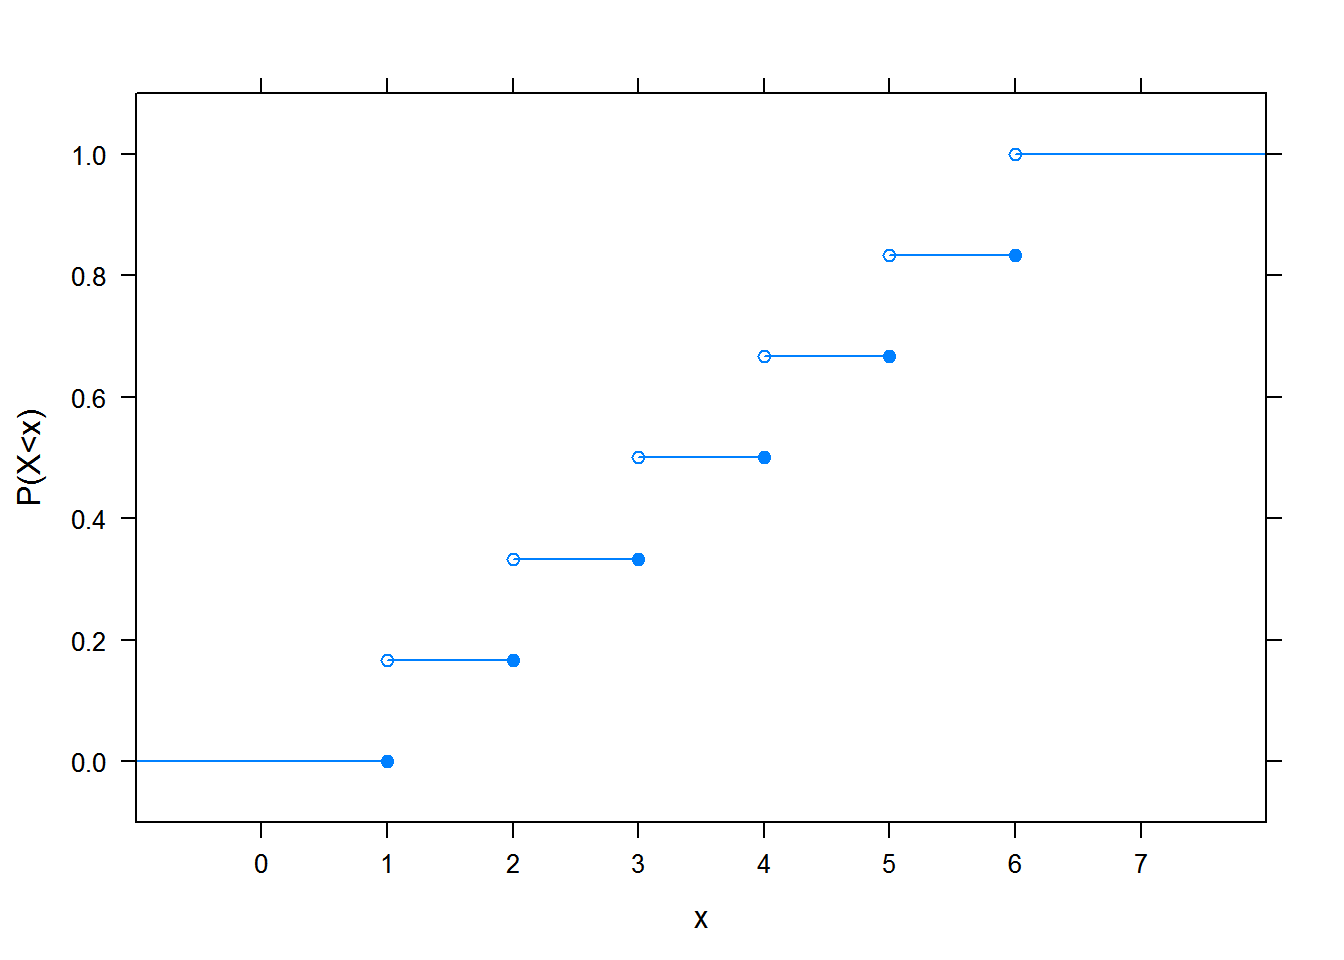
\includegraphics{FerenciTamas_ValszamEsStatAlapvonalai_files/figure-latex/unnamed-chunk-9-1} \end{center}

(Figyeljük meg a nyílt és zárt karikákat! Mivel azt mondtuk\footnote{Ez a magyar -- és az egykori szovjet -- szokás. A nyugati irodalmak gyakran \(X\leq x\) valószínűségével definiálják az eloszlásfüggvényt.}, hogy \(X<x\) valószínűsége érdekel minket, ezért azokat az ábra szerinti módon kellett kirakni, például pont 1-ben még 0 lesz a függvény értéke, hiszen 0 valószínűséggel \emph{kisebb} a valószínűségi változó mint 1.)

Eloszlásfüggvénye minden valószínűségi változónak, diszkrétnek és folytonosnak is van.

Diszkrét valószínűségi változónál azokból az számokból is csak diszkrét sok van, amihez a valószínűségi változó nem nulla valószínűséget rendel, így általában érthetőbb képet ad, ha egyszerűen ezeket ábrázoljuk:

\begin{center}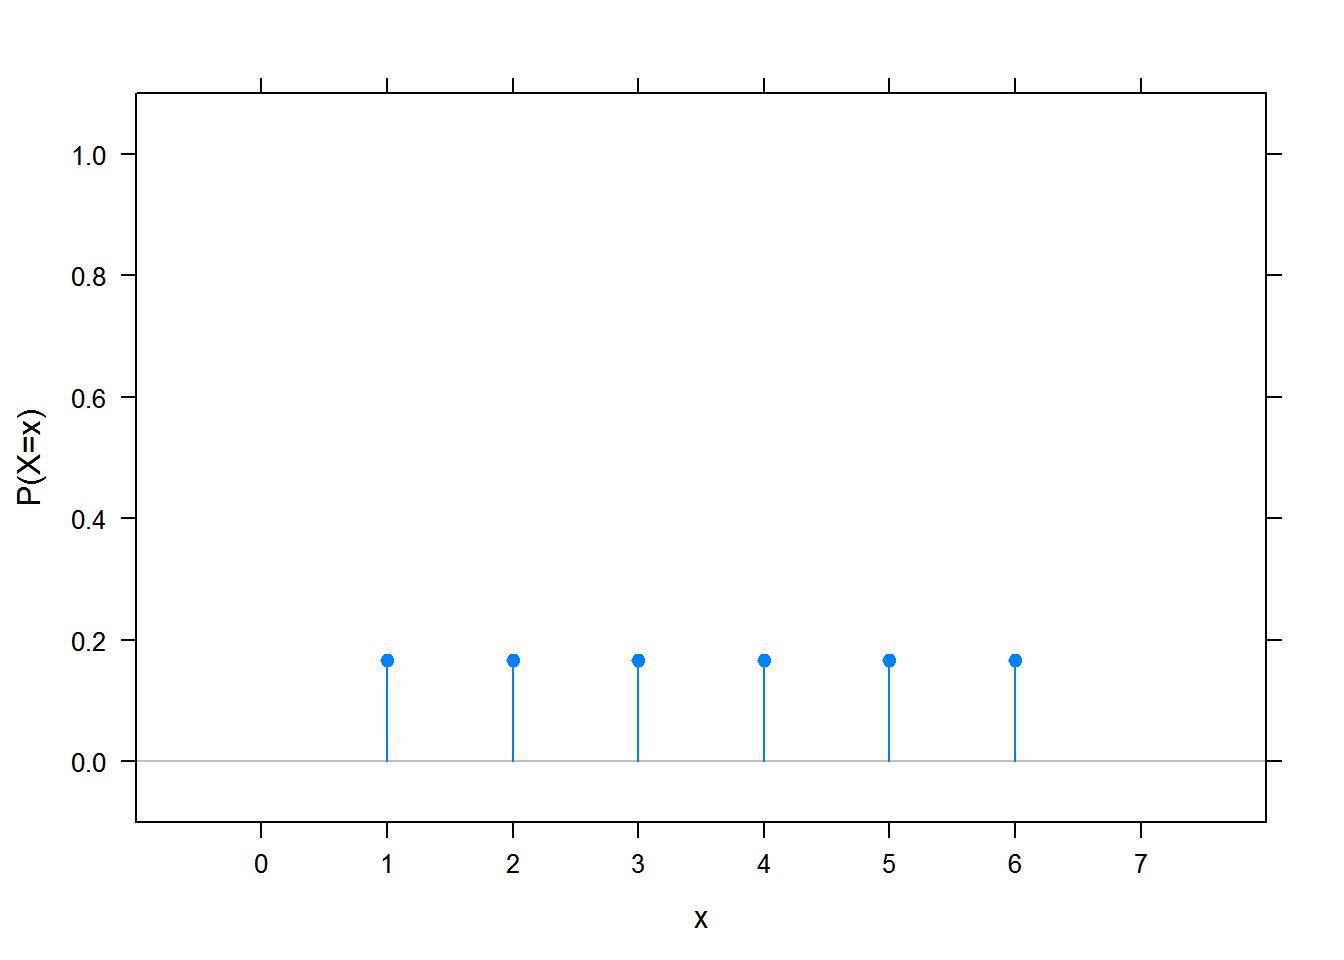
\includegraphics{FerenciTamas_ValszamEsStatAlapvonalai_files/figure-latex/unnamed-chunk-10-1} \end{center}

Ezt szokás a változó \textbf{valószínűségi súlyfüggvényének} nevezni, de sokszor egyszerűen csak azt mondják rá, hogy ez a változó eloszlása.

Folytonos változó esetén zűrősebb a helyzet: be lehet látni, hogy egy folytonos valószínűségi változó minden konkrét értéket 0 valószínűséggel vesz fel! (Ha valakinek ezt nem venné be a gyomra -- miért ne lehetne valakinek a testtömege pont 70 kg? -- az gondoljon arra, hogy a folytonos eset az olyan, mintha végtelen pontosággal mérnénk. Igen, valakinek lehet pont 70 kg a testtömege -- egy kilogramm pontossággal mérő mérlegelen. De ha lecseréljük egy jobb, tized kilogramm pontosságú mérlegre, akkor kiderül, hogy a 70 kg-nak mértek igazából 69,7 vagy épp 70,3 kg-osak. Persze lesz aki még így is 70, azaz 70,0, de ekkor vessünk be egy század kilogramm pontosságú mérleget. Ekkor megint kiderül egy sor emberről, hogy igazából nem 70,00 volt a tömegük. Aki még így is 70,00 marad, azokat lemérjük egy ezred kilogramm pontosságú mérlegen és így tovább. Talán így már jobban elhihető, hogy nulla valószínűségű esemény, hogy valaki 70,0000000\ldots{} kg súlyú legyen, ha a pontossággal a végtelenbe tartunk.) Persze ez nagyon furcsa lehet, hiszen ha minden értéket nulla valószínűséggel vesz fel, akkor meg hogyan lehet, hogy valamilyen értéket mégis 1 valószínűséggel vesz fel\ldots? De a végtelen ilyen furcsa dolgokat produkál: véges sok nulla összege nulla, sőt, végtelen soké is, ha az csak megszámlálhatóan végtelen -- de nem megszámlálhatóan végtelen nulla összege lehet 1!

Folytonos valószínűségi változó eloszlásfüggvénye (ne feledjük, az létezik folytonos változóra is!) nézhet ki például így:

\begin{center}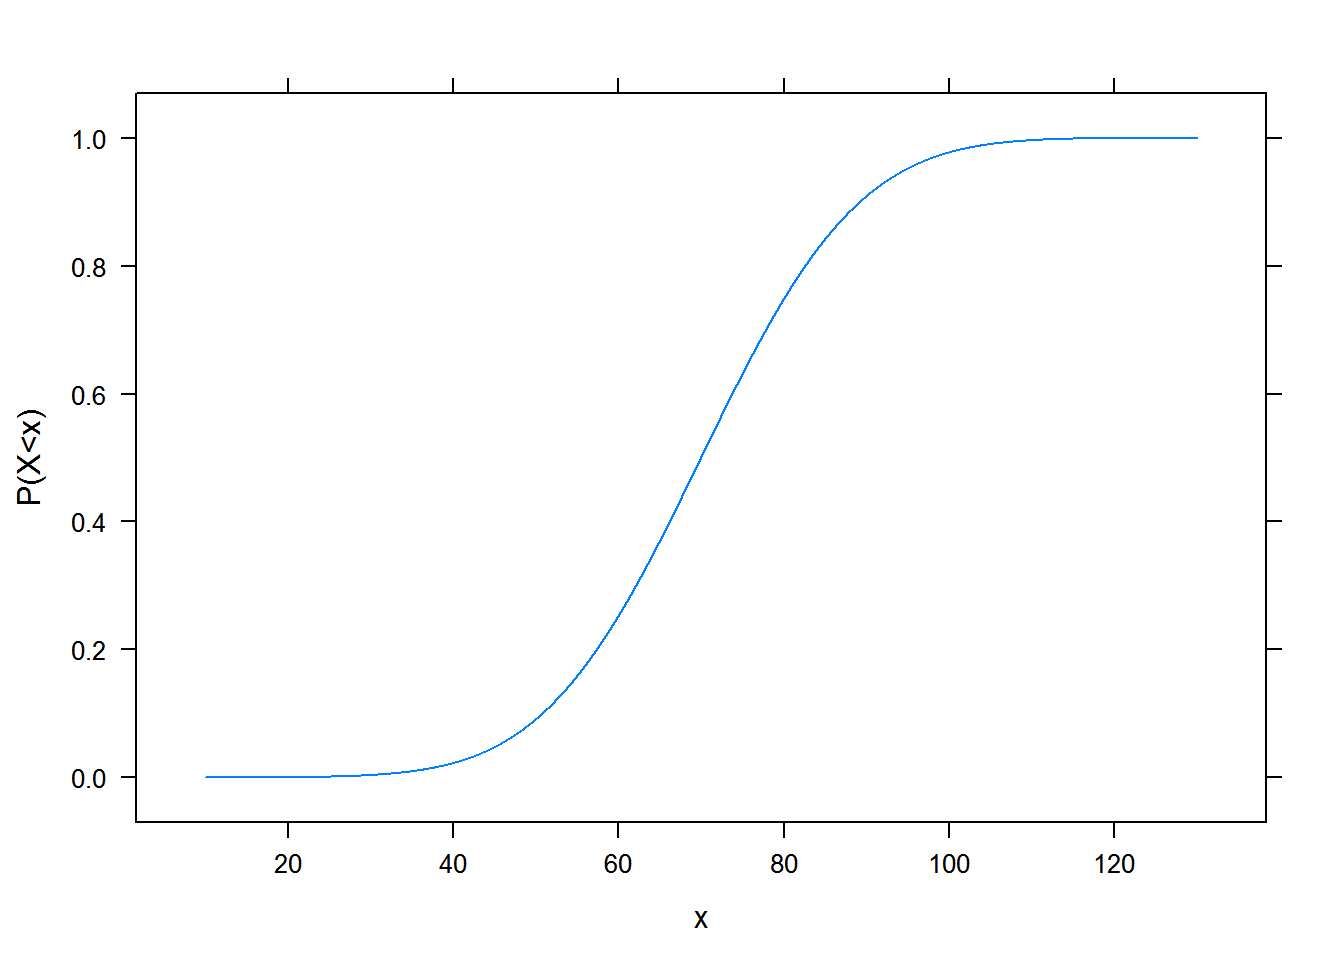
\includegraphics{FerenciTamas_ValszamEsStatAlapvonalai_files/figure-latex/unnamed-chunk-11-1} \end{center}

Folytonos valószínűségi változónál annak tehát nincs értelme, hogy milyen valószínűséggel vesz fel a változó \emph{egy adott} konkrét értéket (mert az minden értékre nulla), de szerencsére annak van értelme, hogy mivel arányos annak a valószínűsége, hogy egy adott érték \emph{kis környezetébe} esik a felvett érték. Ez egyszerű műveletekkel meghatározható az eloszlásfüggvényből; az előbbi esetben így néz ki:

\begin{center}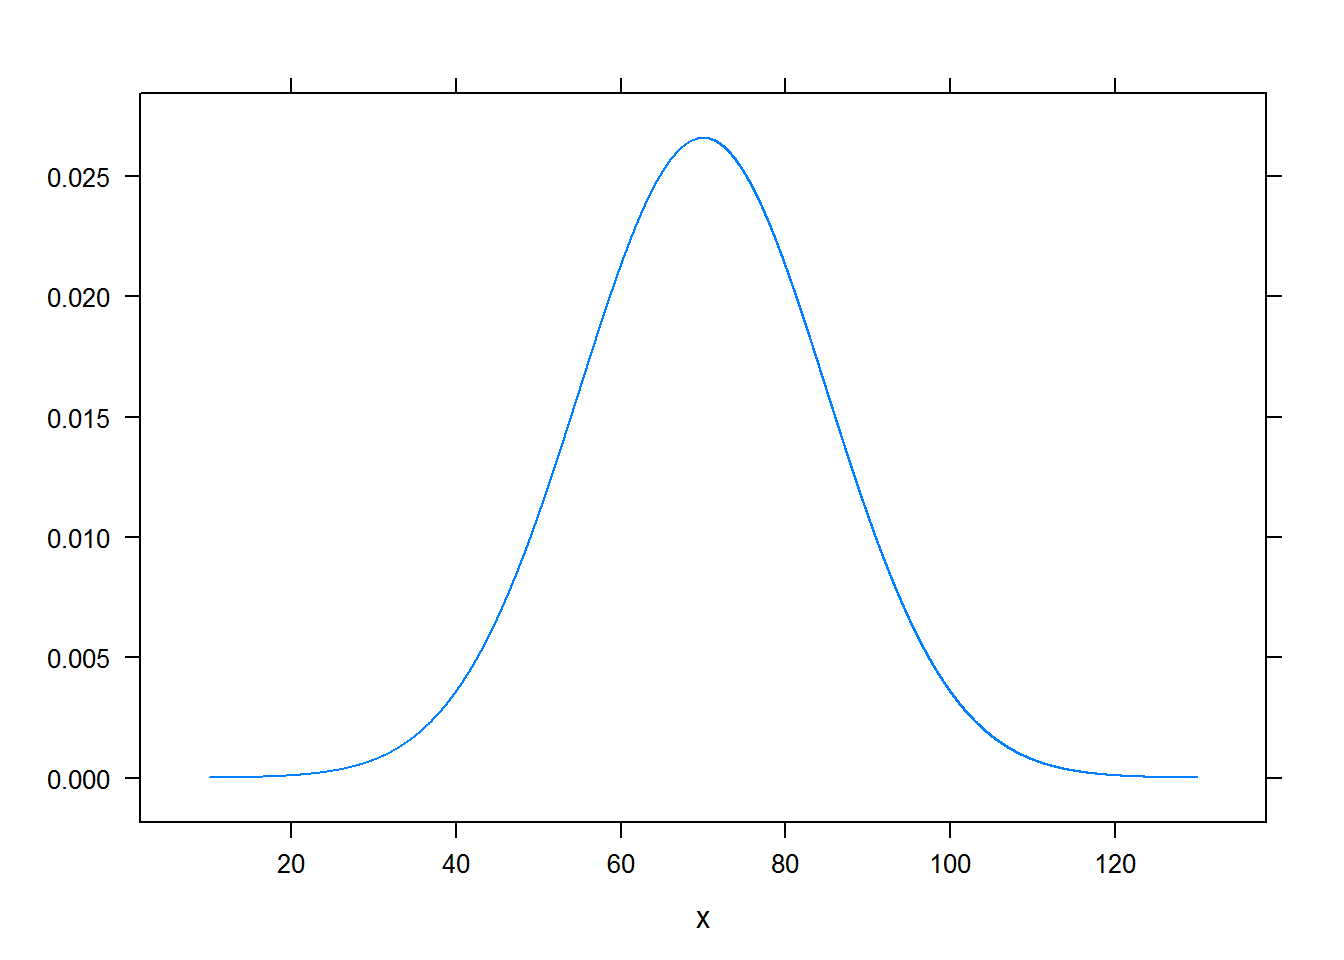
\includegraphics{FerenciTamas_ValszamEsStatAlapvonalai_files/figure-latex/unnamed-chunk-12-1} \end{center}

Olyat nem mondhatunk, hogy ez a valószínűségi változó valószínűbb, hogy 70 értéket vesz fel, mint hogy 40-et (mivel mindkettőt nulla valószínűséggel veszi fel), de olyat a legteljesebb mértékben mondhatunk, hogy valószínűbb, hogy a 70 környékére esik, mint hogy a 40 környékére. Ezt a függvényt szokás a folytonos változó \textbf{sűrűségfüggvényének} nevezni (érzékletes szóval: milyen sűrűn esik a változó egy adott környékre); de itt is gyakori, hogy egyszerűen csak eloszlásról beszélnek.

\hypertarget{a-kuxf6vetkeztetux151-statisztika-alapjai}{%
\chapter{A következtető statisztika alapjai}\label{a-kuxf6vetkeztetux151-statisztika-alapjai}}

A statisztika szó alatt rengeteg dolgot szoktak érteni. Statisztika annak módszertana, hogy hogyan kell az ország inflációját megbecsülni, statisztika, hogy egy piackutatást vagy közvéleménykutatást hogyan kell megtervezni és kiértékelni, statisztika, hogy 10 számból átlagot számolunk, statisztika, hogy 100 számból egy oszlopdiagramot rajzolunk. A statisztika kicsit matematizáltabb területeit két nagy csoportra szokták osztani, leíró (deskriptív) és következtető (induktív) statisztikára. Egyelőre nem mondom meg, hogy ezek a szavak mit jelentenek, mert a szükséges fogalmakat csak később fogom bevezetni, de annyit mindenesetre elárulok, hogy a továbbiakban ez utóbbiról, a következtető statisztikáról lesz szó. (A deskriptív statisztika általában jóval érthetőbb, és sokkal kevesebb kérdést vet fel.)

\hypertarget{egy-ruxe1vezetux151-gyakorlat}{%
\section{Egy rávezető gyakorlat}\label{egy-ruxe1vezetux151-gyakorlat}}

Barátunktól kapunk egy pénzérmét, mely nem feltétlenül szabályos, azaz nem biztos, hogy a fej dobás valószínűsége épp 0,5, azaz 50\%. Lehet bármennyi, jelöljük \(p\)-vel, egyedül annyit kössünk ki, hogy azért nem 0 és nem 1. A kérdés: meghatározni \(p\)-t, azaz megmondani, hogy mekkora valószínűséggel dobunk fejet. Mit csináljuk?

A legtöbben valószínűleg mindenféle statisztikai megfontolás nélkül is azt csinálnák, hogy elkezdik feldobálgatni a pénzérmét, és számolják, hogy hányszor jön ki fej. Mondjuk, hogy 10-szer dobjuk fel, és 7-szor kapunk fejet. Úgy fogjuk mondani: ez lett a mintánk (a minta szó használatának oka később még világosabb lesz). A statisztika azon területét, ami egy megfigyelt jelenségből igyekszik következtetni valamilyen, a jelenség hátterében lévő dologra (jelen esetben a 10 dobásban kapott 7 fejből a \(p\)-re) szokás \textbf{induktív (vagy következtető) statisztikának} mondani.

Mit tudunk tehát mondani a 10 dobásból kapott 7 fej láttán?

\begin{itemize}
\tightlist
\item
  Ettől még a \(p\) \emph{elvileg} akármennyi lehet. Furcsa lenne, ha csak mondjuk 1\% lenne (és mégis 10-ből 7-szer ez jött ki), de nem lehetetlen! Számoljuk is ki, hogy \(p=0,\!01\) mellett mekkora valószínűséggel dobunk 10-ből 7-szer fejet. Ez esetben elsőre 0,01 valószínűséggel dobunk fejet, másodikra szintén, és ha e kettő dobás független egymástól, akkor annak a valószínűsége, hogy elsőre \emph{és} másodikra is fejet dobunk \(0,\!01 \cdot 0,\!01\). (Emlékezzünk vissza, hogy független események együttes bekövetkezésének a valószínűsége a külön-külön vett bekövetkezési valószínűségeik szorzata!) Hasonlóképp, annak a valószínűsége, ha \(p=0,\!01\), hogy az első három fej lesz, nem más mint \(0,\!01^3\), és annak, hogy az első 7 fej lesz, \(0,\!01^7\). Pontosan 7 fejet akkor kapunk, ha a maradék 3 dobás mind írás (\(0,\!99^3\)), így ennek a sorozatnak a valószínűsége \(0,\!01^7 \cdot 0,\!99^3\). Annak a valószínűsége, hogy 10-ből 7-szer jön ki fej azonban ennél jóval nagyobb, hiszen akkor is 7-szer jön ki, ha az első, harmadik, negyedik, \ldots, nyolcadik lesz fej, akkor is, ha az utolsó 7 dobás fej stb. Némi pofozgatás után kiügyeskedhetjük, hogy ennek a valószínűsége: \(0,\!000000000001164\). Hát ez tényleg nem túl nagy\ldots{} de \emph{nem} nulla! Elvileg tehát akkor is dobhatunk 10-ből 7 fejet, ha közben 1\% a fej-dobás valószínűsége.
\item
  Más \(p\) választásnál azonban más lesz annak a valószínűsége, hogy ha annyi az igazi \(p\), akkor mekkora valószínűséggel jön ki 10-ből 7 fej. Például ugyenilyen módon számolva, \(p=0,\!02\)-nél ez \(0,\!000000000144567\), \(p=0,\!1\)-nél \(0,\!000008748\), \(p=0,\!5\)-nél \(0,\!1172\) (egyre nő), \(p=0,\!9\)-nél \(0,\!05740\), \(p=0,\!99\)-nél \(0,\!0001118\) (megint csökken).
\end{itemize}

Lendületbe jöttünk! Akkor már na aprózzuk el, hogy néhány \(p\)-nél számolgatjuk\ldots{} számoljuk ki nagyon sűrűn 0-tól 1-ig és ábrázoljuk, hogy mit kapunk! Íme:

\begin{center}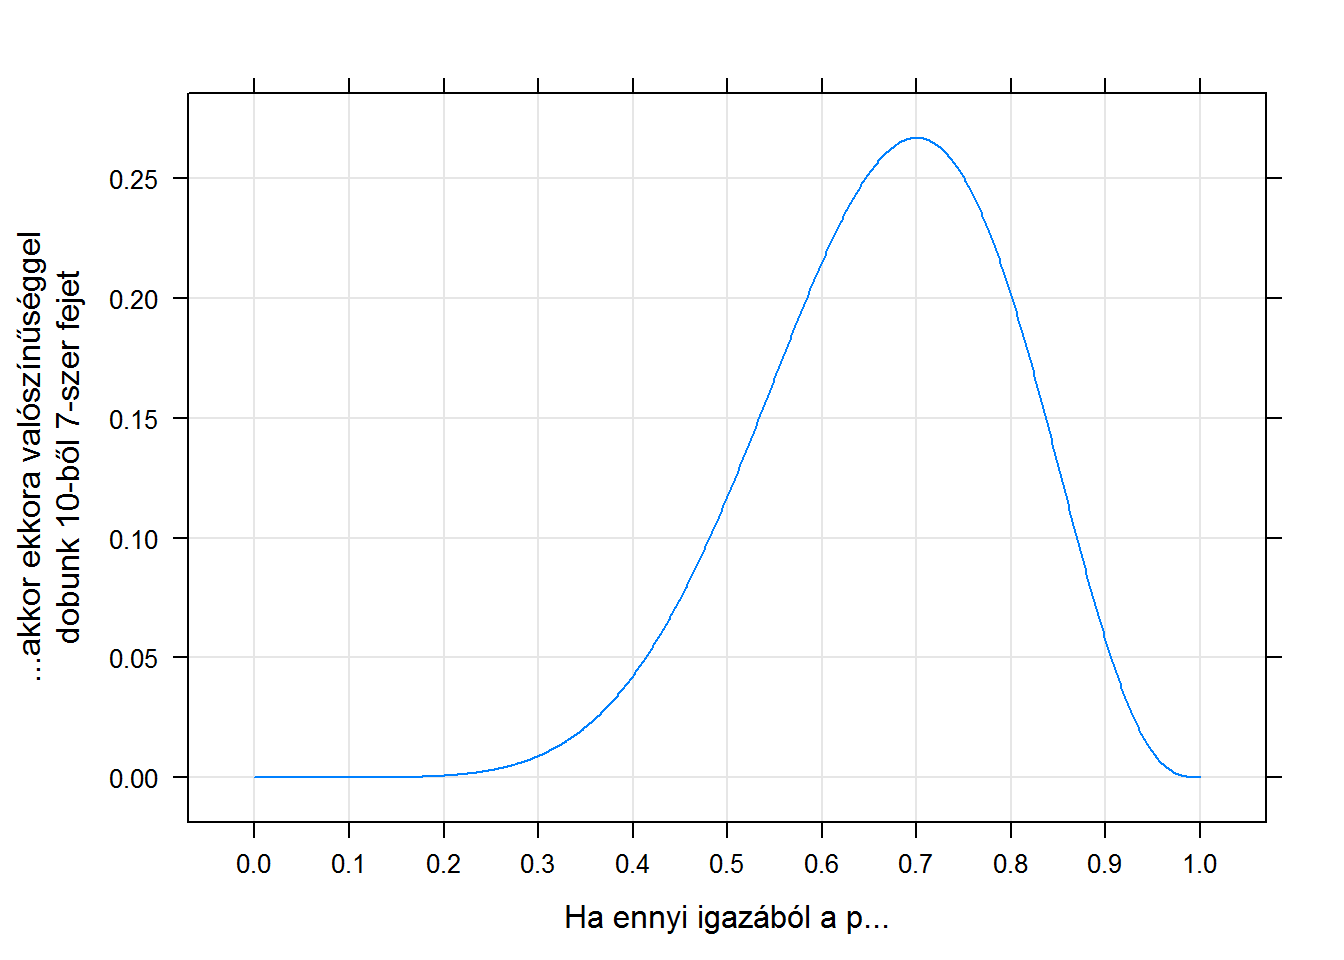
\includegraphics{FerenciTamas_ValszamEsStatAlapvonalai_files/figure-latex/unnamed-chunk-13-1} \end{center}

Azt, hogy \emph{ha} az ismeretlen paraméter valódi értéke egy adott szám lenne, \emph{akkor} mekkora valószínűséggel kapjuk azt, amit ténylegesen kaptunk is, \textbf{likelihoodnak} szokás nevezni. (Most valaki megkérdezhetné, hogy miért nem valószínűségnek hívjuk, hogy egyszer ez egy valószínűség. A kérdés jogos, ebben az esetben nyugodtan hívhatnánk valószínűségnek is, mert a pénzfeldobás kimenete diszkrét. Ha azonban folytonos lenne, akkor is szeretnénk egy ezzel teljesen analóg fogalmat használni, amit azonban semmiképpen nem hívhatnánk valószínűségnek, mert az nem valószínűség, úgyhogy a likelihood szó azért jó\footnote{Felmerül a kérdés, hogy a likelihood-ot hogy mondják magyarul, a válasz: likelihood. A probléma az, hogy a \enquote{valószínűség}-ként való lefordítás konkrétan hibás; próbálkoztak régebben a \enquote{valószerűség} fordítással, de nem igazán ment át a gyakorlatba.}, hogy egy kifejezéssel lehessen egységesen mindkét esetre hivatkozni.) A fenti grafikonon tehát a \enquote{10-ből 7 fej} minta likelihoodja látszik különböző \(p\)-k mellett.

Na most akkor rakjuk össze hol tartunk. Egy: elvileg akármi lehet a \(p\), attól még kaphatjuk azt, amit ténylegesen kaptunk is (10-ből 7 fej)\ldots{} tehát \emph{biztosan} nem tudjuk megmondani, hogy mi a \(p\), bármit is mondunk, az mindenképp tipp lesz. De kettő: igenis tudunk \emph{racionálisan} tippelni, mert hát csak ne tippeljük már azt a \(0,\!01\)-et, ami mellett borzasztó valószínűtlen, hogy 10-ből 7 jöjjön ki\ldots! Miközben épp most jött ki ez ténylegesen! Sőt, menjünk tovább: tippeljük azt, aminek a fennállása mellett a \emph{legvalószínűbb}, hogy az jöjjön ki, ami ténylegesen ki is jött! Tehát ami mellett a legnagyobb a likelihoodja a ténylegesen kijött mintának.

A statisztikusok nem \enquote{tippelést} mondanak, mert az nem sugározza e terület hideg profizmusát, úgyhogy e helyett a -- csakugyan -- sokkal komolyabban hangzó \textbf{becslés} szót használják. Amit a fentiekben láttunk, azt úgy hívják: \textbf{maximum likelihood becslés}, és ezek után már túl sok kommentár nemigen kell hozzá, hogy az elnevezés honnan jön: azt fogadjuk el az ismeretlen paraméter becsléseként, amely mellett a ténylegesen kijött minta likelihoodja a maximális.

Mellesleg ránézve az ábrára, a maximum nagyon úgy tűnik, hogy \(0,\!7\), ami elég gyanúsan pont annyi, mint a fejek aránya a mintánkban\ldots{}

\hypertarget{egy-becslux151fuxfcggvuxe9ny-feluxe9}{%
\section{Egy becslőfüggvény felé}\label{egy-becslux151fuxfcggvuxe9ny-feluxe9}}

\epigraph{Két dolog van, aminél az ember jobb, ha nem látja hogyan készül: a kolbász és a [statisztikai] becslés.}{\textit{Edward Leamer}}

A becslést most megkaptuk egy konkrét mintára. De mi van akkor, ha más a minta? Ha nem 7-szer dobunk fejet, akkor mi lesz a maximum likelihood becslés? Játszunk el egy kicsit a dologgal (azt is beállíthatjuk, hogy hányszor dobtunk):

\begin{center}\href{https://193.224.41.36/shiny/Likelihood/}{\includegraphics{FerenciTamas_ValszamEsStatAlapvonalai_files/figure-latex/unnamed-chunk-15-1} }\end{center}

Eleget próbálkozva valószínűleg mindenkiben kialakul egy benyomás: a maximum likelihood becslés mindig épp a fejek aránya a mintában, tehát a dobálgatásos kísérletsorozatunkban.

Mondom a jó hírt: a dolog nem véletlen. Matematikailag bebizonyítható, hogy ez \emph{mindig} így \emph{kell} legyen: a maximum likelihood becslés az ismeretlen paraméterre (a fej-dobás valószínűségére) a mintabeli arány lesz. Vegyük észre, hogy ezzel egy jóval erősebb eredményt értünk el, mint az előző pontban, hiszen nem \emph{egy konkrét} helyzetre adtuk meg a jó becslést, hanem egy \emph{általános receptet} találtunk, ami \emph{minden} mintára megadja, hogy annál a mintánál mi lesz a jó becslés! A recept tehát egy általános számítási eljárás: megmondja, hogy mit csináljunk a mintában lévő megfigyelésekkel (jelen esetben: számoljuk meg, hogy hány fej van benne, majd osszuk el a dobások számával), hogy megkapjuk az abból a mintából számolható becslést. Az ilyen \enquote{általános receptet} szép nevén \textbf{becslőfüggvénynek} nevezzük. A valószínűség maximum likelihood becslőfüggvénye tehát a mintabeli arány.

\hypertarget{a-bayes-i-probluxe9ma}{%
\section{A bayes-i probléma}\label{a-bayes-i-probluxe9ma}}

\epigraph{Sok nehézséget megspórolnánk, ha [a bayes-i statisztika hívei] követnék Bayes példáját, és csak a haláluk után publikálnának.}{\textit{Maurice Kendall}}

\epigraph{Azt gondolom, hogy van jogos érv a nem bayes-i eljárások használatának védelmében, jelesül, a hozzá nem értés.}{\textit{John Skilling}}

Eddig látszólag minden szép, tiszta és világos. Kézenfekvő a levezetés ahogyan eljutottunk a maximum likelihood becslésig, tökéletesen logikus volt minden lépés. De nézzük csak meg jobban, hogy milyen feltételes valószínűséget vizsgáltunk ott! \(\mathbb{P}\left(\text{minta}\mid\text{ismeretlen paraméter}\right)\). Ha elég sokáig és elég szúrós szemmel nézzük ezt, akkor valószínűleg egyszer csak elfog minket a jeges rémület: a Bayes-tételről szóló részben (\ref{bayesvalszam}. alfejezet) \emph{pont} az ilyen valószínűségek használatával követtünk el kapitális hibát! Hiszen, nézzük meg, pont ugyanaz a baj itt is: arra feltételezünk, amit nem ismerünk, és annak a valószínűségét kérdezzük, amit ismerünk! Ahogy már ott is láttuk, \emph{pont fordítva} kellene: nem az érdekel minket, hogy az ismeretlen paraméter ismeretében mit tudunk mondani a mintáról, hanem az, hogy a minta ismeretében mit tudunk mondani az ismeretlen paraméterről!

Szerencsére épp az ott megtanultak miatt nem esünk pánikba, hiszen tudjuk mi a teendő, hogy megfordítsuk a dolgot, és áttérjünk a \emph{tényleg releváns} feltételes valószínűségre:
\[
 \mathbb{P}\left(\text{ismeretlen paraméter}\mid\text{minta}\right)=\frac{\mathbb{P}\left(\text{minta}\mid\text{ismeretlen paraméter}\right)\cdot \mathbb{P}\left(\text{ismeretlen paraméter}\right)}{\mathbb{P}\left(\text{minta}\right)}.
\]
A számláló első tagja nem probléma: ez épp a likelihood! A nevező szintén nem probléma, a Bayes-tételnél látott trükkel itt is elintézhetjük, ha egyébként a számlálót ismerjük. De mi a helyzet a \(\mathbb{P}\left(\text{ismeretlen paraméter}\right)\)-rel\ldots?

Próbáljuk megérteni, hogy ez mit jelent. Mi a valószínűsége annak, hogy a paraméter adott értékű, \emph{úgy hogy a mintát nem is ismerjük}. Mit gondolunk arról, hogy milyen a fej-dobási valószínűség, még mielőtt egyetlen egyszer is feldobtuk volna az érmét? Valaki esetleg azt mondhatja: semmit, hát épp ezért kezdjük dobálni! Ez egy jogos ellenvetés, de egyelőre rakjuk félre, vagy mondjuk azt, hogy a \enquote{semmit nem gondolunk}, az ezt jelenti\footnote{Van más értelmezése is annak, hogy mit jelent a \enquote{nem tudunk semmit}, de ez félig (nem teljesen!) a filozófia tárgyköre.}:

\begin{center}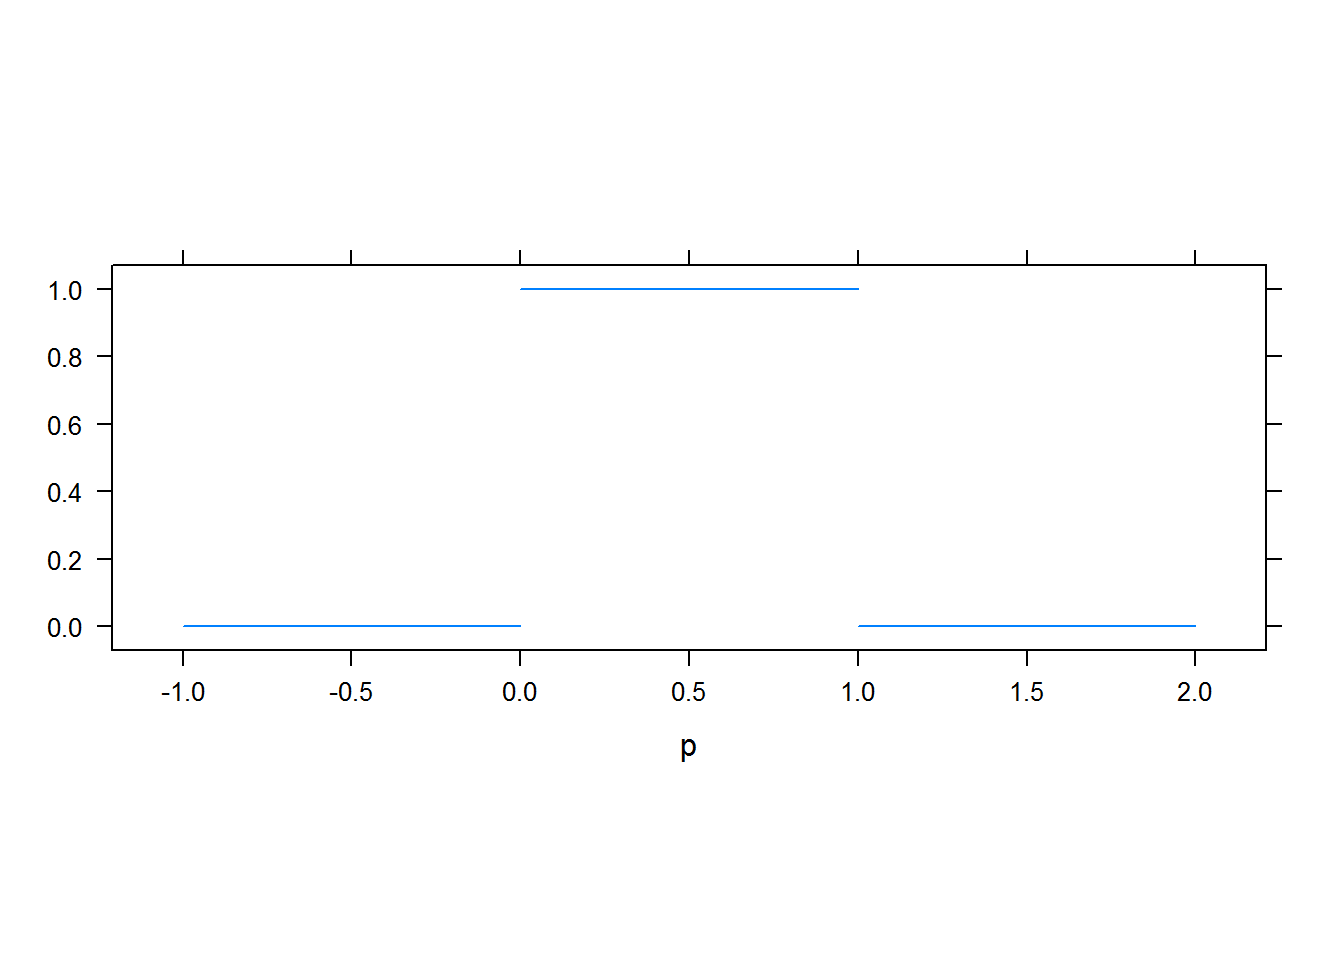
\includegraphics{FerenciTamas_ValszamEsStatAlapvonalai_files/figure-latex/unnamed-chunk-18-1} \end{center}

Tehát: 0-nál kisebb és 1-nél nagyobb nem lehet a fej-dobási valószínűség, azon belül pedig minden érték környékére ugyanakkora valószínűséggel esik\footnote{Ezt szokták \emph{egyenletes eloszlásnak} hívni: bármely 0 és 1 közti intervallumba akkora valószínűséggel esik, mintha az intervallum hossza. Ez tényleg azt jelenti, hogy bármely pont környékére ugyanakkora valószínűséggel esik.}.

Ha azonban jobban megnézzük, akkor most egy nagyon erőteljes eszközt kaptunk a kezükbe. A Bayes-tétel ugyanis lehetővé teszi, hogy \emph{felhasználjuk} ha \emph{van} valamilyen előzetes ismeretünk, elképzelésünk a paraméter eloszlásáról! Például az érmét egy megbízható barátunktól kaptuk, és azt gondoljuk, hogy -- ha nem is biztosan -- de valószínűleg nem cinkelt, legalábbis nem nagyon. Ekkor a következő lehet a feltételezésünk a fej-dobás valószínűségéről, még mielőtt egyetlen egyszer is feldobtuk volna:

\begin{center}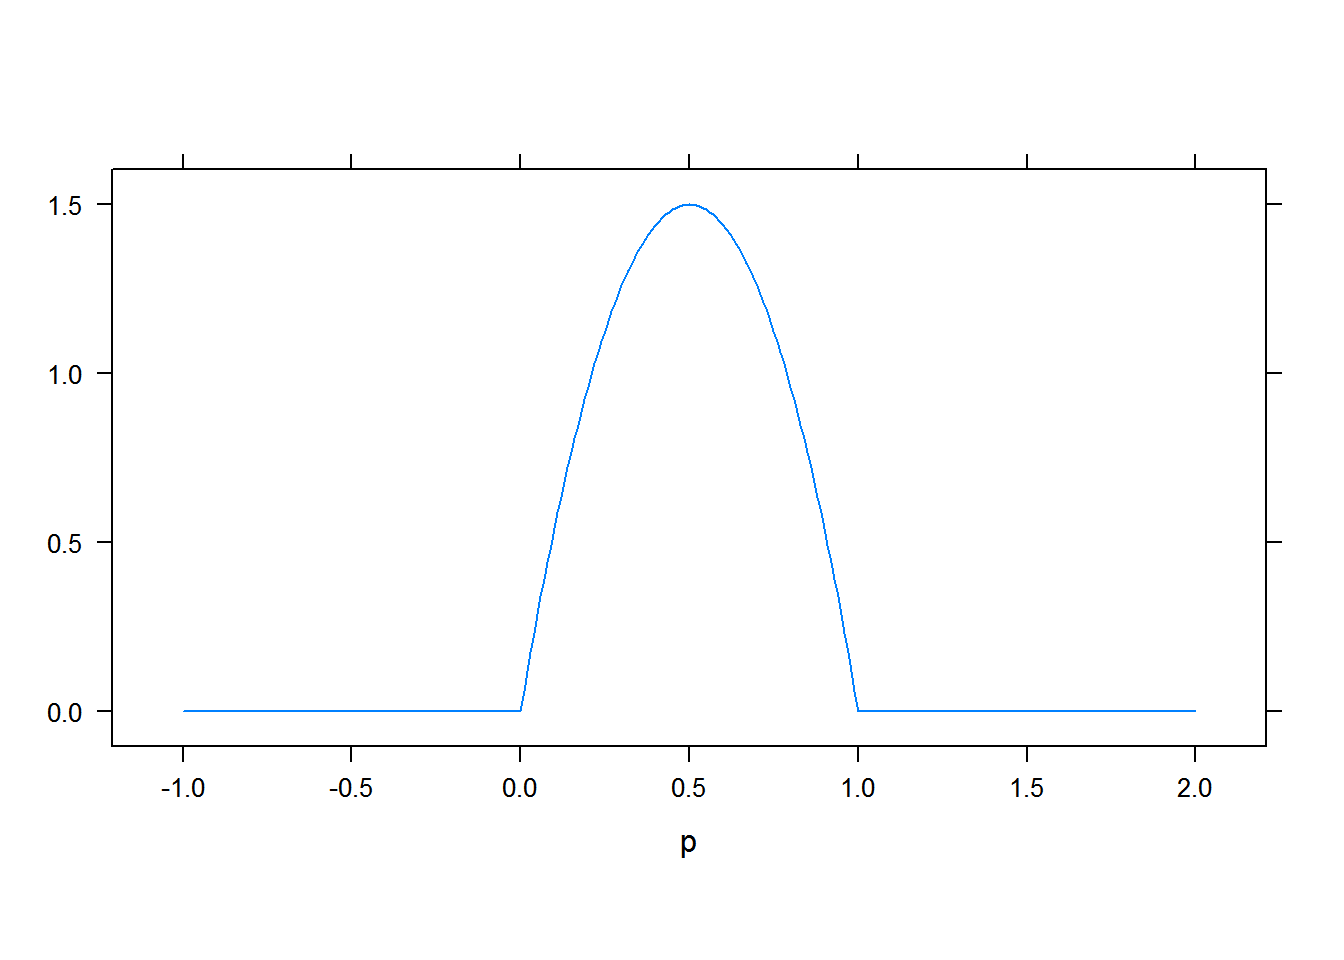
\includegraphics{FerenciTamas_ValszamEsStatAlapvonalai_files/figure-latex/unnamed-chunk-19-1} \end{center}

Ezeket az eloszlásokat szokták -- a korábban mondottak fényében nagyon is érthető szóval -- \textbf{prior eloszlásnak} nevezni.

Mit kapunk a bayes-i megközelítés eredményeként? Korábban azt írtam, hogy \(\mathbb{P}\left(\text{ismeretlen paraméter}\mid\text{minta}\right)\), de ezt némileg idézőjelbe kell tenni: az ismeretlen paraméter egy folytonos dolog (bárhol lehet 0 és 1 között), tehát nem arról lesz szó, hogy mekkora valószínűséggel vesz fel egy értéket, hanem \emph{eloszlása lesz}. Ami tulajdonképpen teljesen logikus: van egy eloszlása a kísérletezgetésünk előtt (a prior eloszlás), és egy másik a kísérletezés után. Hát persze: a Bayes-tétel, amint láttuk, beépít egy információt, és itt is ez történt: fogja a prior eloszlást, beleépíti az információt, ami kiderült a kísérletezésünkből, tehát a mintából, és kiköp egy \enquote{frissített} eloszlást, ami már a minta információját is tartalmazza. Ezt szokás -- szintén logikus szóval -- \textbf{poszterior eloszlásnak} nevezni.

Például egyenletes prior esetén a következő lesz a poszterior (továbbra is mondjuk, hogy 7 fejet dobtunk 10 kísérletből):

\begin{center}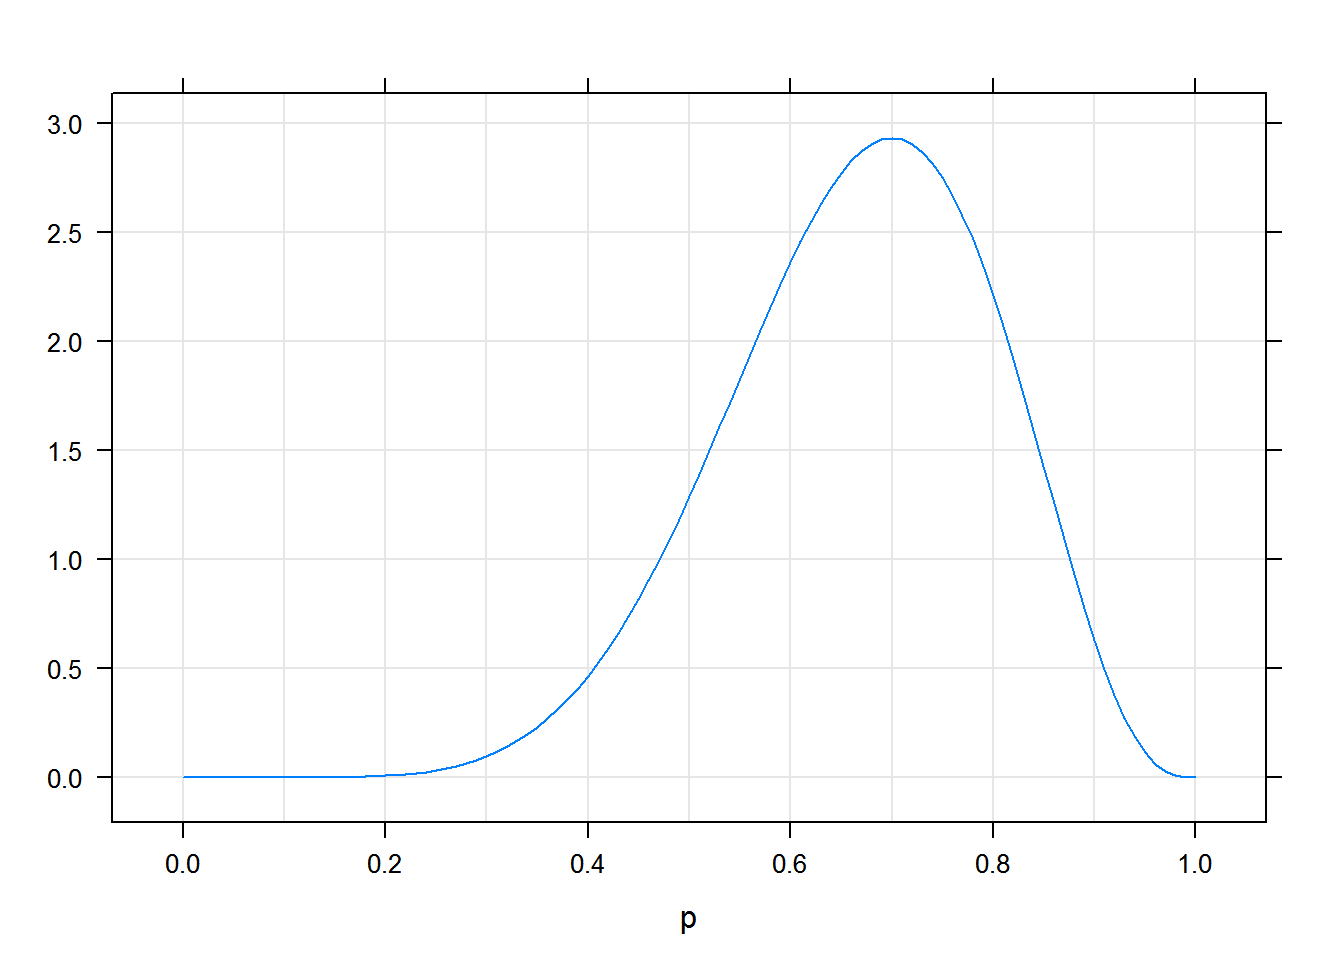
\includegraphics{FerenciTamas_ValszamEsStatAlapvonalai_files/figure-latex/unnamed-chunk-20-1} \end{center}

Viszont a \enquote{baráttól kaptunk a pénzérmét} prior esetén így fog kinézni a poszterior \emph{pontosan ugyanazon minta} mellett:

\begin{center}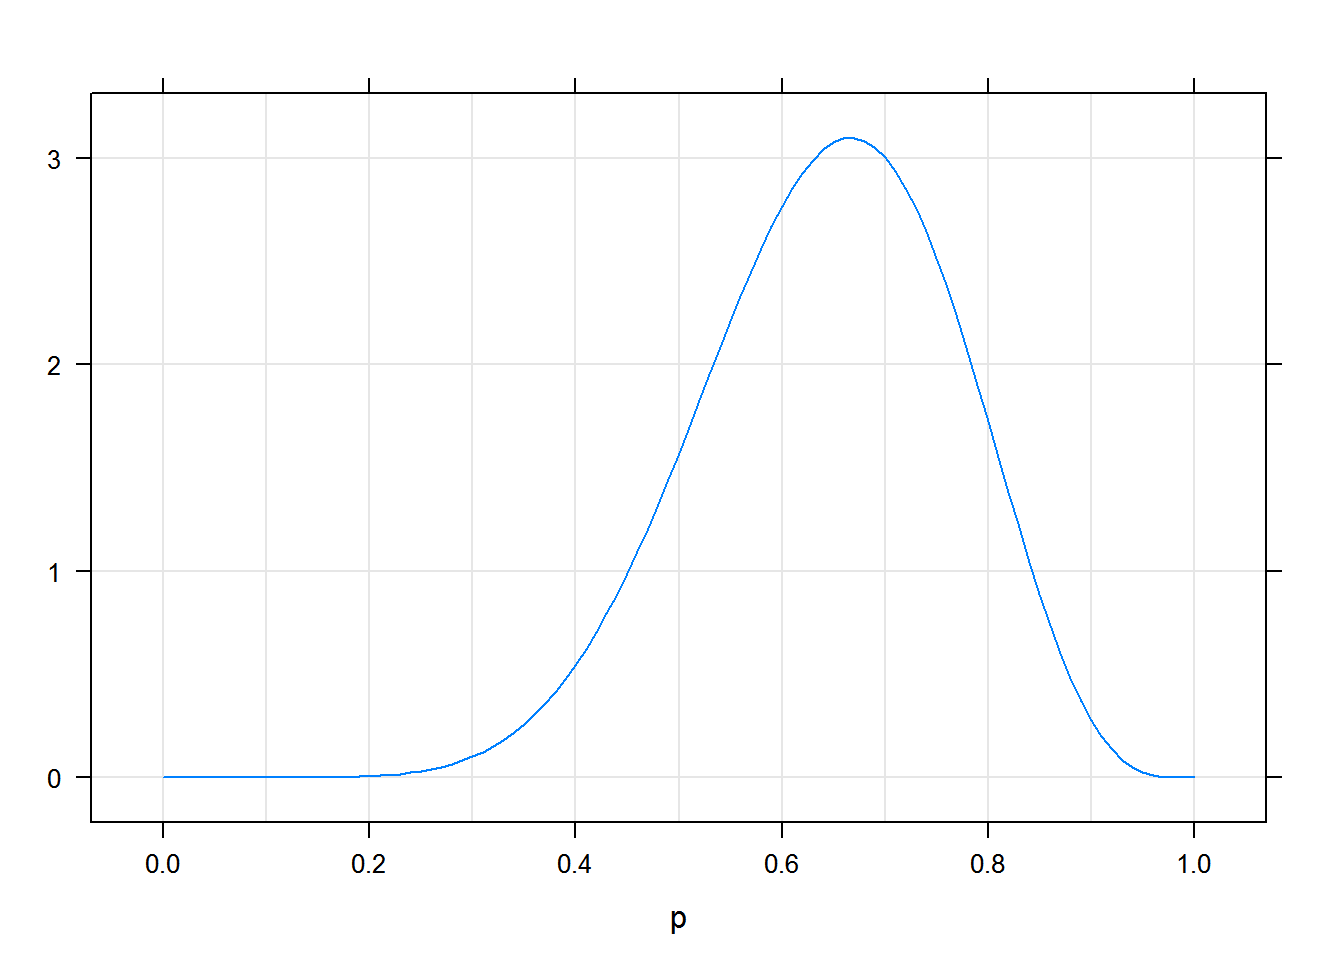
\includegraphics{FerenciTamas_ValszamEsStatAlapvonalai_files/figure-latex/unnamed-chunk-21-1} \end{center}

A különbség nem nagy, de ha jobban megnézzük azért érzékelhető: az utóbbi esetben kicsit balra mászott a poszterior eloszlás. Miért? Azért, mert hiába láttuk azt, hogy a kísérletben meglehetősen cinkeltnek mutatkozott a pénzérme, de mi hajlunk arra egyéb (értsd: kísérletünkön kívüli) okokból, hogy a pénzérme nem annyira cinkelt, ezért bár a próbálkozásunk eléggé meggyőzött az ellenkezőjéről, de nem tökéletesen (nem annyira, mintha nem lett volna ilyen előzetes hiedelmünk). Tehát pontosan azt látjuk, hogy az előzetes ismeret \emph{beleépült} a becslésbe!

Nagyon tanulságos kipróbálni mindenféle prior és minta mellett, hogy hogyan alakul a poszterior, és hogy az hogyan viszonyul a -- prior információval nem törődő -- maximum likelihood becsléshez. A következő grafikonon a két eloszlás mellett látható a maximum likelihood becslés is, vastagabb függőleges vonallal megjelölve (azzal ne törődjünk, hogy az \(\alpha\) meg a \(\beta\) mit jelent, a lényeg, hogy ezek állításával a prior eloszlás alakját nagyon sokféle kinézetre beállíthatjuk):

\begin{center}\href{https://193.224.41.36/shiny/BayesBecsles/}{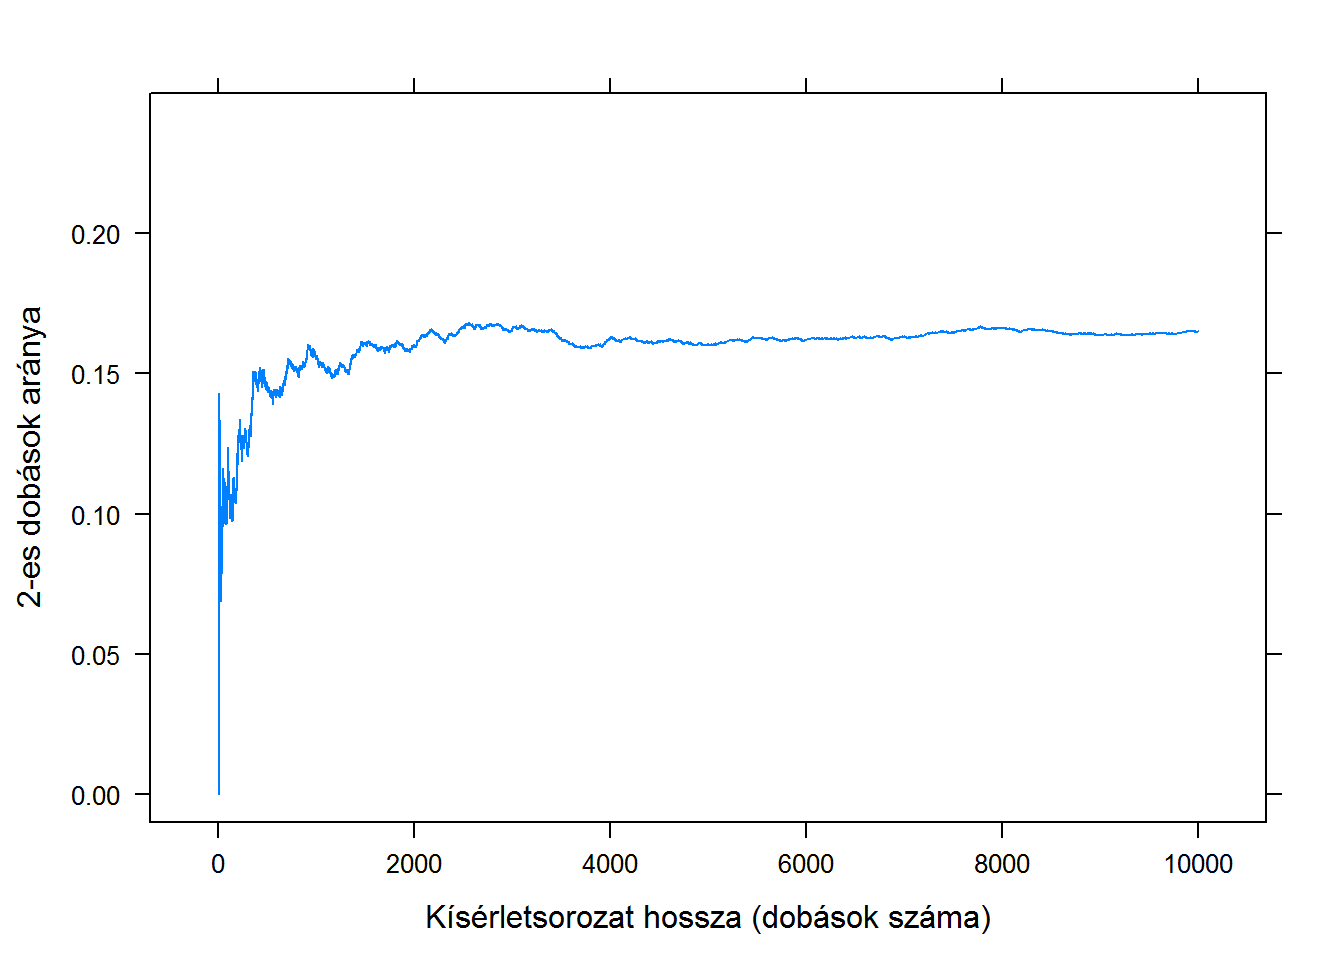
\includegraphics{FerenciTamas_ValszamEsStatAlapvonalai_files/figure-latex/unnamed-chunk-22-1} }\end{center}

Próbálkozzunk mindenféle priorokkal (egyenletes, valahol csúcsosabb) és különböző mintákkal is (nem csak különböző fej-dobás számok, de különböző kísérlethosszak is)!

Milyen tanulságokat szűrhetünk le ebből? A legfontosabbak:

\begin{itemize}
\tightlist
\item
  A prior maga felé \enquote{húzza} a poszteriort, ahhoz képest mint ahol a maximum likelihood becslés lenne. Ennek magyarázatát már láttuk: a poszterior egyszerre veszi figyelembe a prior információt és a dobálgatásunk kimenetét (míg a maximum likelihood becslés csak ez utóbbit).
\item
  Minél csúcsosabb a prior, ez annál inkább igaz. Persze: a csúcsosabb prior azt jelenti, hogy biztosabbak vagyunk már eleve is abban, hogy ott van a paraméter értéke, kevésbé \enquote{bizonytalanít el} minket ebben még egy ellentmondó eredmény is.
\item
  És a végére még egy nagyon fontos dolog: a prior annál jobban számít, minél kisebb volt a minta, tehát minél kevesebbszer dobtuk fel a pénzérmét. De gondoljuk meg, ez kristálytisztán logikus: rövidebb kísérlet kevesebb információt jelent (bármi is jön ki belőle), tehát érthető, hogy az kevésbé befolyásolja az előzetes meggyőződésünket -- ilyenkor még a poszteriort a prior dominálja. De ha nagyon hosszú a kísérletünk, akkor már perdöntő ami abból kijön, kevéssé számít, hogy előzetesen hogyan vélekedtünk. A bayes-i módszertan tehát automatikusan megvalósítja ezt az átmenetet.
\end{itemize}

Felmerül még a kérdés, hogy a bayes-i megközelítésből mégis hogyan kapunk becslést, azaz egyetlen számot, mint amit tippelünk az ismeretlen értékre? Hiszen úgy tűnik, hogy itt csak komplett eloszlásunk van! Valóban, valahogy a legvégén az eloszlásból egyetlen számot kell gyártani. Erre többféle módszer is van, itt most nem tárgyalom részletesen\footnote{Azért az okát elmondom: ahhoz, hogy megmondjuk, hogyan gyártunk az egész eloszlásból egyetlen számot, szükség van \emph{még egy} döntésre: meg kell határoznunk, hogy adott tévedést, hogy a tippelt érték mennyire ment a valós mellé, milyen súlyosnak minősítjük. Például ha kétszer távolabb vagyunk a valóságtól, az kétszer nagyobb baj? Vagy négyszer? Vagy ugyanakkora baj, mert csak az számít, hogy nem találtuk el? Ha erre a kérdésre válaszolunk, akkor abból már kiadódik a becslőfüggvény.}, csak az érzékeltetés kedvéért: olyan megoldások lehetségesek, mint hogy vesszük azt az értéket, ahol a poszterior eloszlás maximuma van, vagy egyszerűen vesszük az egész eloszlás várható értékét.

És ezzel végeztünk! Felépítettük a becsléselméletet \textbf{bayes-i} alapokon is.

A kérdés már csak egy: melyik a jobb? A maximum likelihood jellegű megközelítés, vagy a bayes-i? Ez a probléma a 20. század közepén, második felének az elején merült fel csak (noha a Bayes-tétel 200 évvel korábbi), de akkor viszont nagyon is intenzív formában: a bayes-i megközelítést a statisztikusok egy kisebb, de nagyon elszánt része képviselte, akik elég elsöprő elutasítással találkoztak a többiek részéről, aminek az eredménye egy párját ritkitóan harcias tudományos összeütközés lett a két iskola hívei között.

Ebben a vitában nagyon sok részletkérdés van, de a legfontosabb probléma egyszerű: a priorok ügye. Sok ember gyomra nagyon-nagyon(-nagyon-nagyon) nehezen veszi be, hogy ahhoz, hogy eredményt kapjunk, kell valamit mondanunk arról, hogy mit gondolunk még mielőtt egyáltalán belefogunk a kísérletbe\ldots{} \enquote{Hát én szeretnék csak a kísérlet alapján választ kapni!} \enquote{Pont azért csináltam a kísérletet, hogy megtudjam mi a helyzet!} A bayes-i megközelítésben ezt nem lehet, és nem azért, mert nem vagyunk elég ügyesek, hanem mert ez elvileg lehetetlen, hiszen ebben a megközelítésben a kísérlet csak \emph{módosítja} a hiedelmünket. Ez nem objektív! -- mondják sokan. Hiszen az az objektív, ami magából a kísérletből kijön, és pont, az alapján kell nyilatkozni, az egy teljesen megfoghatatlan szubjektív dolog, hogy én mit mondok mi volt az előzetes elképzelésem\ldots{} hát mondhatok akármit! És hogy ezen múljon a végeredmény?!

Persze, másik oldalról ott van, hogy a bayes-i eljárás ad választ az \emph{igazi} kérdésre. Nem a fordított valószínűséget nézi, hanem azt, ami tényleg releváns számunkra. Ennek az ára az, hogy kell a prior. Ami az objektivitást illeti, a bayes-i módszer hívei erre azt mondják, hogy a maximum likelihood jellegű megközelítésben nincs kevesebb szubjektivitás, csak az el van rejtve különféle részletekben (például a mintavétel jellegének meghatározása), és akkor már jobb, ha ez explicite megjelenik.

E helyütt természetesen nem fogok igazságot szolgáltatni ebben a kérdésben. Két feladatot érzek fontosnak, az egyik -- ami a fentiekben megtörtént -- bemutatni a bayes-i gondolkodást is mint egyenrangú alternatíva, mert ez sok irodalomban vagy nem jelenik meg, vagy csak a másik megközelítés nagyon részletes ismertetése után. Látni kell, hogy jelenleg a legtöbb statisztikai területen a másik iskola dominál, így bármit is gondolunk róla, a második feladat azt részletesen bemutatni, hiszen abban a szellemben íródott cikkeket kell túlnyomó többségben megérteni (és, ha úgy adódik, jellemzően írni is).

\hypertarget{a-frekventista-statisztika-uxe9puxedtmuxe9nye}{%
\section{A frekventista statisztika építménye}\label{a-frekventista-statisztika-uxe9puxedtmuxe9nye}}

\epigraph{Az egyetlen mód, hogy érthetővé tegyük a frekventista eljárásokat az, ha hazudunk róluk.}{\textit{Frank Harrell}}

Először kezdjük gyorsan egy terminológiai kérdéssel: amit korábban többször is úgy hívtam, hogy \enquote{maximum likelihood jellegű} megközelítés, az hivatalos nevén a \textbf{frekventista} megközelítés. Ha valaki arra asszociál, hogy ilyenről már volt szó, a valószínűség interpretációi kapcsán (\ref{valinterpretacio}. alfejezet), akkor hamar ki fog derülni, hogy ez egyáltalán nem véletlen.

Ahogy a korábbiakból is kiderült, a frekventista hozzáállás legfontosabb komponense két szóban összefoglalható: \emph{fordított logika}. Nem azt nézzük, hogy feltéve a mintát mit tudunk mondani valami ismeretlen dologról, hanem azt, hogy feltéve az ismeretlen dolgot, mit tudunk mondani a mintáról. \emph{Ez minden frekventista eljárás sajátja!}

Hogy ezt mélyebben megértsük, kapirgáljuk meg kicsit jobban a maximum likelihood becslőt a pénzfeldobásos példában. Megbeszéltük, hogy ekkor az ismeretlen \(p\) paraméter, az érme ismeretlen fej-dobási valószínűsége a kísérletben kapott fej-dobási aránnyal becsülhető maximum likelihood módon. Azt is megjegyeztük, hogy ez persze csak tipp, hiszen biztosak soha nem lehetünk. Nézzük meg az utóbbit kicsit közelebbről! Mondjuk, hogy ismerjük a \(p\)-t (fordított logika!), és nézzük meg, hogy ekkor a mintabeli arány hogyan viselkedik! Például legyen a \(p=0,\!6\), ekkor mekkora valószínűséggel dobunk 10-ből 0 fejet, 10-ből 1-et, 10-ből 2, \ldots, 10-ből 10-et. A számítást már láttuk is a fejezet elején, csak most nem különböző \(p\)-kre számítjuk ugyanazt a fej-dobás számot, hanem ugyanarra a \(p\)-re különböző fej-dobás számokat. Íme az eredmény:

\begin{center}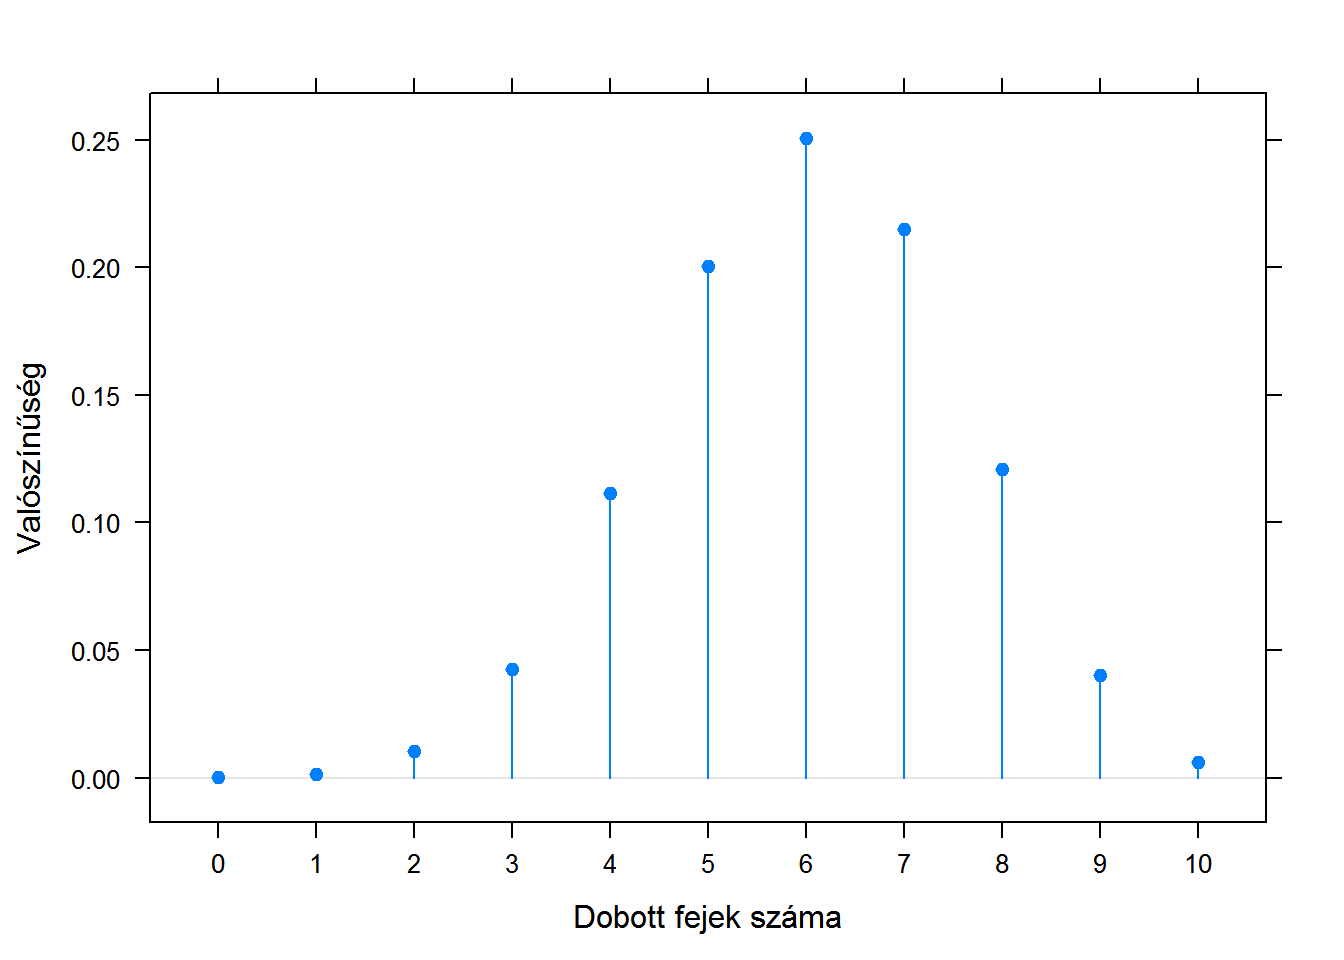
\includegraphics{FerenciTamas_ValszamEsStatAlapvonalai_files/figure-latex/unnamed-chunk-24-1} \end{center}

Tehát még egyszer, ha \(0,\!6\) az ismeretlen paraméter valódi értéke, így fog eloszlani, hogy mi mennyit becsülünk rá a mintából! Látszik, hogy ha pechünk van, akár nagyon eltérhetünk, becsülhetünk akár 20\%-ot, vagy 100\%-ot is -- de ezeknek kicsi a valószínűsége. De ami még fontosabb: meg tudjuk mondani, hogy mennyi!

De egy pillanatra álljunk is meg itt rögtön. Mi az, hogy mekkora valószínűséggel dobunk 2 vagy 10 (vagy akárhány) fejet? Itt van az asztalon a pénzérme, épp most dobtam vele 7-szer fejet, akkor meg miről beszélek, hogy mekkora valószínűséggel dobok 2-szer fejet?! Hát 0, mert 100\% valószínűséggel 7-et dobtam\ldots! Itt jön a frekventista iskola kulcsgondolata: a valószínűségek csak úgy kapnak értelmet, ha \emph{képzeletben újra meg újra megismételnénk} a kísérletünket! Felvenném a pénzérmét (\emph{ugyanazt}! tehát \(p\) ugyanannyi!) és \emph{újra} megcsinálnám a 10 dobásos kísérletet. Feljegyzem, hogy hány fej lett, majd megint megismétlem. Majd megint. Majd megint. Majd megint. Aztán amikor nagyon sokszor megtettem, akkor megszámolom hogy hogyan oszlik meg a fej-dobások száma -- és így \emph{az előbbi ábrát kapom}! Persze, hiszen a valószínűség frekventista értelmezése az volt, hogy amihez a relatív gyakoriság tart, itt a relatív gyakoriság az, hogy az esetek mekkora részében kaptam mondjuk 2 fejet, amire az előbb azt mondtam, hogy \enquote{megszámolom hogy hogyan oszlik meg a fej-dobások száma}. De azt, hogy mihez tart a relatív gyakoriság, csak akkor tudom, ha elég sokszor megismételtem az egész 10 dobálásos kísérletemet.

Tehát miközben egyetlen kísérletem van ténylegesen, ilyen értelemben beszélhetek csak valószínűségről. \emph{Képzeletbeli ismételt mintavétel} -- ez minden frekventista eljárás mentális modellje. Ez az az aspektus (a fordított logika hangsúlyozása mellett), amit gyakran elhanyagolnak, és csakugyan egyszerűbbnek tűnhet elmismásolni, hiszen kissé agyzsibbasztó dologról van szó, de később komoly félreértések táptalaja lehet, ha ezt nem értjük meg jól.

Érdemes itt még egy terminológiát bevezetni. Ahogy már én is használtam, a kísérletünk kimenetét, amit megfigyelünk, \textbf{mintának} szokás nevezni, míg a mögötte képzeletben lévő eloszlást, aminek valamilyen ismeretlen jellemzőjére kíváncsiak vagyunk, \textbf{sokaságnak}. E szavak talán jobban érthetőek ha arra az esetre gondolunk, amikor a sokaság nem egy eloszlás, hanem elemeivel adott. Ez főleg a társadalomtudományok terén fordul elő: a sokaság mondjuk az elsőéves egyetemisták 1000 fős halmaza, és arra vagyunk kíváncsiak, hogy átlagosan mennyi időt fordítanak hetente tanulásra, de nem tudjuk mindegyiket megkérdezni, csak mondjuk -- véletlenszerűen kiválasztott -- 100-at közülük. Ekkor pontosan ugyanaz lesz a problémánk: mind az 1000 átlaga egyetlen adott, jól meghatározott érték -- csak mi nem fogjuk tudni, hogy mennyi! Hiszen csak 100-at ismerünk, és az abból kiszámolt becslés, akárhogy is számolunk, attól is fog függeni, hogy \emph{pont melyik} 100-at választjuk ki. (És itt most kizárólag a véletlen szeszélyéről beszélek, ezért is hangsúlyoztam, hogy véletlenül vettük a mintát.) Ha képzeletben újra meg újra eljátszanánk azt, hogy 100 főt véletlenszerűen kiválasztunk, és kiszámoljuk belőle a becslést, akkor ez mintáról mintára más lenne. A helyzet tehát teljesen analóg\footnote{Ez szó szerint igaz: az elemeivel adott sokaság is elmondható úgy, mintha egy eloszlás lenne a háttérben: egy diszkrét eloszlás, mely 1000 értéket vehet fel, melyek nem mások, mint az 1000 hallgató tanulással töltött óráinak száma, és mindegyiket \(1/1000\) valószínűséggel veszi fel. A 100 hallgató véletlenszerű kiválasztása tehát tényleg pontosan olyan, mintha ebből az eloszlásból \enquote{feldobnék 100 pénzérmét}.}, de itt talán jobban érthető, hogy miért mondunk \textbf{mintavételt}: a sokaság az, amire a kérdésünk irányul, de ezt az egész halmazt nem tudjuk megfigyelni (azaz lemérni); azt a részét, amit igen, hívjuk mintának. Ezért mondhatjuk a pénzfeldobásra is, hogy azzal \enquote{mintát veszünk} az ismeretlen sokaságból.

Térjünk most vissza a frekventista következtető statisztika alapkérdéseire. A látott problémát, tehát, hogy hiába volt adott, állandó, rögzített értéke az ismeretlen paraméternek, mi mégis más és más becslést kapunk mintából, ha (képzeletben) újra meg újra mintát veszünk, szokás \textbf{mintavételi ingadozásnak} nevezni. A frekventista iskolában ez a kézenfekvő elmagyarázása annak, hogy miért nem lehet soha biztos állítást tenni: hiába is adott értékű \(p\), akkor is kaphatunk más értékeket a mintából. \emph{Ugyanaz} volt a sokaság, \emph{ugyanúgy} véletlen mintát vettünk, mégis mást és mást kaptunk.

A fenti grafikont, amelyen látjuk, hogy az ismeretlen paraméter adott értékénél hogy oszlik el a mintából becsült paraméter (a mintavételi ingadozás miatt) szokás a becslőfüggvény \textbf{mintavételi eloszlásának} nevezni.

Érdemes kicsit kísérletezni, hogy ez hogyan függ a \(p\)-től és -- különösen -- a mintanagyságtól:

\begin{center}\href{https://193.224.41.36/shiny/Deduktiv/}{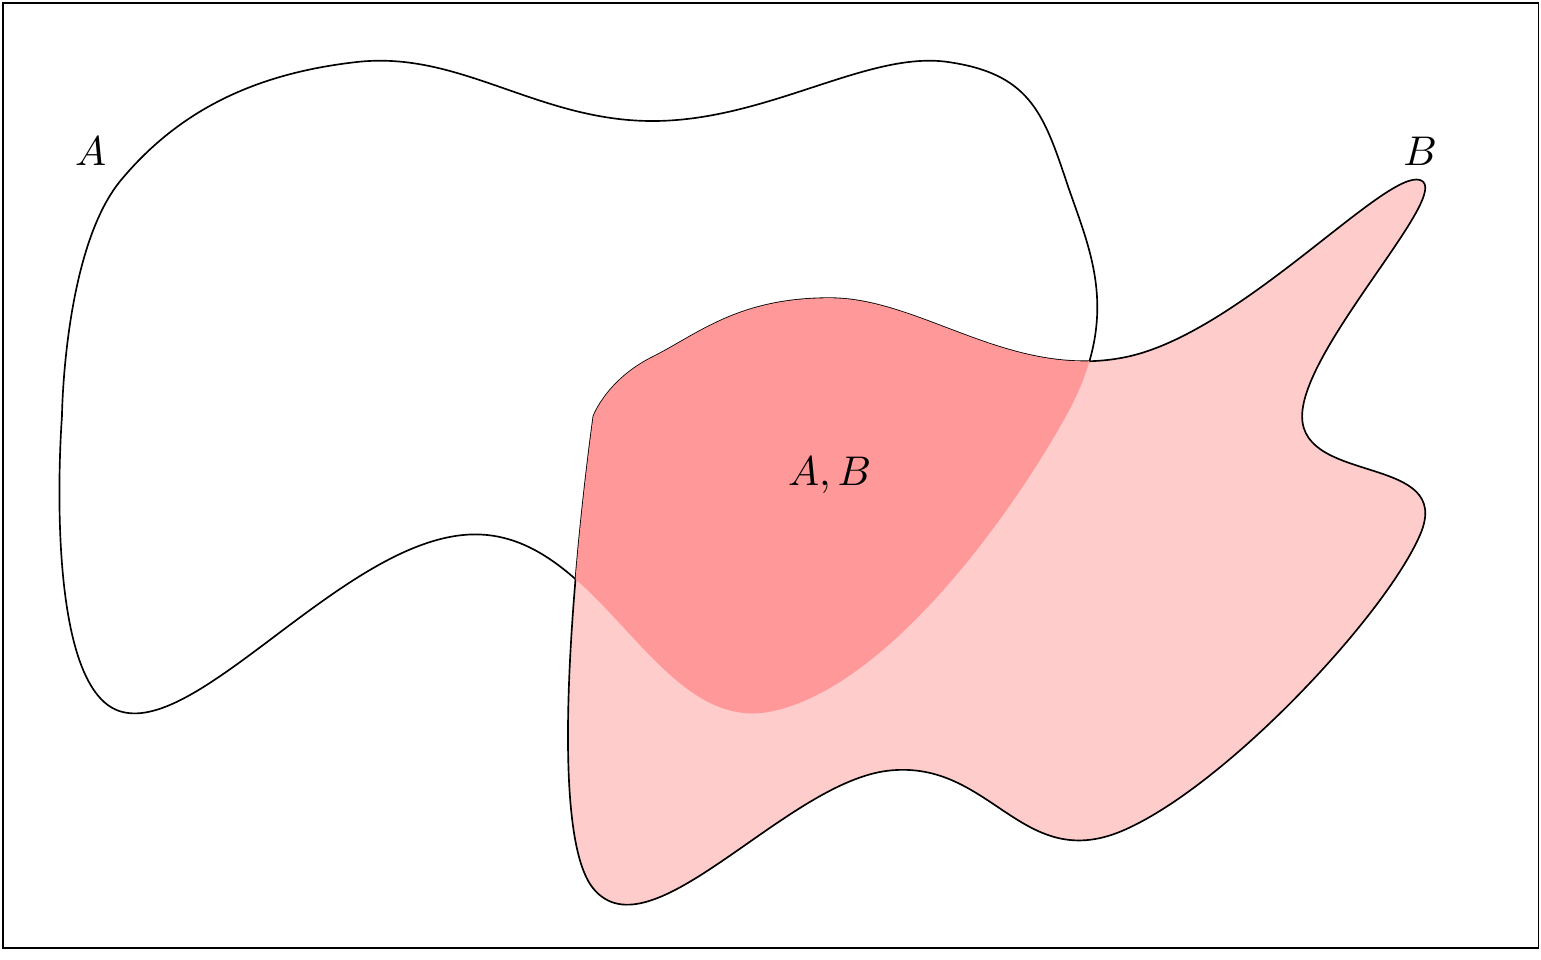
\includegraphics{FerenciTamas_ValszamEsStatAlapvonalai_files/figure-latex/unnamed-chunk-25-1} }\end{center}

Némi játszadozás után levonhatjuk a legfontosabb tanulságot: minél nagyobb a mintaméret, annál kisebb a mintavételi ingadozás mértéke! Azaz, annál kisebb lesz a bizonytalansága a mintából becsült értéknek. Ez egy nagyon fontos megállapítás, hiszen

\begin{itemize}
\tightlist
\item
  azt eddig is láttuk, hogy a mintavételi ingadozás soha nem szüntethető meg (biztos állítást soha nem tudunk tenni), de most már látjuk, hogy mi az az egyetlen dolog, amit viszont tehetünk ellene: megnövelhetjük a mintanagyságot,
\item
  ha ráadásul számszerűsíteni is tudjuk a mintanagyság és a mintavételi ingadozás közti összefüggést (és elárulhatom: tudjuk), akkor meg tudunk oldani olyan problémát, hogy ha megadják milyen biztos becslés kell, akkor meghatározzuk, hogy ahhoz mekkora mintaméret szükséges.
\end{itemize}

Ezekkel a kérdésekkel azonban már kezdünk a következő fejezetünk témájára átkerülni: hogy a becslésben lévő bizonytalanságot hogyan lehet megragadni, jellemezni.

\hypertarget{a-bizonytalansuxe1g-jellemzuxe9se}{%
\chapter{A bizonytalanság jellemzése}\label{a-bizonytalansuxe1g-jellemzuxe9se}}

Az előző fejezetben alaposan körüljártuk azt a megállapítást, hogy a következtető statisztikában nincs biztos válasz. Elkerülhetetlen módon minden válaszunkat bizonytalanság fogja terhelni. A következtető statisztika egyik legnagyobb ereje, hogy e bizonytalanság mértékét \emph{magát} is képes lesz jellemezni -- ebben a fejezetben ezzel a kérdéssel fogunk foglalkozni.

\hypertarget{intervallumbecsluxe9s}{%
\section{Intervallumbecslés}\label{intervallumbecsluxe9s}}

TODO

\hypertarget{hipotuxe9zisvizsguxe1lat}{%
\section{Hipotézisvizsgálat}\label{hipotuxe9zisvizsguxe1lat}}

TODO

\hypertarget{egy-alapvetux151-kutatuxe1smuxf3dszertani-kuxe9rduxe9s}{%
\chapter{Egy alapvető kutatásmódszertani kérdés}\label{egy-alapvetux151-kutatuxe1smuxf3dszertani-kuxe9rduxe9s}}

\epigraph{Statisztikával hazudni könnyű, de statisztika nélkül még könnyebb.}{\textit{Charles Frederick Mosteller}}

A statisztika tulajdonképpen az előző fejezettel befejeződött. Nem tudom megállni azonban, hogy ne hívjam fel a figyelmet pár általános, mondjuk úgy: kutatásmódszertani kérdésre. Azért nem, mert ezek borzasztó gyakran épp a \enquote{statisztikát alkalmazunk!} felkiáltás ürügyén sikkandnak el. Soha nem szabad ugyanis egy dolgot elfelejteni: mindaz a statisztikai apparátus, amiről az elmúlt fejezetekben szó volt \emph{csak és kizárólag} a mintavételi ingadozásból fakadó bizonytalanság kezelésére alkalmas, és a \emph{világon semmit} nem mond egy kutatás összes többi hibaforrásáról! Ezért nagyon rossz, amikor valaki a következtető statisztika alkalmazásával kapott eredményeket, mondjuk a \(p\)-értékeket úgy kezeli, hogy akkor ezzel a kutatás hibáinak problémája le van tudva. A \(p\)-értékek nem egy kutatás hibázásának univerzális metrikái -- simán előfordulhat, hogy egy kutatási domináns hibaforrását \emph{nem} a mintavételi ingadozás jelenti! Éppen ezért fontos, hogy ismerjük ezek közül minimum a legfontosabb problémát, a confounding-ot, mely szinte minden társadalmi-gazdasági (és sok orvosi) vizsgálatban felmerül. Amíg ezt nem tisztáztuk egy vizsgálat kapcsán, addig tizedrangú kérdés, hogy a kapott eredmény a szó statisztikai értelmében szignifikáns-e.

A most következő leírásom orvosi példákat fog hozni\footnote{Ez a fejezet az Interpress Magazinban (IPM) megjelent \href{http://www.interpressmagazin.hu/cikkek/56732-az_orvoslas_tevedesei_1__resz}{cikksorozatom} első néhány részének rövidített, szerkesztett változata.}, de reményeim szerint közvetlenül látszódni fog, hogy ugyanez a kérdéskör hogyan jelenik meg más területeken is.

\hypertarget{az-orvosi-megismeruxe9s-alapkuxe9rduxe9sei}{%
\section{Az orvosi megismerés alapkérdései}\label{az-orvosi-megismeruxe9s-alapkuxe9rduxe9sei}}

Egy friss újsághír szerint egy svéd egyetem kutatói félmillió gyermek környezetét vizsgálták meg, és azt találták, hogy ahol magasabb a légszennyezettség, ott több a mentálisan beteg gyermek. A légszennyezés tehát mentális betegséget okoz! Vagy mégsem\ldots?

Az orvostudomány egy jelentős része ilyen, és ehhez hasonló kérdésekre igyekszik választ adni: okoz-e mentális betegséget a légszennyezés? A mobiltelefon-használat agyrákot? A vöröshús-fogyasztás vastagbélrákot? A császármetszéssel születés megnöveli-e annak kockázatát, hogy a gyermeknek később 1-es típusú cukorbetegsége lesz? És ha az anya paracetamolt szed a terhesség alatt, attól lehet a gyermek autista? Itt van ez az új vérnyomás-csökkentő gyógyszerjelölt, vajon csökkenti-e tényleg a vérnyomást? És okozhat-e alvászavart mellékhatásként?

E kérdésekre számos módszerrel kereshetjük a választ. Alapul vehetünk biológiai (élettani, kórélettani) megfontolásokat, kereshetünk állatmodelleket, amik lehetővé teszik a jelenségek vizsgálatát, tekinthetünk analóg példákat más területről, gyárthatunk matematikai modellt, azonban a jelen cikksorozat tárgya egy más jellegű, ám egyre fontosabb módszer: az empirikus vizsgálat. Az empirikus annyit tesz: \enquote{tapasztalati}, úgyhogy rögtön pontosítanom kell: a legrosszabb orvosi megismerési módszerek is tapasztalatokon alapulnak, ezért talán jobb, ha úgy mondjuk: szisztematikus empirikus vizsgálat. Empirikus, mert az alapján próbáljuk megválaszolni a kérdést, hogy begyűjtünk tényadatokat gyermekek környezetének légszennyezettségéről és a tényleges megbetegedéseikről, és szisztematikus, mert ezt nem ötletszerűen, hanem valamilyen terv szerint tesszük. A kérdés tehát adott: miután megvannak ezek az adatok, hogyan következtethetünk azokból arra, hogy okoz-e mentális betegséget a légszennyezés?

Első ránézésre könnyű dolgunk van: empirikusan dolgozunk ugyebár, ezért begyűjtünk tényadatokat gyermekek lakóhelyének légszennyezettségéről, és esetleges későbbi megbetegedéseikről. Szisztematikusan dolgozunk, ezért a mintavételt alkalmas terv szerint végezzük, például a népességnyilvántartó adataiból teljesen véletlenszerűen választunk ki kellően sok gyermeket. (Tehát véletlenül sem internetes kérdőívet küldünk ki, többek között a \enquote{Megbetegítették a gyermekemet a légszennyezettséggel!!!} Facebook-csoport tagjainak, megkérve, hogy idézzenek fel az összefüggést megerősítő illetve cáfoló példákat.)

A kapott eredmények, a példa kedvéért: a 100 ezer nem légszennyezett helyen élő gyermek közül 1310-nél lépett fel mentális betegség, a 100 ezer légszennyezett környezetben felnövő közül azonban 3750-ben. A különbség drámai. Márpedig szisztematikusan dolgoztunk, a lehető legjobban: véletlenszerűen választott adatokkal, empirikusan vizsgáltuk a kérdést, ráadásul igen nagy mintán, úgyhogy hátradőlhetünk és nagy nyugalommal mondhatjuk: a légszennyezettség mentális betegséget okoz!

Vagy mégsem?

\hypertarget{az-okozatisuxe1g-nyomuxe1ban}{%
\section{Az okozatiság nyomában}\label{az-okozatisuxe1g-nyomuxe1ban}}

A válaszhoz induljunk egy picit távolabbról. Érdemes felidézni az előző alfejezetből, hogy milyen szerteágazóak azok a -- fentihez hasonló -- kérdések, melyekre választ szeretnénk adni az orvostudományban: Okoz-e agyrákot a mobiltelefon használata? A vörös hús fogyasztása vastagbélrákot? A császármetszéssel születés megnöveli-e annak kockázatát, hogy a gyermeknek később 1-es típusú cukorbetegsége lesz? És lehet-e a gyermek autista attól, hogy az anya paracetamolt szed a terhesség alatt? Itt van ez az új vérnyomáscsökkentő gyógyszerjelölt, vajon tényleg csökkenti-e a vérnyomást? Okozhat-e alvászavart mellékhatásként?

Ebben a listában igyekeztem, teljesen szándékosan, a lehető legkülönbözőbb kérdéseket összegyűjteni, melyekben látszólag egyetlen közös pont sincs. Ezt azért tettem, hogy még meglepőbb legyen a következő kijelentésem: azt állítom ugyanis, hogy bármennyire is különbözőnek tűnnek, valójában kivétel nélkül az összes felsorolt kérdés mögött -- és milliónyi egyéb orvosi, egészségügyi kérdés mögött -- pontosan ugyanaz a séma van! Persze, a konkrét részletek nagyon eltérnek, de ha ezektől megtisztítjuk az egyes kérdéseket, akkor a mélyben minden esetben ugyanazt találjuk.

Az egyik komponens: minden kérdésben található valami, amit teljesen általános szóval \emph{expozíciónak} fogunk hívni. Ez szó szerint \enquote{kitettséget} jelent, és tényleg azt is értjük alatta, hogy az alany ki volt téve valamilyen hatásnak. Ezt a legáltalánosabban értjük: a hatás lehet valami, amit szándékosan alkalmazunk az alanyon (pl. gyógyszert adunk neki), lehet valami, amit maga választ (pl. vörös húst fogyaszt), és olyasvalami is, aminek akaratán kívül van kitéve (pl. császármetszéssel született). Érdemes végignézni az összes előbbi példát, csakugyan mindegyikben azonosítható az expozíció, a mobiltelefon-használattól egészen a gyógyszerszedésig.

A másik komponens: minden kérdésben található valamiféle eredmény, kimenet -- ezt fogjuk \emph{végpontnak} hívni. Ez lesz az orvosilag lényeges, általunk vizsgált történés; ismét csak, érdemes egy pillanatra visszanézni az előbbi listára, és mindegyik elemnél megkeresni ezt, az agyráktól az alvászavarig.

Ezzel megvan a séma két \enquote{oldala}, expozíció egyfelől, végpont másfelől, már csak egyetlen komponens hiányzik, amit vizsgálni akarunk minden ilyen és ezekhez hasonló kérdésben: az, hogy az expozíció és a végpont között van-e ok-okozati összefüggés. Szép szóval ezt hívhatjuk kauzalitásnak. Bármennyire is különbözőnek tűnnek a kérdések, e séma mindegyikre illeszkedik, mindegyikben azonosítható az expozíció, azonosítható a végpont, és mindegyikre igaz, hogy okozatiságot kutatunk.

De mit is jelent ez a fogalom? Kézenfekvő értelmezés, hogy megnézzük, hogy hány beteg volt a légszennyezéses csoportban, megnézzük, hogy hány lett \emph{volna} köztük, ha minden más változatlan lett volna, \emph{de} nem lett volna légszennyezés -- és a kettő különbség a légszennyezés hatása. Sajnos ezt a másodikat soha nem ismerhetjük, hiszen ez egy valójában létre nem jött, képzeletbeli helyzet. Éppen ezért jobb híján a nem légszennyezéses csoporthoz viszonyítunk, tehát nem \emph{ugyanazon} csoport tényleges és képzeletbeli helyzetét vizsgáljuk, hanem két \emph{különböző} csoport tényleges helyzetét viszonyítjuk \emph{egymáshoz}. Lényegében azt mondjuk, hogy a nem légszennyezett környezetben felnövő gyermekek adatai mutatják, hogy mi lett \emph{volna}, ha a légszennyezett környezetben felnövőknél nem lett volna légszennyezés.

Csakhogy ez egy nagyon erős feltevés: kizárólag akkor igaz, ha a két csoport semmi másban nem tér el, egyedül a légszennyezettség tényében.

A tételmondatot mindenesetre megfogalmazhatjuk: Az expozíció akkor van okozati összefüggésben a végponttal, ha a csak az expozícióban eltérő csoportok eltérnek a végpontban, mégpedig olyan mértékben, ami már nem tudható be a véletlen ingadozásnak. Ez utóbbi az, amit már tudunk kezelni a következtető statisztika apparátusával! Csakhogy a mondat első felében is komoly csapdák vannak elrejtve\ldots{}

\hypertarget{a-confounding-probluxe9muxe1ja}{%
\section{A confounding problémája}\label{a-confounding-probluxe9muxe1ja}}

Ebben a tételmondatban tehát van egyetlen egy szó, ami iszonyatos bonyodalmakat okoz: az, hogy \enquote{csak}. Biztos, hogy az összehasonlított csoportjaink kizárólag csak az összehasonlítás tárgyában, tehát az expozícióban térnek el? Biztos, hogy a légszennyezett területen felnövő és az egészséges levegőben felnövő gyermekek között \emph{csak és kizárólag} az a különbség, hogy milyen a levegőminőség a lakhelyükön\ldots?

Dehogy! A nagyobb légszennyezettségű területek nagyon gyakran épp a városok peremkerületeit jelentik, az ipari negyedeket, az elavult fűtésű, leszakadt részeket. Itt azonban tendenciájában inkább rossz körülmények között élő, kevésbé tehetős családba született (egyszóval: rosszabb szocioökonómiai helyzetű) gyermekek fognak lakni. Igen ám, de a rosszabb szocioökonomiai helyzet egy sor betegség magasabb kockázatát hordozza --- mi van, ha a mentális betegségek is ezek közé tartoznak? Mert a rosszabb szocioökonómiai szegmensben a várandósok kevésbé férnek hozzá a szülés előtti gondozáshoz, közülük több dohányzik vagy fogyaszt alkoholt a várandósság alatt. A gyermekekre sem csak a rosszabb levegő hat, hanem a rosszabb táplálkozás, hogy kevésbé vesznek részt szűréseken és így tovább, és így tovább.

Innentől kezdve, ha találunk is különbséget a mentális megbetegedések előfordulásában a két csoport között, \emph{nem tudhatjuk}, hogy az minek a következménye: az általunk vizsgált levegőminőségbeli eltérésnek, az ezzel -- \emph{óhatatlanul!} -- \emph{együttjáró} egyéb eltéréseknek, vagy esetleg ezek keverékének?! Ezt nem tudhatjuk -- hiszen az összehasonlított csoportok nem \emph{csak} az összehasonlítás szempontjában tértek el.

A problémát tehát az jelenti, hogy a két változó kapcsolatát \emph{megzavarja} egy harmadik változó, mely egyszerre hat az expozícióra \emph{és} a végpontra. Ez a naiv elképzelés:

\begin{center}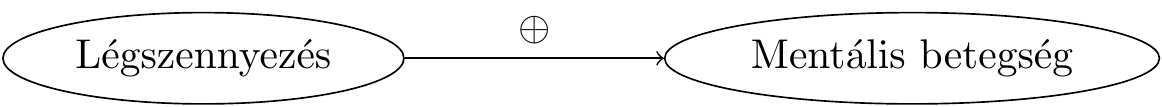
\includegraphics{FerenciTamas_ValszamEsStatAlapvonalai_files/figure-latex/unnamed-chunk-27-1} \end{center}

És ez a valódi helyzet:

\begin{center}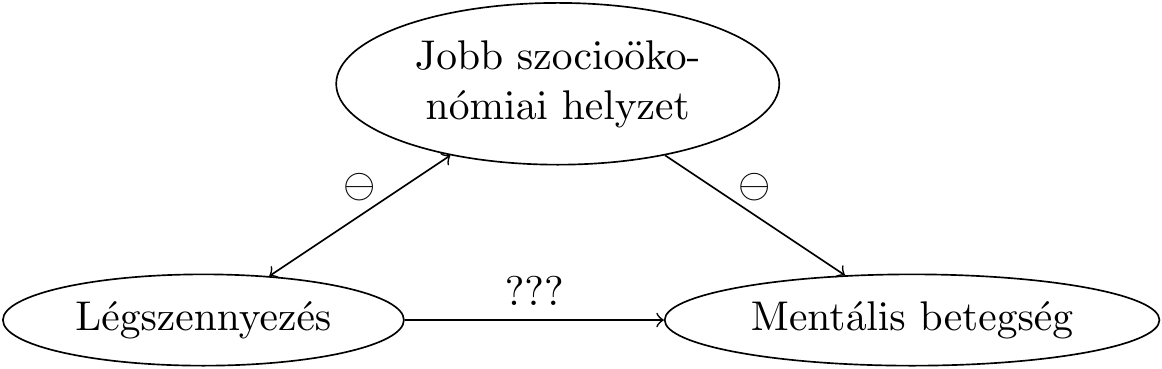
\includegraphics{FerenciTamas_ValszamEsStatAlapvonalai_files/figure-latex/unnamed-chunk-28-1} \end{center}

Ennek következtében elképzelhető, hogy a légszennyezettségnek valójában \emph{nincs is a világon semmilyen} hatása a mentális betegségekre, amit látunk, az egy \emph{látszólagos} hatás, annak következtében, hogy a légszennyezett területen felnövő gyermekek körében egész egyszerűen több a rossz szocioökonomiai helyzetű, ami pedig a \emph{valódi} oka a több mentális betegségnek!

Ha valaki nem hiszi el, hogy ilyen létezhet, akkor nézze meg képzeletbeli adatgyűjtésünk részletesebb eredményeit, melyet a következő táblázat mutat:

\begin{longtable}[]{@{}llll@{}}
\toprule
& Légszennyezett & Nem légszennyezett & Összesen\tabularnewline
\midrule
\endhead
Rossz szocioökonómiai helyzet & 6\% (3300/55000) & 6\% (375/6250) & 6\% (3675/61250)\tabularnewline
Jó szocioökonómiai helyzet & 1\% (450/45000) & 1\% (935/93750) & 1\% (1385/138750)\tabularnewline
Összesen & 3,8\% (3750/100000) & 1,3\% (1310/100000) & 2,5\% (5060/200000)\tabularnewline
\bottomrule
\end{longtable}

Ebben a táblázatban valami első ránézésre egészen paradox dolog látható. (Azért írtam oda nem csak a százalékokat, de a számokat is, mert néhányan azt szokták mondani, hogy ez matematikailag is lehetetlen. Erről szó nincs, ha valaki nem hiszi, adja össze és ossza el a feltüntetett számokat!) Mert mit látunk? Azt, hogy a rossz szocioökonómiai helyzetű gyermekek körében \emph{nincs} hatása a légszennyezésnek (így is, úgy is 6\% az előfordulása), a jó szocioökonómiai helyzetű gyermekek körében \emph{szintén nincs} hatása (1\% így is, úgy is) -- összességében viszont \emph{mégis} van! Hiszen az 1,3\% megnőtt 3,8\%-ra, ahogy azt a felvezetőben is írt számok mutatják. Ez meg hogy a csudában lehet? -- kérdezhetné valaki. Se egyik csoportban nincs hatása, se a másikban, de összességében mégis van?!

Rakjuk most össze, hogy mi is történt itt. A problémát az okozta, hogy volt egy változónk, mely \emph{egyszerre} tudott két dolgot: \emph{egyrészt} összefüggött az expozícióval (nézzük meg, a jó szocioökonómiai helyzetűeknek csak harmada élt légszennyezett területen, a rosszaknak majdnem 90\%-a), \emph{másrészt} befolyásolta a végpontot a légszennyezettségtől \emph{függetlenül}, \emph{önmagában} is (az 1\%-os előfordulást 6\%-ra emelte). Az ilyen változókat szokás zavaró változónak, vagy -- magyarul is gyakrabban használt angol kifejezéssel -- confoundernek nevezni; a jelenségnek magának pedig \textbf{confounding} a neve. (Ez egy nagyon találó angol kifejezés, amire sajnos nem honosodott meg hasonlóan frappáns magyar elnevezés. A \enquote{confounding} ugyanis szó szerint azt jelenti, hogy \enquote{egybemosódás}: a probléma valóban az, hogy az általunk vizsgált eltérés \emph{egybe van mosódva} egy vagy több egyéb eltéréssel.)

Ez az oka annak, hogy a naiv módszer (\enquote{több-e a mentálisan beteg a magasabb légszennyezettségű területeken?}) csábító mivolta ellenére is \emph{teljesen fals}! Hiába is dolgoztunk empirikusan, és hiába is gyűjtöttünk szisztematikusan adatokat.

Fontos felhívni rá a figyelmet, hogy a \enquote{teljesen fals} természetesen nem azt jelenti, hogy az eredményünk akkor valójában azt jelenti, hogy nem okoz mentális betegséget a légszennyezettség -- természetesen okozhat, csak ez \emph{nem következik} abból, hogy több a mentálisan beteg a szennyezettebb levegőjű területeken! \emph{Önmagában} ez az együttjárás \emph{nagyon kevéssé bizonyítja} az okozati összefüggést. Azt mondhatjuk, hogy nagyobb légszennyezettség \emph{együtt jár} a több mentális betegséggel, de hogy a nagyobb légszennyezettség \emph{okoz-e} több mentális betegséget, az egy sokkal-sokkal fogósabb kérdés, aminek kapcsán, mint a fentiek is mutatják, roppant óvatosan kell eljárni.

Ez az ilyen jellegű adatok értékelésének egyik legnagyobb problémája (mely a laikus sajtóban is lépten-nyomon visszaköszön). A valóságban ráadásul messze nem olyan egyszerű a helyzet, mint a fenti táblázatban, ahol van egy szem confounderünk. A valós helyzetek általában ennél sokkal-sokkal kuszábbak.

Ennek illusztrálására vegyünk egy másik példát a cikk elejének listájáról: a császármetszéssel születés megnöveli-e az 1-es típusú cukorbetegség kockázatát? A császármetszéssel születők között több az 1-es típusú cukorbeteg, de -- most már tudjuk -- ez nem sokat jelent, hiszen mi van, ha vannak egyéb eltérések is a csoportok között? Ez csakugyan így van: a következő ábra mutatja, immár egy valós orvosi példán, a legfontosabb confoundereket ebben az esetben. Még itt se mondhatjuk persze, hogy ez az összes, de ez már valóságközelibb.

\begin{center}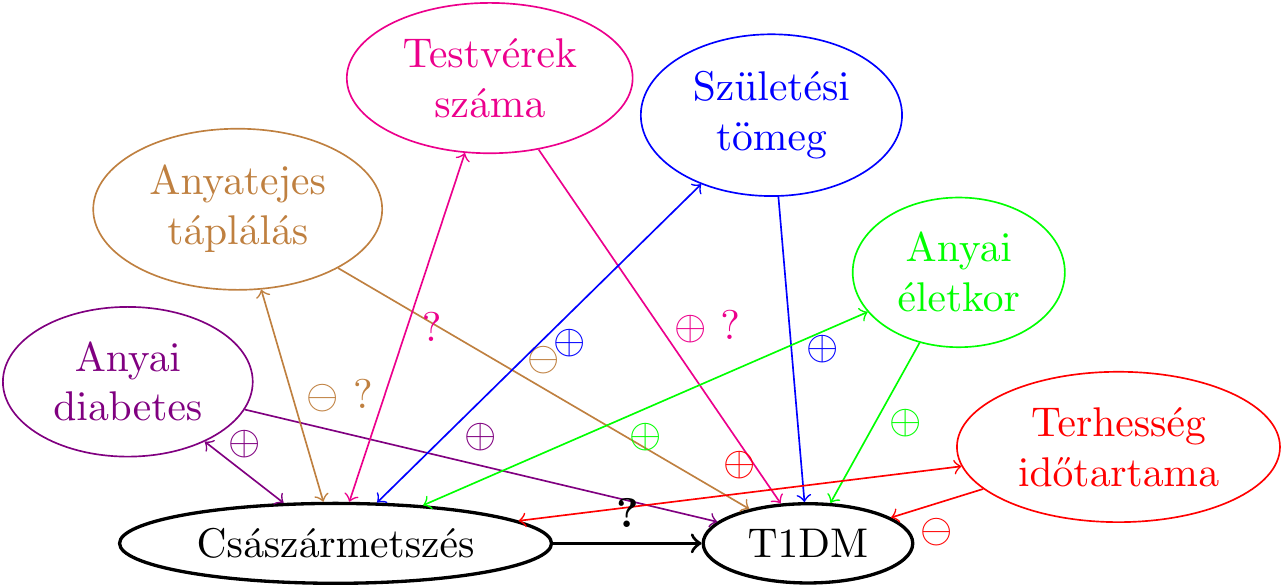
\includegraphics{FerenciTamas_ValszamEsStatAlapvonalai_files/figure-latex/unnamed-chunk-29-1} \end{center}

Példának okáért, az anyai diabetes és a császármetszés közötti nyílon pozitív jel van, mert a cukorbeteg anyáknak általában nagyobbak a magzataik, és ez a különféle téraránytalanságok miatt gyakrabban vezet császármetszéshez. Másrészt a cukorbetegségnek van egy erős genetikai komponense, így az anyai cukorbetegségből a gyermekéhez is pozitív nyíl vezet. És már ennyi is elég, hogy bajban legyünk: innentől kezdve, még ha azt is találjuk, hogy a császármetszéssel születettek körében több lesz később cukorbeteg (egyébként tényleg ez a helyzet), akkor sem tudhatjuk, hogy mi a valódi ok: csakugyan a császármetszés, vagy egyszerűen csak az, hogy a császármetszéssel születőknek gyakrabban cukorbeteg az édesanyja? És ez még csak az első confounder volt!

Érdemes megnézni a másodikat, az anyatejes táplálást is. Ez rámutat arra, hogy az expozíció és a confounder között nem érdekes, hogy milyen az okozati kapcsolat iránya (az eddigi példákkal szemben itt most aligha arról van szó, hogy az anyatejes táplálás befolyásolja, hogy korábban császármetszés történt-e\ldots), csak az fontos, hogy kapcsolat van. És csakugyan, a császármetszéssel szülő nők ritkábban táplálják anyatejjel a gyermeküket, ez így van a valóságban, és most az mindegy is, hogy ennek mi az oka. Másrészt az anyatejes táplálás (számos egyéb előnye mellett) csökkenti a cukorbetegség kockázatát is -- és akkor e ponton megint meg vagyunk lőve\ldots{} és még közel nem vagyunk a sor végén.

\hypertarget{zavaruxf3-vuxe1ltozuxf3ktuxf3l-a-megzavart-olvasuxf3kig}{%
\section{Zavaró változóktól a megzavart olvasókig}\label{zavaruxf3-vuxe1ltozuxf3ktuxf3l-a-megzavart-olvasuxf3kig}}

Nem véletlenül írtam korábban, hogy a naiv módszer nagyon \enquote{csábító} tud lenni. Képzeljük csak el, pláne némi marketinggel meghintve: látványos grafikon, rajta a nem légszennyezett területen felnövők körében a kockázat (kicsi oszlop), mellett a légszennyezett területek adata (oszlop kiüti az oldal tetejét), szomorú anyuka megrázó beszámolója mentálisan beteg gyermekéről, természetesen hangsúlyozva a levegőminőséget stb. stb. Vajon 100 emberből hánnyal hitetné el a légszennyezettség szerepét\ldots? (És hányan mondanák azt, hogy \enquote{hohó, de hát itt óvatosnak kell lenni, mert a szocioökonómiai státuszon keresztül megvalósuló confounding van!}\ldots?)
Ha jobban megnézzük, mindennapi egészségügyi megállapításainkat lépten-nyomon átszövi ez a probléma. Nézzük meg kedvenc internetes portálunk egészségügyi rovatát is\ldots{}

\enquote{A több zöldséget fogyasztók 10 évvel tovább élnek!} Biztos, hogy a több zöldséget fogyasztók csak a zöldségfogyasztás mértékében térnek el a kevesebb zöldséget fogyasztóktól? Fogadjuk el, hogy igaz az állítás, és tényleg együtt jár a több zöldségfogyasztás a hosszabb élettartammal. Akkor végül is igaz ez a mondat, minek rajta kötözködni? -- kérdezhetné valaki. Szó nincs erről, ez nem akadékoskodás, éppen ellenkezőleg, ez a legfontosabb kérdés. A mondat nyilván azt akarja sugallani, hogy együnk több zöldséget, hogy tovább éljünk. De ha valójában az előző nem okozati kapcsolat, csak együttjárás, akkor -- mivel a valódi ok más volt -- ezzel \emph{nem megyünk semmire}! Márpedig számunkra ez a fontos: ha egy ilyen cikket olvasva életünket úgy változtatjuk meg, hogy növeljük a zöldségfogyasztásunkat, akkor \emph{várhatjuk-e ettől}, hogy megnő az élettartamunk?

A sor ugyanerre a mintára sajnos igen hosszan folytatható. \enquote{Az indiai konyha rengeteg curry-t használ, és lám, velünk szemben ott szinte ismeretlenek a gyulladásos bélbetegségek!} (Biztos, hogy India és Magyarország között csak és kizárólag az az egyetlen különbség, hogy a főzéshez más mennyiségű curry-t használunk?) \enquote{Azokban az amerikai államokban, ahol többet alszanak, kevesebb a depressziós!} (Biztos, hogy ezen amerikai államok csak és kizárólag az alvással töltött órák számában térnek el a többitől?) A legszebb, amikor ugyanazt eljátsszuk oda és vissza is: \enquote{30 éve még nem használták ilyen széles körben a vérnyomás-csökkentőket, és jóval több is volt a magas vérnyomásos beteg!} (Biztos, hogy 2018 és 1988 között az egyetlen különbség a vérnyomás-csökkentők használatának a mértéke?) \enquote{30 éve még nem használták ilyen széles körben a védőoltásokat, és jóval kevesebb is volt az autista!} (Biztos, hogy 2018 és 1988 között az egyetlen különbség a védőoltások használatának a mértéke?)

\hypertarget{egy-aranyuxe9rmes-megolduxe1s}{%
\section{Egy aranyérmes megoldás}\label{egy-aranyuxe9rmes-megolduxe1s}}

Mit tudunk tenni a confounding problémája ellen? \emph{Törekedni} sokféleképp lehet arra, hogy a csoportok csak a vizsgált tényezőben térjenek el, de \emph{biztosan} elérni csak egyféleképp. Tulajdonképpen az a meglepő, hogy a megoldás milyen későn merült fel. 1931-ben a michigan-i William H. Maybury Tüdőszanatórium orvosa, James Burns Amberson ki akarta deríteni, mégpedig empirikusan, hogy egy sanocrysin nevű szervetlen aranyvegyület vajon gyógyítja-e a TBC-t (elég sok írás született ennek lehetőségéről akkoriban). Az -- \emph{ugyebár!} -- nem jó megoldás, hogy összehasonlítjuk a gyógyszert kapó és gyógyszert nem kapó betegek gyógyulását, hiszen mi van, ha ők másban is eltérnek a gyógyszerben részesülés tényén túl? Mi van, ha a gyógyszert inkább kapták a fiatalok (vagy pont, hogy az idősek), inkább kapták a férfiak vagy a nők, inkább kapták a több vagy kevesebb társbetegséggel rendelkezők stb. Ez jelen esetben a legkevésbé sem elméleti spekuláció, nagyon is könnyen lehet, hogy egy új, még nem jól ismert kezelést inkább a jobb állapotú és így egyúttal legjobb gyógyhajlamú betegeknek írnak fel inkább az orvosok. Tehát a gyógyszert kapó és nem kapó csoportok ilyen összehasonlítása teljesen félrevezető lehet -- belefutottunk a confounding problémájába.

Amberson és munkatársai egy huszárvágással megoldották a problémát: pénzfeldobással döntötték el, hogy ki kapjon sanocrysin-t! És ezt most nem irodalmi fordulatként mondom, hanem a szó szoros értelmében: Amberson \emph{konkrétan} feldobott egy pénzérmét és az alapján adott sanocrysin-t vagy egyszerű desztillált vizet a betegeknek, hogy fejet vagy írást kapott, ezt pontosan dokumentálta is a cikkében. Még arról is gondoskodott, hogy a két szer külsőleg ne legyen megkülönböztethető, és, hogy a dobás eredményéről ne tudjon a beteg, csak két orvos és a beadó nővér.

És ennyi. Ezzel, a történelemben először, megoldódott a confounding problémája. Majd látni fogjuk, hogy az ismert confounderek kiszűrésére lesz módunk: ha eszünkbe jut, hogy a gyógyszert inkább fiatalabbak, vagy inkább férfiak kapják, és ezért feljegyezzük nem csak gyógyszerben részesülés tényét, hanem azt is, hogy az alany milyen idős és mi a neme, akkor ezeket -- mint zavaró tényezőket -- ki fogjuk tudni szűrni. De ennek minimális feltétele, hogy eszünkbe jusson, hogy mik a confounderek, \emph{és} le is tudjuk őket mérni (egy olyannál, mint a \enquote{szocioökonómiai státusz} ez utóbbi sem nyilvánvaló). Amberson megoldásában, amit az orvosi irodalomban \emph{randomizációnak} szokás nevezni, az a zseniális, hogy \emph{minden} confoundert kiszűr, azokat is, amiket nem tudunk feljegyezni, sőt, azokat is, amik eszünkbe sem jutnak! Tegyük fel például, hogy kiderül, hogy a kékszeműeknek az orvosok inkább adnak sanocrysin-t \emph{és} a kék szem egyúttal növeli a TBC-ből való gyógyhajlamot. Ez csúnyán tönkretenné az összes vizsgálatot, hiszen ki gondolna arra, hogy a szemszínt is fel kell jegyezni, de vegyük észre, hogy -- mert ez a lényeg -- Amberson módszere \emph{még ekkor is működik}! Hiszen a pénzfeldobás révén a kékszeműek arányában \emph{sem} lesz szisztematikus különbség a két csoport között! Ugyanúgy, mint ahogy nem lesz szisztematikus különbség a nemi összetételben, az életkori összetételben, és egyáltalán: \emph{semmilyen} szempontban sem! Úgy is mondhatjuk, hogy a randomizáció kiszűri, ráadásul \emph{automatikusan} kiszűri mind a végtelen számú potenciális confoundert -- azokat is, amiket nem tudtunk feljegyezni, sőt, azokat is, amikről \emph{eszünkbe sem jut}, hogy confounderek! Ez a randomizált kutatások hihetetlen nagy előnye.

(Ez a kiszűrés természetesen nem azt jelenti, hogy biztosan minden szempont tökéletesen kiegyensúlyozott lesz a csoportok között. A pénzfeldobás szeszélye folytán \emph{előfordulhat}, hogy puszta véletlenségből több kékszemű lesz az egyik csoportban, de be lehet látni, hogy mivel ez csak a véletlen szeszélye folytán állt elő, így nem befolyásolja a fenti állításokat.)

\hypertarget{megfigyeluxe9s-uxe9s-kuxedsuxe9rlet}{%
\section{Megfigyelés és kísérlet}\label{megfigyeluxe9s-uxe9s-kuxedsuxe9rlet}}

Amberson módszerének egy roppant fontos jellemzője van: befolyásolnunk kell hozzá, hogy ki kap gyógyszert (expozíciót). Azokat az orvosi vizsgálatokat, ahol a kutatók aktívan befolyásolják az expozíciót, \textbf{kísérletes vizsgálatnak}, azokat, ahol csak passzívan feljegyzik, hogy mi történt, de nem befolyásolják azt, \textbf{megfigyeléses vizsgálatnak} szokás nevezni.

A kísérletek története messzire nyúlik vissza, ám a korai kísérletek problémája az, hogy mindig ott van a lehetőség, hogy az orvos, akár teljesen tudattalanul is, de célirányosan befolyásolja, hogy ki melyik csoportba kerül. Ezt már a XIX. század végére felismerték, ezért akkorra divatba jöttek az úgynevezett \enquote{váltakozó besorolású} kutatások, ami azt jelentette, hogy minden második beteg kapta meg a vizsgált gyógyszert, minden második nem. Ez már egészen közel van a randomizált vizsgálatokhoz (az csak nem befolyásolja a gyógyulásomat, hogy páratlan sorszámú beteg voltam-e aznap a kórházban!), de valójában még itt is jelentkezhet az előbbi probléma: sokszor leírták például, hogy az orvosoknak megesett a szíve egy betegen, ezért igyekeztek úgy rendezni az ellátást, hogy a kezelt csoportba kerülhessen. Ez nyilvánvalóan elrontotta a dolgot, ha mondjuk a legrosszabb állapotú betegeknél került erre a leggyakrabban sor. Éppen ezért a váltakozó besorolás helyét a XX. század közepe felé átvette a randomizált besorolás, különösen, hogy a híres statisztikus Ronald Fisher ennek az elméletét is kidolgozta (egyébként már Amberson orvosi alkalmazása előtt).

Látható tehát, hogy a kísérletes vizsgálatok hihetetlenül nagy és roppant fontos előnye, hogy elvileg mentesek tudnak lenni a confoundingtól. (Gyakorlatilag persze nem feltétlenül: kísérletet is lehet rosszul csinálni.) A megfigyeléses vizsgálatoknál viszont, bármennyire is óvatosan járunk el, mindig a fejünk fölött fog Damoklész kardjaként lebegni a confounding: biztos, hogy minden tényező, amiben az összehasonlított csoportok eltérnek -- az összehasonlítás tárgyán kívül -- eszünkbe jutott? Biztos, hogy mindegyiket le tudjuk mérni? Biztos, hogy mindegyiket jól ki tudjuk szűrni?

Mindezeket látva adja magát a kérdés: akkor miért nem csinálunk mindig kísérletet?

Erre a kérdésre vannak nyilvánvaló és kevésbé nyilvánvaló válaszok. A legnyilvánvalóbb, hogy bizonyos helyzetekben egyszerűen lehetetlen: valószínűleg apróbb nehézségeink támadnának a kutatásetikai bizottság előtt egy olyan kutatási tervvel, amelyben szülőnőket randomizáltan akarunk \enquote{császármetszetni} -- függetlenül attól, hogy szükségük van-e rá -- azért, hogy kiderítsük, hogy a császármetszés okoz-e cukorbetegséget (pedig, módszertani szempontból ez lenne a legjobb!). Hasonlóan nehéz embereket randomizáltan légszennyezett és kevésbé légszennyezett területen \enquote{lakatni}, csak hogy visszatérjünk az eredeti példánkra. Ilyen esetekben mindenképp maradnak a megfigyeléses vizsgálatok, azok minden bajával együtt is.

Az érdekes az, hogy néha akkor is csinálunk megfigyeléses vizsgálatot, ha lehetne kísérletet is (vagy akár ténylegesen végeztek is kísérlet). Ez is mutatja, hogy a kísérleteknek más hátrányaik is vannak, túl azon, hogy drágák, idő- és szervezésigényesek.

Az egyik probléma, hogy a kísérletekben, épp az említett szervezésigény miatt, korlátozott a bevonható betegek köre. A néhány ezer fős kísérlet a legtöbb területen már nagynak számít, a néhány tízezer fő pedig már nagyon nagynak, egy ennél is nagyobb kísérletet pedig csak extrém nehezen lehet megszervezni. (Ebből adódóan nagyon kevés ilyenre van példa. Az utóbbi idők legnagyobb orvosi kísérlete, melyben minden egyes alany egyénileg randomizálásra került, a CAPITA kutatás volt, melyben azt vizsgálták, hogy egy pneumococcus elleni oltás tényleg csökkenti-e a pneumococcus okozta tüdőgyulladások előfordulását 65 év felett. Elképesztő számú alanyt, 85 ezer főt vontak be, ehhez két év és 101 központ kellett, megszámlálhatatlan közreműködővel; sejthetőleg százmillió dolláros nagyságrendbe került ez az egyetlen kísérlet.) Hogy ez miért fontos? Azért, mert a nem elegendően nagy mintanagyság korlátozza, hogy milyen nagyságú hatást tudunk észrevenni, legyen szó akár kívánt hatásról, akár mellékhatásról, ha például egy gyógyszerről beszélünk. Ha kicsi a mintanagyság, akkor egy kis javulást, vagy egy ritkán jelentkező mellékhatást nincs sok esélyünk észrevenni. Pontosan az előbbi a magyarázat a CAPITA esetére is: a pneumococcus okozta tüdőgyulladás nem fordul elő sűrűn, így az oltás, legyen bármilyen hatásos is, \enquote{darabra} csak kevéssel tudja csökkenteni a tüdőgyulladások számát. És csakugyan: még a 85 ezer alany is csak arra volt elég, hogy összesen kevesebb, mint 200 -- a vizsgálat szempontjából fontos típusú -- tüdőgyulladás előforduljon. De ugyanez a helyzet a mellékhatások terén is: ha egy mellékhatás csak minden 10 ezredik embert érinti, akkor minden matematikai indoklás nélkül is érezhető, hogy egy 5 ezer fős kutatásban esélyünk sem lesz észrevenni (pedig ez egyáltalán nem kis kísérlet!). Megfigyeléses vizsgálatokkal ezzel szemben összehasonlíthatatlanul könnyebben elérhető ilyen, vagy akár ennél is nagyobb mintanagyság. Gondoljunk arra, hogy a megfigyeléses vizsgálat sok esetben úgy néz ki, hogy adatbázisokból kérdezünk le alanyainkra vonatkozó információkat -- itt a kutatás tehát nem azt jelenti, hogy \emph{fizikailag} alanyokat kell kezelnünk, hanem azt, hogy a számítógép előtt ücsörögve lekérdezéseket kell írogatnunk. A kettő bonyolultságát egy napon nem lehet említeni\ldots! Én magam is -- harmincéves adjunktusként, 2 kutatótársammal -- részt vettem olyan vizsgálatban, melyben néhány hónap alatt, és nulla finanszírozással, 400 ezer magyar beteg adatait dolgoztuk fel -- a CAPITA esetében kutatók és segéderők ezreire és évekre volt szükség, meg mellesleg annyi pénzre, mint a Semmelweis Egyetem éves költségvetése, hogy 85 ezer alanyt össze tudjanak szedni\ldots{}

A másik, előbbihez hasonló gyökerű probléma a kísérletekkel, hogy abban is korlátozottak, hogy mennyi ideig lehetséges az alanyok utánkövetése. A gyakorlatban néhány hónap vagy legfeljebb néhány év érhető el (de az alanyok kihullása a vizsgálatból -- nem megy el a következő vizitre, mert elfelejti, elköltözik, elveszti az érdeklődését stb. -- már ekkor is általában igen nagy probléma). Ennél hosszabb kísérlet lényegében kivitelezhetetlen, vagy csak a legelemibb adatok (például: életben van-e egyáltalán még az alany) gyűjthetőek be. Világos, hogy ez miért gond: amíg a kevés alany azt limitálja, hogy milyen nagyságú hatást tudunk észrevenni, addig a rövid utánkövetés azt korlátozza be, hogy mennyi idő alatt kialakuló hatást -- legyen az akár kívánt hatás, akár mellékhatás -- tudunk észrevenni. Szinte esélytelen, példának okáért, kísérlettel eldönteni, hogy egy gyerekkori táplálkozási szokás vagy orvosi beavatkozás okozhat-e egy tipikusan időskorban, vagy akár felnőttkorban jelentkező betegséget. De itt is elmondható: megfigyeléses vizsgálatokkal nem feltétlenül reménytelen a helyzet, hiszen adatbázisokból sokszor akár több évtizedes átfogású adatok is könnyen kigyűjthetőek.

A harmadik lehetséges probléma a kísérletekkel, hogy a kísérletben részt vevő alanyok -- még a legjóhiszeműbb tervezés esetén is -- szükségképp egy elég speciális, \enquote{steril} populációt jelentenek, már pusztán abból is adódóan, hogy hogyan verbuválják ezeket az alanyokat. Ez mindig felveti azt a kérdést, hogy találjunk bármit is a kísérlet alanyai körében, az vajon mennyire vonatkoztatható az \emph{összes} alanyra\ldots? Megfigyeléses vizsgálatoknál ez a probléma sokkal kevésbé jelentkezik: gyakran akár az összes alany is bevonható a vizsgálatba, így aztán egész biztos nincs probléma az összes alanyra vonatkoztatással.

\hypertarget{a-juxf3-a-rossz-uxe9s-a-kuxf6zepesnuxe9l-nuxe9mileg-gyenguxe9bben-juxf3}{%
\section{A jó, a rossz, és a közepesnél némileg gyengébben jó}\label{a-juxf3-a-rossz-uxe9s-a-kuxf6zepesnuxe9l-nuxe9mileg-gyenguxe9bben-juxf3}}

Összességében véve tehát a legfontosabb megállapítás, hogy nem lehet olyat mondani, hogy a kísérlet és a megfigyelés közül az egyik \enquote{jó}, a másik meg \enquote{rossz}. Mindkettőnek jellemző előnyei és hátrányai vannak, így az, hogy melyik a szerencsés választás, mindig a konkrét kérdéstől függ: van ahol az egyik, van ahol a másik, a kérdés az, hogy az adott problémának mik a jellemzői. Az előbbi pontban mondottakat szem előtt tartva nagy vonalakban már mi is tudunk választani!

A \enquote{nincs jó meg rossz} a fentinél általánosabban is igaz. Minden kutatásnak vannak hibaforrásai. Ilyen a confounding és ilyen a véletlen ingadozás is. Bizonyos kutatásokban több hibaforrás van, vagy komolyabb súlyúak vannak, másokban kevesebb. Van egy szó, amit nagyon szeretek erre: a \emph{bizonyítóerő}. Kifejezi, hogy a tanulmányok -- ilyen értelemben vett -- értéke nem bináris, mint azt néhányan hajlamosak gondolni: nagyon ritkán van olyan, hogy egy kutatás \enquote{tökéletes} (és így ami abban olvasható, az úgy van és pont) vagy, hogy \enquote{teljesen hasznavehetetlen} (ezért bármi is olvasható benne, semmit nem jelent). A valóságban ez egy folytonos skála: arról, hogy a szennyezettebb területeken több mentálisan beteg gyermek él sem mondható, hogy semmit sem jelent (a confounding miatt) -- csak épp borzasztóan alacsony a bizonyítóereje (arra nézve, hogy a légszennyezettség mentális betegséget okoz).

Valójában tehát nincs éles határvonal kísérletes és megfigyeléses bizonyíték között; minden kutatást a saját erényei és korlátai alapján kell értékelni. Ezt legékesebben az bizonyítja, hogy a különböző bizonyítékok \enquote{egy ligában játszanak}, már olyan értelemben, hogy lehet, hogy az általánosságban gyengébbnek tekintett bizonyítékok -- például megfigyeléses vizsgálatok -- képesek lehetnek kiváltani a kísérletes bizonyítékokat. Kipróbálta-e bárki, hogy vakbélgyulladásban a vakbélműtét hatásos beavatkozás a semmittevéshez képest? Meglepődnék\ldots{} Pedig borzasztó egyszerű volna! Csak fogni kellene 200 vakbélgyulladásos beteget, véletlenszerűen 100-at megműteni, és megvárni, amíg 99 gyógyultan hazamegy (nem 100-at mondtam, mert legyen a műtétnek is valamicske kockázata), 100-zal nem csinálni semmit, és megvárni, amíg 99 is az intenzív osztályra kerül perforált vakbéllel (nem 100-at mondtam, mert azért spontán is lehessen meggyógyulni), és voila, meg is van az igen magas bizonyítóerejű bizonyítékunk a vakbélműtét hatásosságára! Egész érthetetlen módon nem tudok róla, hogy ezt bárki megcsinálta volna\ldots{} Vagy mondjuk kipróbálta-e bárki randomizált kísérletben, hogy ha nagy magasságban kiesünk egy repülőgépből, akkor jót tesz-e, ha van nálunk ejtőernyő?

Bocsánat, ez utóbbi kérdésre lehet pontos választ adni: Smith és szerzőtársa 2003-as cikkükben -- a neves orvosi folyóirat, a British Medical Journal karácsonyi különszámában jelent meg -- nagyon alapos irodalomkutatást végeztek a témában. Pontosan definiálták az expozíciót (ejtőernyővel rendelkezés szabadesés esetén) és a végpontot (halál, vagy komoly trauma -- a traumatológiában általánosan használatos ISS sérüléssúlyossági pontszám 15-nél nagyobb -- fellépése a földbecsapódáskor), rendkívül átfogó, több adatbázisra kiterjedő, pontosan dokumentált irodalomkeresést végeztek, majd arra a megdöbbentő eredményre jutottak, hogy elképesztő módon egyetlen egy vizsgálat sem volt, melyben embereket repülőgépből dobáltak volna ki, randomizáltan ellátva őket ejtőernyővel és vizsgálva a végpontot! Azaz, mondják a szerzők -- nyilván a kísérletek mindenekfeletti mivoltát hirdetőkön gúnyolódva -- igazából nem tudhatjuk, hogy jót tesz-e, ha van nálunk ejtőernyő, ha kiesünk egy repülőgépből\ldots{}

A másik dolog, amit mindig észben kell tartani: ha el kell döntenünk egy kérdést, akkor -- természetesen -- az \emph{összes} rendelkezésre álló bizonyítékot fel kell használnunk. A második kifejezés, amit nagyon szeretek: a \emph{\enquote{bizonyítékok összessége} szemlélet}. Nem lehet kiragadni egy konkrét kutatást, különösen, ha rengeteg készült a számunkra érdekes kérdés vizsgálatára. Márpedig egy sor ilyen témakör van; ezekben az esetekben az, hogy \emph{egy konkrét} kutatás mit talált, nem sokat jelent. Szoktam mondani, hogy számos kérdés esetében, ha kapok öt percet és egy számítógépet internetkapcsolattal, akkor \emph{legalább egy} kutatást minden állításra \emph{és} az ellenkezőjére is találok\ldots{} El kell tehát felejteni az olyan szalagcímeket, hogy \enquote{A legújabb kutatás bizonyította, hogy} -- nem az az érdekes, hogy a legújabb mit bizonyított, hanem az, hogy összességében mit bizonyítanak a kutatások! Hasonlóan félrevezetések alapjai lehetnek az olyan mondatok -- noha elsőre nagyon tudományosnak látszódnak! -- miszerint „ez tehát ilyen hatást okoz {[}Doe, 2016{]}'' (különösen laikusok megtévesztésére alkalmas ez, akik hajlamosak azt gondolni, hogy mivel ez egy ilyen komolyan kinéző, tudományos hivatkozással ellátott állítás, akkor így kell legyen -- ha egyszer itt az alátámasztó kutatás\ldots!) Valójában azonban ez nem sokat jelent, még ha Doe tényleg ezt is találta, azonban 20 másik kutatás meg az ellenkezőjét.

TODO


\end{document}
